\documentclass[12pt,a4paper]{article}
\usepackage[margin=25mm]{geometry}
\usepackage{setspace}
\onehalfspacing
\usepackage[T1]{fontenc}
\usepackage[utf8]{inputenc}
\usepackage{lmodern}  
\usepackage{titlesec}
\usepackage{float}
\usepackage{mathtools} % for \xmapsto
\usepackage{subcaption}
\titleformat{\section}{\large\bfseries}{\thesection}{1em}{}

\usepackage{fancyhdr}
\pagestyle{fancy}
\fancyhf{}
\renewcommand{\headrulewidth}{0pt}
\fancyfoot[C]{\thepage}

\usepackage[hidelinks]{hyperref}

\usepackage{graphicx}
\usepackage{caption}
\usepackage{subcaption}

\usepackage{amsmath,amssymb}
\usepackage{adjustbox}

\usepackage[backend=biber,style=numeric]{biblatex}
\addbibresource{../../allrefs.bib}
\graphicspath{{figures/}}

\usepackage{xr}
\externaldocument{../tikz/software.tex} % for tikz figures

% 14/312 students proposed their own project
%%%%%%%%%%%%%%%%%%%%%%%%%%%%%%%%%%%%%%%%%%%%%%%%%%%%%%%%%%%%%%%%%%%%%%%%

\title{\vspace{-2cm} \textit{Acoustic Signatures of Quadcopter Propellers}}
\author{Louis Pender \\
        Lucy Cavendish College, University of Cambridge \\
        Supervisor: Professor Shreyas Mandre
        }
\date{\today}


\usepackage{titling}
\setlength{\droptitle}{-1.5cm}

\begin{document}

\maketitle

\thispagestyle{empty} % No header/footer on title page

\section*{Abstract}



\newpage
\tableofcontents

\section*{Nomenclature}
\begin{tabular}{ll}
    $r_t$        & Propeller tip radius [m] \\
    $r$        & Local radius [m] \\
    $B$        & Blade count [-] \\
    $T$        & Thrust [N] \\
    $Q$        & Torque [Nm] \\
    $C_T$      & Thrust coefficient [-] \\
    $C_Q$      & Torque coefficient [-] \\
    $R$        & Observer distance [m] \\
    $\theta$   & Observer angle [rad] \\
    $\rho_0$     & Density of fluid [kg/m\textsuperscript{3}] \\
    $c_0$   & Speed of sound [m/s] \\
    $p'$      & Pressure perturbation [Pa] \\
    $g$      & Interference factor [-] \\
    $G$     & Experimental interference factor [-] \\
    $j$     & Imaginary unit [-] \\
    $J_{n}$ & Bessel function of the first kind of order n [-] \\
    $b$      & Local blade chord length [m] \\
    $\beta$  & Local blade twist [rad] \\
    $\gamma$ & Local blade sweep [rad] \\
\end{tabular}

\newpage
\section{Introduction}

\subsection{Background}

Drone based services are becoming increasingly popular in various industries such as agriculture and delivery services.
The adoption of drone services has been limited by public perception and legislation.
A key factor influencing public perception is the noise generated by drones, which is often perceived as intrusive and annoying.
Aerodynamic performance is important for productivity in the form of flight time and payload capacity.

\subsection{Motivation}

Recent work has explored innovative methods for reducing noise without compromising performance.
One such propeller design, commonly referred to as toroidal, features looped blades and is known in marine applications.
These have been shown experimentally to reduce overall sound pressure level (OASPL) and psychoacoustic annoyance (PA) factors \cite{shima_toroidal}, \cite{ijerph20031955}.
Such PA factors indicate noise at discrete frequencies, or tones, to be a major source of annoyance in propeller noise \cite{ijerph20031955}. %using an extension of Zwicker's psychoacoustic model \cite{DI2016164}.

Features such as sweep and uneven blade spacing have been shown to reduce tonal noise by destructive interference \cite{hanson_influence}, \cite{DOBRZYNSKI1993123}, \cite{doi:10.2514/3.22938} \cite{Wiedemann_swept}.
However, these acoustic benefits come at a performance cost 
% However this acoustic theory has not been applied to looped designs, which feature unevenly spaced and highly swept blades.
% Looped propellers structure also allows for larger sweep than standard propellers \cite{shima_toroidal}.

The noise that a given propeller spinning at constant speed emits to an observer is easily measured.
However, a method to compare this noise to a propeller of different size, speed or blade geometry is not straightforward.
Such a method is sought after for application to a wide range of operating points and applications.

Hanson \cite{hanson_influence} showed that the far field noise can be reduced through destructive interference by sweeping the blades.
However, swept blades have reduced lift to drag ratios \cite{bergmann_sweep} and so a tradeoff between noise and performance is expected.

% why is there a tradeoff 

% A fast method to predict the tonal noise would enable iterative design methods to optimise the looped propeller design for noise reduction.

% a focus on tonal noise 

\subsection{Objectives}

% study the noise of quadcopter propellers

% hover conditions used throughout. justify this

\begin{itemize}
    \item To develop a comparative metric for drone propeller noise for varying geometry, speed and observer distance.
    \item To experimentally measure noise for a range of propeller geometries and observer positions.
    \item To compare noise relative to reference aerodynamic performance.
    \item To explore the influence of propeller geometry on noise and aerodynamic performance.
    %\item To provide design methods and recommendations for reducing the noise without compromising aerodynamic performance.
\end{itemize}

\subsection{Hypotheses}

\begin{itemize}
    \item Increasing the propeller sweep will increase the destructive interference at some observer positions.
    \item Comparisons at reference aerodynamic coefficients will show that this reduction in noise is not at the expense of aerodynamic performance.
\end{itemize}

\section{Theory}
% sentence about the theory of this report not going into a lot of detail because
% of the broad scope of the report but will be crucial nevertheless

In order to compare the noise of different propellers it is first required to know how the noise of similar propellers scales with 
angular speed $\Omega$, radius $r_t$ and observer distance $R$.
This allows us to define effective $(r, \Omega)$ at which key dimensionless parameters equal reference values.
The noise of different propellers can then be fairly compared at these reference values.
It's then also required to know how these dimensionless parameters vary with angular speed and radius.

\subsection{Acoustic definitions and relationships}
% acoustic side
Sound refers to the observed time varying pressure fluctuation in a medium and is denoted $p'(t)$ with units of Pascals (Pa).
There are several measures to quantify a sound signal.
The overall sound pressure level $(OASPL)$ is the root mean square of the sound pressure over time, normalised to a reference pressure.
It's expressed logarithmically, as shown in equation \ref{eq:OASPL}.
The fourier transform of the sound pressure signal to the frequency domain assists with analysis of interference.
The noise at integers, or harmonics, of a fundamental frequency $f_0$ will later be shown to be of importance.
This frequency is known as the blade passing frequency (BPF) and is defined as $f_0 = \Omega B/ 2\pi$, where $\Omega$ is the angular speed of the propeller and $B$ is the blade count.
The $OASPL_m$ based on the harmonic number $m$ is defined in equation \ref{eq:OASPLm}.
The reference pressure $p_\text{ref}$ is commonly defined as $20 \mu$Pa.
\begin{equation}
    OASPL = 20 \log_{10} \left( \frac{p_\text{rms}}{p_\text{ref}} \right) \label{eq:OASPL}
\end{equation}

\begin{equation}
    SPL(f) = 10 \log_{10} \left( \frac{PSD(f)}{p^2_\text{ref}} \right) \label{eq:SPL_f}
\end{equation}

\begin{equation}
    OASPL_m = 20 \log_{10} \left( \frac{ p_m }{p_\text{ref}} \right) \label{eq:OASPLm} \quad \text{where} \quad p_m^2 = \int^{m f_0 + \varepsilon}_{m f_0 - \varepsilon} PSD(f) df
\end{equation}

% introduce intuitively how the sound pressure level would be expected to vary with speed, diameter, distance

Intuitively the SPL of propeller noise would vary with the pressure difference accross the blade.
From Bernoulli's dynamic pressure its then expected that the SPL would vary with tip speed squared, where the pressure differential is greatest.
The pressure differential will also depend on local aerodynamic coefficients but this effect is small.
From conservation of energy the sound intensity must be an inverse square law with distance.
The sound energy can be shown to be proportional to the square of the sound pressure.
This means that the sound pressure level will vary with distance in an inverse law.
Equation \ref{eq:expected_plaw} shows the general form of the expected sound pressure level from a propeller.
The propeller, being axi-symmetric, will produce an identical sound for observers at different azimuthal angles.
The observer position is then defined by only the distance $R$ and angle from the axis $\theta$.

\begin{equation}
    p_\text{rms} = \frac{\rho (r_t \Omega)^2}{R/r_t} \big| g(\theta, \text{geometry}, ?) \big| \label{eq:expected_plaw}
\end{equation}

The non-dimensional function $g()$ is defined as the interference factor % and will account for directivity of the observer and geometry of the propeller.
Such a factor is required as the propeller is much larger in size to the wavelengths of sound that it emits.
This means sound generated from pressure differentials along a propeller blade span, or chord, will interfere in a complex way at the observer.
This makes it difficult to apply any intuition in determining its relation to propeller speed and radius.
Its also useful to define $g_m()$ which represents the interference of the single harmonic $m$.
\begin{equation}
    p_m = \frac{\rho (r_t \Omega)^2}{R/r_t} \big| g_m(\theta, \text{geometry}, ?) \big| \quad \text{where} \quad |g| = \sqrt{\sum_m |g_m|^2 } \label{eq:harminic_plaw}
\end{equation}
The dependence of the interference factor $g_m()$ on speed and observer distance is to be investigated experimentally.
This will be done by a log regression on pressure data.
\begin{equation}
    \log_{10}(p_m) = \beta_\Omega \log_{10}(\Omega) + \beta_r \log_{10}(r_t) +  \beta_R \log_{10}(R) + \log_{10}  g(m, \theta, \text{geometry}) 
\end{equation}
%With the coefficients set to $2$ and $-1$ an experimental version of $g()$ is found by least squares regression.
Its also possible to build a theoretical picture of the function $g()$ by considering sound generated over the entire surface of the propeller.

\subsection{Noise Reduction Through Interference}

Hanson \cite{hanson_theory} derived the far field noise by convecting sources along a helicoidal surface.
His result, simplified for incompressible and hover conditions, provides a mathematical expression for our defined interference factor.
This also neglects noise terms due to turbulence, drag and thickness terms.

\begin{equation}
    \begin{aligned}
        g_m = \frac{1}{4\pi} \exp\left(jmB \left( \frac{\Omega R}{c_0} - \frac{\pi}{2} \right)\right) \\
        \times \int_0^1 z^2 \exp \left(j z \frac{r_t}{b} \left(k_y \sin \gamma + k_x \cos \gamma\right) \right) J_{mB} \left( \frac{mB z \Omega r_t}{c_0} \sin \theta \right)
            jk_y (C_L / 2) \Psi_L(k_x)
    \end{aligned}
    \label{eq:hansons_result}
\end{equation}

The terms $k_x$ and $k_y$ represent non-dimensional wavenumbers in the $x$ and $y$ directions respectively.

\begin{equation}
    k_x = \frac{mB b}{z r_t}, \quad
    k_y = \frac{mB\Omega b}{z c_0} \cos \theta, \quad
\end{equation}

\begin{equation}
    \Psi_L(k_x) = \int_{-1/2}^{1/2} L(X) \exp(jk_x X) dX
\end{equation}
$\Psi$ is the chordwise spatial fourier transform of the respective sectional thickness, drag and lift distributions.
The distributions are normalised such that $\Psi(0) = 1$.

The overall phase of $g()$ is also shown to linearly vary with observer distance.
The harmonic far field sound is then a normalised integral of spanwise sources with a magnitude and phase.
The spanwise phase is shown to depend on the local sweep angle $\gamma$ and chord $b$.
The magnitude is scaled by a bessel function $J_{mB}$ which accounts for the modulation of phase with changing observer distance.
The last term is the magnitude dependent on the sectional coefficient and a chordwise integral.
The chordwise integral $\Psi$ accounts for interference of chordwise sources with phases calculated by a chordwise wavenumber $k_x$.
An increased wavenumber $k_x$ leads to non-compactness where the phases of the sources vary significantly and theres more interference.

It then follows that significant reduction in noise can be achieved by choosing the magnitudes and phases of the sources such that they destructively interfere at the observer.
Strong peaks in the chordwise lift distribution are explained by Hanson \cite{hanson_influence} to cause compact, large magnitude sources.
At the tip these high amplitude compact sources are difficult to be cancelled out \cite{hanson_influence}.
However, these strong suction peaks are a standard feature of performance airfoils 
and so are difficult to avoid without compromising on aerodynamic performance.

A spanwise sweep distribution can finely tune the phase of the sources along the span.
However, swept blades have reduced lift to drag ratios \cite{Wiedemann_swept}.

% aero side
\subsection{Aerodynamic definitions and relationships}
% explain the origin of thrust and torque
The thrust of a propeller is the axial force exerted by the air on the propeller due to imparted momentum and profile losses.
The torque is the rotational force exerted by the air on the propeller and is a result of imparted angular momentum to the air and profile losses.
% origin of aerodynamic coefficients static hover
It then follows that the thrust force can be normalised by the same dynamic pressure term, multiplied by the propeller area $A$.
The torque is due to aerodynamic forces acting at the same length scale from the axis and so is normalised by an additional radius.
\begin{equation}
    C_T = \frac{T}{\frac{1}{2} \rho (r_t\Omega)^2 A} \quad \quad \quad C_Q = \frac{Q}{\frac{1}{2} \rho (r_t\Omega)^2 A r_t} \label{eq:CT_CQ}
\end{equation}
The normalised quantities are known as the thrust and torque coefficients $C_T$ and $C_Q$ respectively.
Typically, the efficiency is defined as the ratio of propulsive power to the input power.
\begin{equation}
    \eta = \frac{2 V}{V + V_e}
\end{equation}
Propulsive power here is the useful work done by the propeller in moving the aircraft forward, defined as the thrust force multiplied by the flight speed.
For a drone designed to hover, this definition of efficiency isn't meaningful.
Instead, a figure of merit (FM) is defined as the ratio of ideal power to hover to the actual power.

To find the ideal power to hover let us consider a propeller of area $A$, thrust force $T$, and torque $Q$.
\begin{equation}
    FM = \frac{Tv}{Q \Omega} \label{eq:FM_raw}
\end{equation}
The term $v$ represents an axial velocity induced on the air by the propeller.
Standard actuator disk theory, involving momentum and energy balance, gives the thrust from this induced velocity as $ T = 2 \rho v^2 A$.
Substituting this into the equation \ref{eq:FM_raw} and using definitions of thrust and torque coefficients gives equation \ref{eq:FM}
\begin{equation}
    FM = \frac{1}{ \sqrt{2 \rho A}} \frac{T^{3/2}}{Q \Omega} = \frac{C_T^{3/2}}{\sqrt{2}C_Q} \label{eq:FM}
\end{equation}


%%%%
\subsection{Comparison at reference aerodynamic coefficients}
% relate the two sides of theory and explain how they are linked
% reiterate the objective of reducing noise for a given efficiency
Following previous definitions, the objective can now be better defined to reduce the SPL for a given FOM.
A propeller of any design can be scaled to have the same FOM as another propeller.
However, due to practical limitations this is not always possible. 
This means that a clever way to normalise the SPL relative to the FOM is required.
% explain the effective radius that equates the figures of merit for different propellers
% this effective radius non dimensionalises the sound pressure level
% allowing us to compare the acoustic to efficiency of different propellers

A propeller can be scaled differently and spun at a different speed such that its thrust and torque coefficients equal reference values.
Consider the real propeller coefficients $C$ and reference coefficients $K$ at which the sound pressure is to be compared at.
The subscripts $T$ and $Q$ are for thrust and torque respectively.
The ratio of this effective radius $r_{ef}$ to the actual radius $r_t$ can be found from the definition of the coefficients themselves in equation \ref{eq:CT_CQ}.

\begin{equation}
    \frac{r_{ef}}{r_t} = \frac{C_Q}{C_T}\frac{K_T}{K_Q}
\end{equation}

Similarly, the ratio of effective speed $\Omega_{ef}$ to the actual speed $\Omega$ can be found by substituting the previous result.

\begin{equation}
    \frac{\Omega_{ef}}{\Omega} = \left(\frac{C_T}{K_T}\right)^{5/2} \left( \frac{K_Q}{C_Q} \right)^2
\end{equation}

And thus to convert the sound pressure level to the reference thrust and torque coefficients,

\begin{equation}
    p'_{ref} = p' \left(\frac{r_{ef}}{r_t}\right)^3 \left( \frac{\Omega_{ef}}{\Omega}\right)^2 = p' \frac{K_Q}{K_T^2} \frac{C_T^2}{C_Q} 
\end{equation}

\begin{equation}
    SPL_{ref} = SPL + 20 \log_{10} \left( \frac{K_Q}{K_T^2} \frac{C_T^2}{C_Q}  \right)
\end{equation}
And similar definitions can be made for $OASPL$ and $OASPL_m$.

\begin{table}[H]
    \centering
    \begin{tabular}{|c|c|c|c|c|}
      \hline
      & $C_Q$ & $M_{\rm tip}$ & $Re_{\rm tip}$ \\ 
      \hline
      $C_T$              & $\frac{C_Q'}{C_Q}\left(\frac{C_T}{C_T'}\right)^2$ & $ \frac{M'}{M}\sqrt{\frac{C_T}{C_T'}} $ & $\displaystyle(\dots)$ \\[6pt]
      $C_Q$              &      & $\displaystyle(\dots)$ & $\displaystyle(\dots)$ \\[6pt]
      $M_{\rm tip}$      &      &      & $\displaystyle(\dots)$ \\[6pt]
      \hline
    \end{tabular}
    \caption{Varying reference quantities at which to compare the sound pressure level. The $'$ denotes the reference value at which the sound pressure is to be compared at. The quantity in the table is the scale factor at which to multiply the sound pressure to convert it to the reference value.}
  \end{table}

\section{Methodology}

% brief explaination of the overall approach
% propellers designed using the theoretical model
% how will this complicated speed dependence help actually compare the noise of different propellers
% i guess some harmonics could be scaled by a different power law?

In order to investigate the discussed scaling of propeller noise then a full grid sweep of the dependent variables is required.
However, due to cost and time constraints testing a wide enough range of propeller radii was not possible.
The expected dependence of thrust and torque on speed must also be experimentally validated and coefficients found.

\subsection{Experimental}
% where was the testing done
The experimental work was carried out in the acoustics lab at University of Cambridge's Department of Engineering.
% justification for separating acoustic and aerodynamic measurements
Two separate setups were used to measure the aerodynamic and acoustic performance of the propellers.
The primary reason for this separation was to ensure better measurements in each domain.
The setups were designed to have near identical propeller and motor conditions, allowing for a direct comparison of the results.

\subsubsection{Safety}
The safety of the experimental setup was a key consideration throughout the project.
The testing required high speed rotating propellers which could cause serious injury.
The custom 3D printed propellers were expected to be pushed to their material limits and so the risk of failure was high.
For these reasons, all 3D printed propellers were tested solely in the foam anechoic chamber with the door closed and the operator outside.
A watchdog timer was enabled with the controller to ensure safe shutdown if any communication from outside the chamber was lost.
Additionally, the controller continuously monitors the difference between commanded mechanical power and the actual electrical power sent to the motor \cite{odrive_doc}.
This means it will detect a sudden load imbalance, such as a propeller failure, and disarm to prevent further damage.
A thermistor was attached to the motor to monitor the temperature and prevent overheating.
This was especially important for the acoustic setup where the motor was enclosed in a foam box.
The battery was placed under the table to prevent the risk of it being damaged by a propeller failure.

\subsubsection{Hardware}
A drone motor, specifically the Emax ECO II Series 2207 1700KV, was used to drive the propellers with an Odrive S1 motor controller.
This controller uses a field oriented control (FOC) algorithm to drive the motor with minimal cogging torque \cite{en13102534}.
This reduces vibration and acoustic noise \cite{motor_vibration}.
A high speed AS5047P encoder was used to measure the angular position of the motor, which was numerically differentiated by the controller to obtain the angular velocity.
This required a temperature resistant diametric magnet to rotate on the axis of the motor shaft.
A push fit magnet mount was precision machined on a lathe to ensure balance and prevent vibration at the high speeds required.
An identical 6 cell, 3300 mAh lithium polymer battery was also used to power the motor for both setups.

\subsubsection{Data Collection}
% software used, majority python, C++
% key libraries used numpy, scipy, matplotlib

The remote data collection, outside the chamber, required responsive control and monitoring of the setup.
A sophisticated data collection tool was therefore developed to meet these requirements.
This also allowed for automation of variable speed measurements, improving repeatability and the amount of data collected in the limited time available.

The tool is written as a Python application and has been made publicly available.
Graphs of motor temperature, current and speed are displayed in real time.
If the load cells are connected, the uncalibrated values are plotted in real time.
If the microphone DAQ is connected the real time spectrum is displayed.
A speed setpoint can be entered and upon pressing start, the motor will ramp up to the setpoint.
There are buttons for a single audio recording, audio pyramid and aero pyramid.

There was an issue in the audio data collection discovered in later analysis.
A small portion of the audio pyramid tests had their motor data an index behind the audio data.
This is thought to be due to a race condition between the threads, but was simply corrected in the post processing,
removing the final audio sample from the audio pyramid.
The respective pyramid tests ramps the motor speed up and down a logarithmic scale.
This was to ensure a wide range of data was collected and any nonlinearities in the setup can be identified.

\begin{figure}[H]
    \centering
    
\includegraphics[width=0.8\textwidth]{../figures/collection.pdf}
    \caption{Screenshot of the data collection software during an aerodynamic speed pyramid.}
    \label{fig:software}
\end{figure}

Odrive and NI-DAQmx libraries are required to interface with the hardware,
which is done on separate data collection threads to ensure concurrent data collection.
Audio data was written directly to file to prevent data loss at the high data rates required.
Motor and load cell data were collected at much lower rates and so were buffered and transferred to the main thread for plotting.
Load cell voltages were amplified by 128 and then converted to a 24 bit integer by HX711 chips.
The data was read by a Raspberry Pi Pico microcontroller and transmitted over serial using a C program based on a public library \cite{endail_hx711_pico_c}.

\subsubsection{Aerodynamic setup}
The aerodynamic setup is required to measure angular speed, thrust and torque for a range of angular speeds.
Load cells to measure induced strain were chosen over null balance scales due to the complexity of setup required to balance both thrust and torque simultaneously.
% TODO The speed is measured by the Odrive S1 controller using a luenberger observer, which estimates the speed from a combination of encoder and current measurements.
Measuring the small torque produced by the motor proved to be a challenge with 3 setups being designed, built and tested before a suitable solution was found.
This originated from a misunderstanding of the wheatstone bridge layout of strain gauges on the load cells that were purchased for the project.
The first setup shown in figure used two 1kg load cells in series, the second setup used a 200g torque cell for increased sensitivity.
The final setup consisted of a free rotating platform on a ceramic bearing to reduce friction, and the 200g load cell positioned 3cm from the motor shaft.
This gave an upper bound on the torque of 0.0589 Nm.

The data was collected by the software tool for different speeds, following a logarithmic speed pyramid.
This means that the speed was increased from an initial value by a constant factor, until reaching the maximum speed defined.
The speed would then ramp down, decreasing by the same factor.

\begin{figure}[H]
        \centering
        \begin{subfigure}[t]{0.4\textwidth}
            \centering
            
\includegraphics[height=8cm]{../figures/aero3.pdf}
            \caption{CAD final design}
            \label{fig:aero3}    
        \end{subfigure}
        \begin{subfigure}[t]{0.4\textwidth}
            \centering
            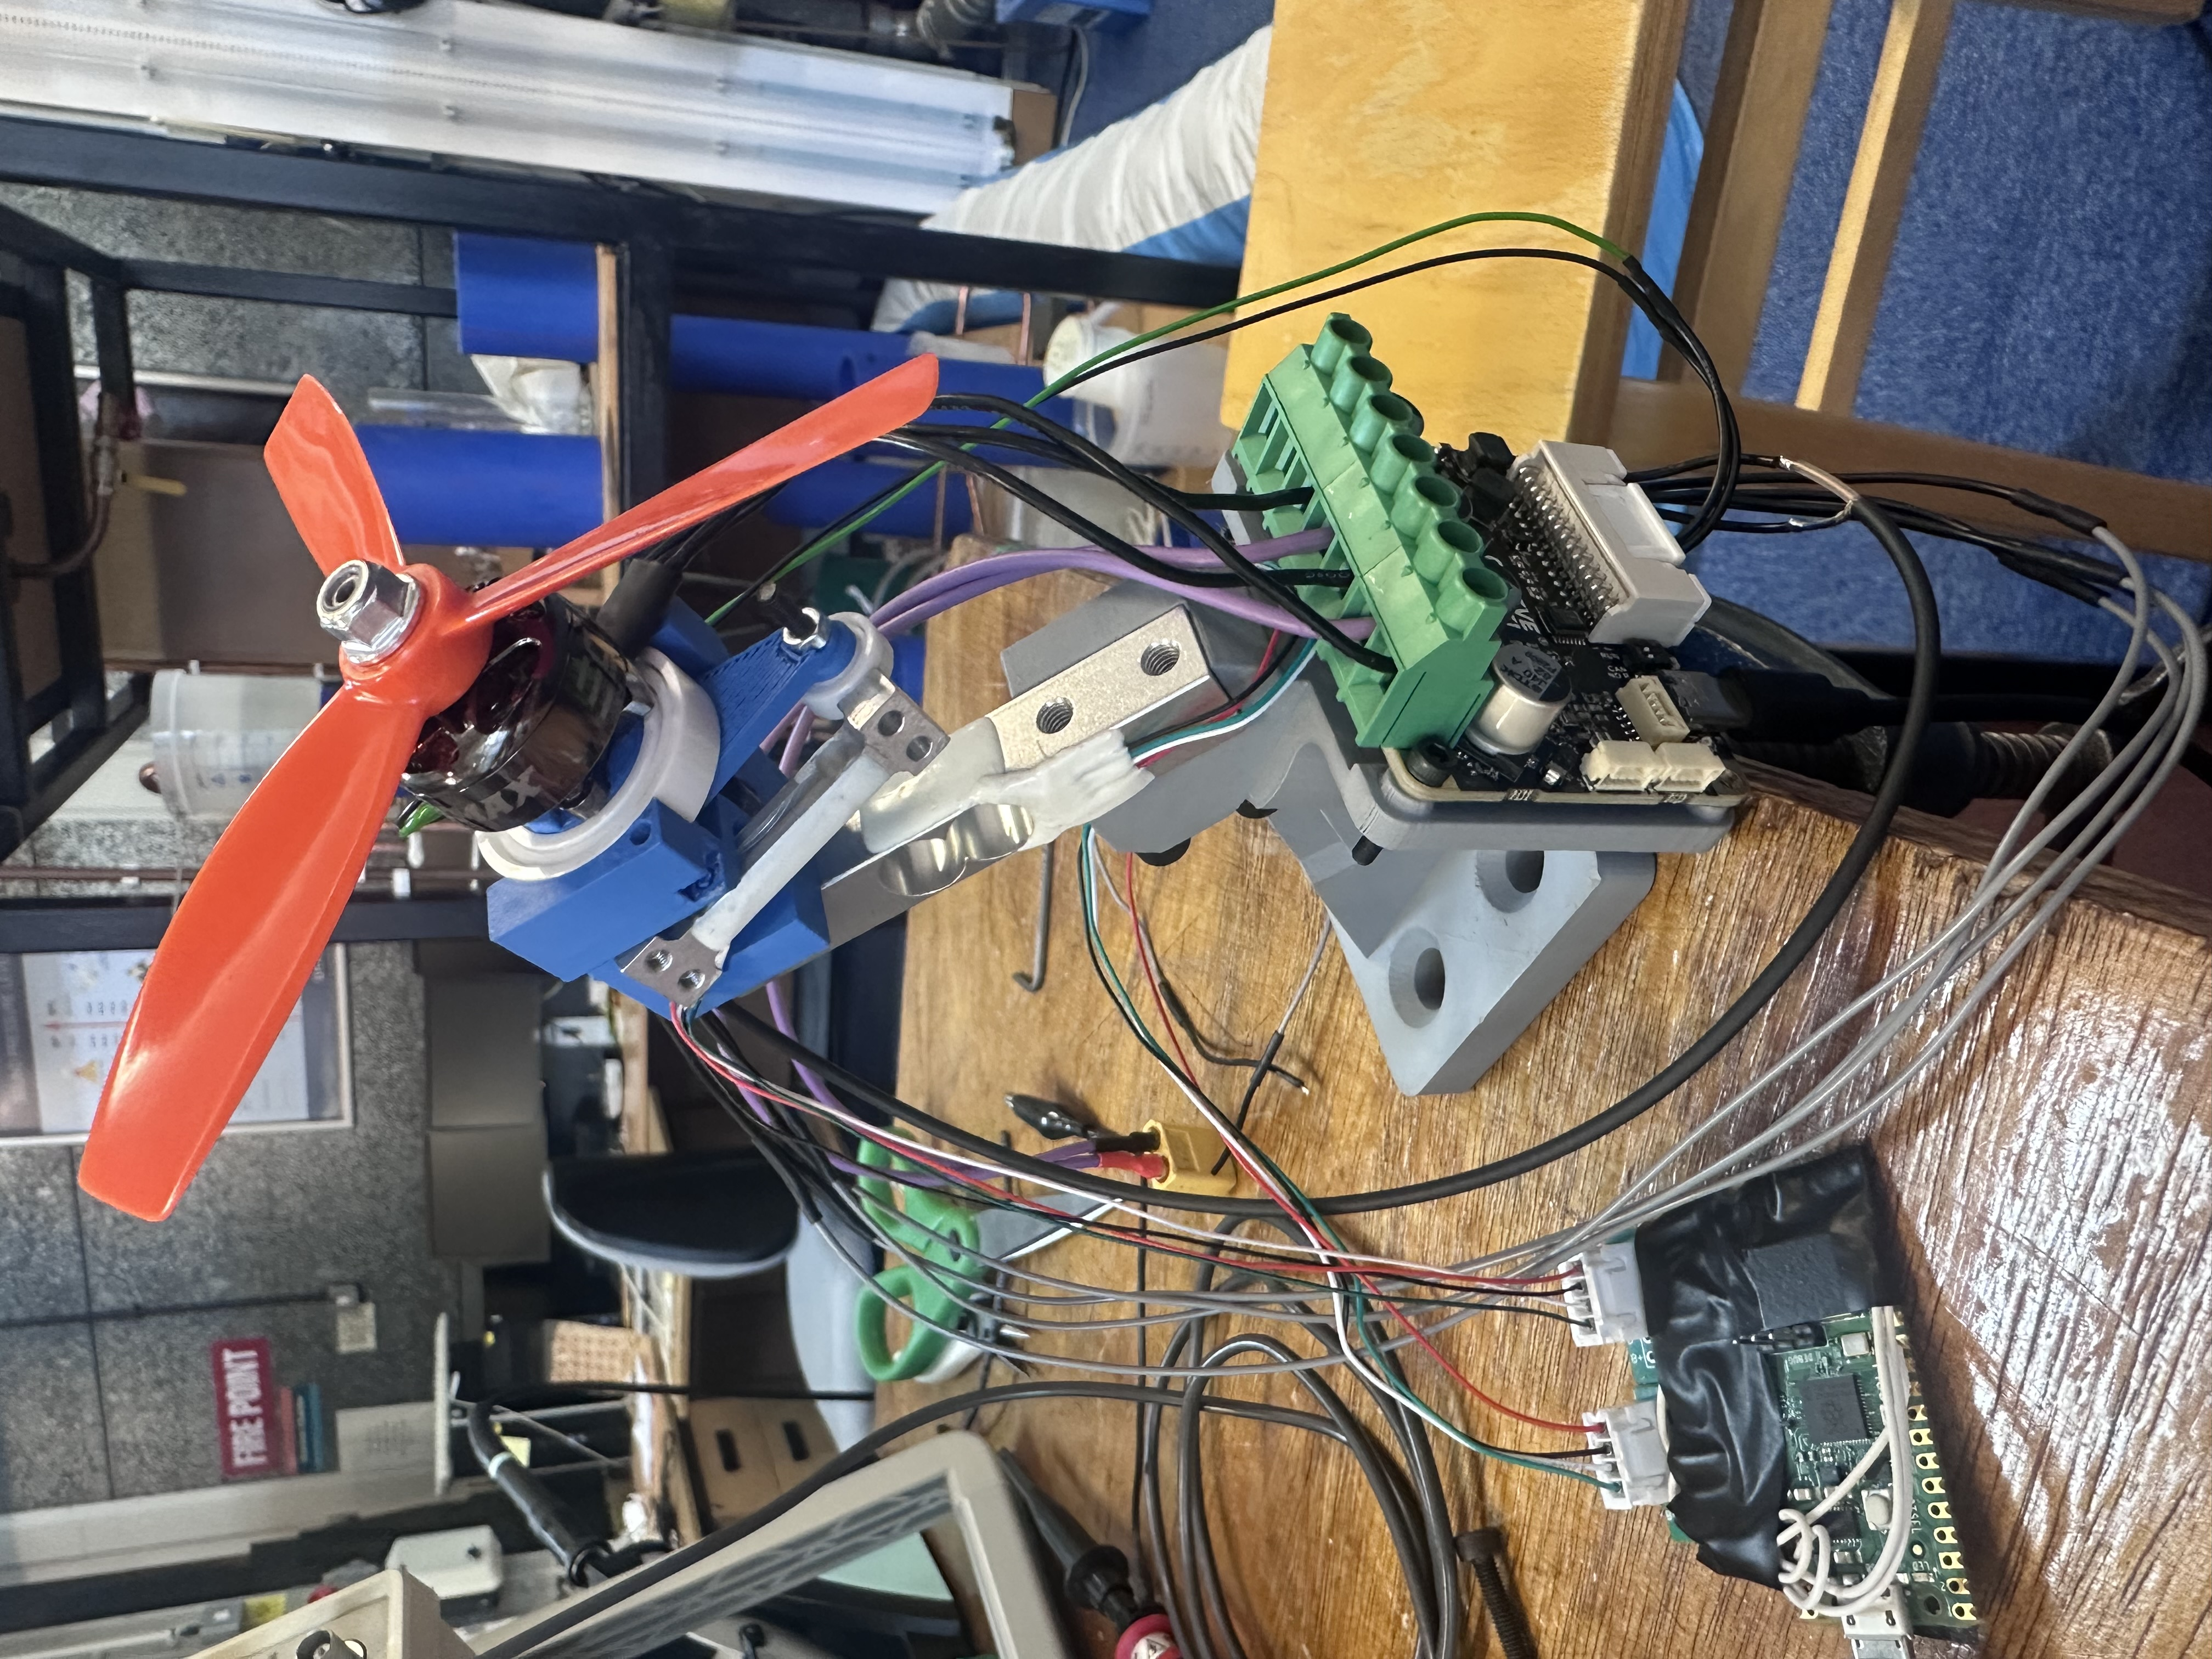
\includegraphics[height=8cm]{../figures/aero_setup.pdf}
            \caption{Assembled rig }
            \label{fig:assembled_aero}
        \end{subfigure}
        \caption{Aerodynamic test rig with moving platform and 200g load cell.}
\end{figure}

\begin{figure}[H]
   
\end{figure}
% show the setup used and explain the components

% 200g, 1Kg load cells, hx711@10Hz pi pico. Odrive S1, AS5047p encoder, 10kOhm motor thermistor
% explain some of the choices made in the setup
% explaination of calibration procedure
% extrapolation of thrust and torque coefficients
% control of variables 

\subsubsection{Acoustic setup}
% show the physical setup used and explain the components
% explain some of the choices made in the setup
% control of variables
The acoustic setup was concerned with measuring the far field harmonic sound of the propeller alone.
This was done in an anechoic chamber to prevent reflections from the walls.
An acoustic foam box was designed around the motor to isolate the motor noise from the propeller noise.
Structural vibrations from the motor on the rigid frame were damped by rubber feet.

From rubber feet geometry, typical material properties and the mass of the stand, the natural frequency of a second order system model was estimated to be 70.9 Hz \ref{sec:appendix_stand_frequency}.
This means that frequencies above this are attenuated by the stand and should not be present in the acoustic data.
Smaller speeds tested \~4000 RPM could excite this mode and produce noise in the acoustic data, however this was not observed in the sound spectrum.
% vibration
% motor pole count and frequencies
% acousic isolation inside the foam box
% acoustic isolation worsened vibration noise ?
A significant limitation was the maximum motor temperature of $80^\circ$ C.
This limited the maximum maintainable speed to 17000 RPM, for the short duration of 1s before having to ramp back down the speed.
A compressed air gun was used to cool the motor between tests.

% box vs no box
% floor test

\begin{figure}[H]
    \centering
    \begin{subfigure}{0.4\textwidth}
        \centering
        \includegraphics[height=8cm]{../tikz/mic_floor_plan.pdf}
        \caption{Floor plan}
        \label{fig:floor_plan}
    \end{subfigure}
    \begin{subfigure}{0.5\textwidth}
        \centering
        
\includegraphics[height=8cm]{../figures/chamber.pdf}
        \caption{Chamber view}
        \label{fig:anechoic_chamber}
    \end{subfigure}
    \caption{Acoustic test rig in the anechoic chamber.}
    \label{fig:test_rig}
\end{figure}

Seven GRAS 46BL microphones were sampled at a rate of 51.2 kHz from a National Instruments cDAQ9178.
Four microphones were mounted to stands at key angles $0^\circ$, $180^\circ$ and two at $90^\circ$ but at different azimuthal angles.
The remaining three were mounted on a movable gantry with two at a fixed distance either side from the central microphone.
For each propeller and distance, the gantry was moved between three equally spaced angular positions $[112.5^\circ, 135^\circ, 157.5^\circ]$.
A diagram showing the floor plan of the setup is shown in figure \ref{fig:floor_plan}.
At each position, an audio pyramid test was performed which, similar to the aerodynamic pyramid,
records audio at logarithmically increasing and decreasing speed values.
Propellers were swapped out between pyramid tests, then the gantry was moved to the next position.
When the gantry had visited all three positions, the microphones were moved to the next distance.
All propellers were tested at three distances 6, 8 and 10 blade diameters but the dalprop5045 was tested at more distances.
A piece of string was attached from the gantry to below the propeller to ensure the same distance was maintained at each gantry position.

The far field is where $R/r_t >> r_t \cdot mf_0 / c_0$.
For a propeller of radius 8cm spinning at 17000 RPM the far field approximation would start to break down for the first harmonic at
$ R/r_t \approx 0.4$. At the 10th harmonic this would be $R/r_t \approx 4$.
This means even the closest distance and highest speed the distance of 6 blade diameters will be in the far field for at least small harmonics.

% aero pyramid
% audio pyramid

% figure

% nidaqmx had to write to file to prevent data loss
% buffers were filled in each thread, and transferred to the main thread for plotting in the GUI.
% control saftey features were implemented such watchdog timers, speed and current limits.

\subsubsection{Data Processing}

% handling of audio data

Spectral leakage was minimised by applying a Hanning window to the audio data before the Fourier transform.
The window was normalised to have a root mean square (RMS) value of 1 to prevent the SPL from being affected by the window.
The audio data was calibrated by correcting the transformed signal by the interpolated factor at each frequency bin.

% rms normalised hanning window to prevent spectral leakage
% frequency domain interpolation of microphone calibration data

% method of integrating harmonics and definition pf HSPL
The harmonics had to be numerically integrated to obtain $OASPL_m$ from equation \ref{eq:OASPLm}.
Despite the Hanning window, spectral leakage still caused the broadening of the harmonic peaks.
The frequency bin width is $ \Delta = 51200 / 56000 = 0.914$ Hz, and numerical integration between the bounds $ m f_0 \pm 2 \Delta $ 
was found to capture the peak.
This corresponds to $\pm2$ frequency bins around the harmonic centre frequency $m f_0$.


\subsection{Propeller Design Tool}

A propeller design software tool was developed instead of using a standard parametric modelling software.
This allowed for fast iterative design, with the ability to quickly change propeller geometry and see results in real time.
A flowchart of the software is shown in figure \ref{fig:flowchart}.
First, a propeller must be sufficiently defined by editing the input table, or a \texttt{*.prop} file is loaded.
An airfoil profile is required which must be loaded from a \texttt{*.surf} file in the standard UIUC format \cite{uiuc_database}.
Standard air and operating conditions have default values, but can also be edited.

The software first runs a well known panel method solver, XFOIL, to compute the aerodynamic coefficients for the defined arbitrary airfoil.



\begin{figure}[H]
    \centering
    \includegraphics[width=0.8\textwidth]{../tikz/software.pdf}
    \caption{Flowchart of the propeller design software.}
    \label{fig:flowchart}
\end{figure}

% tradeoff between high lift to drag ratios because of trig functions

\begin{figure}[H]
    \centering
    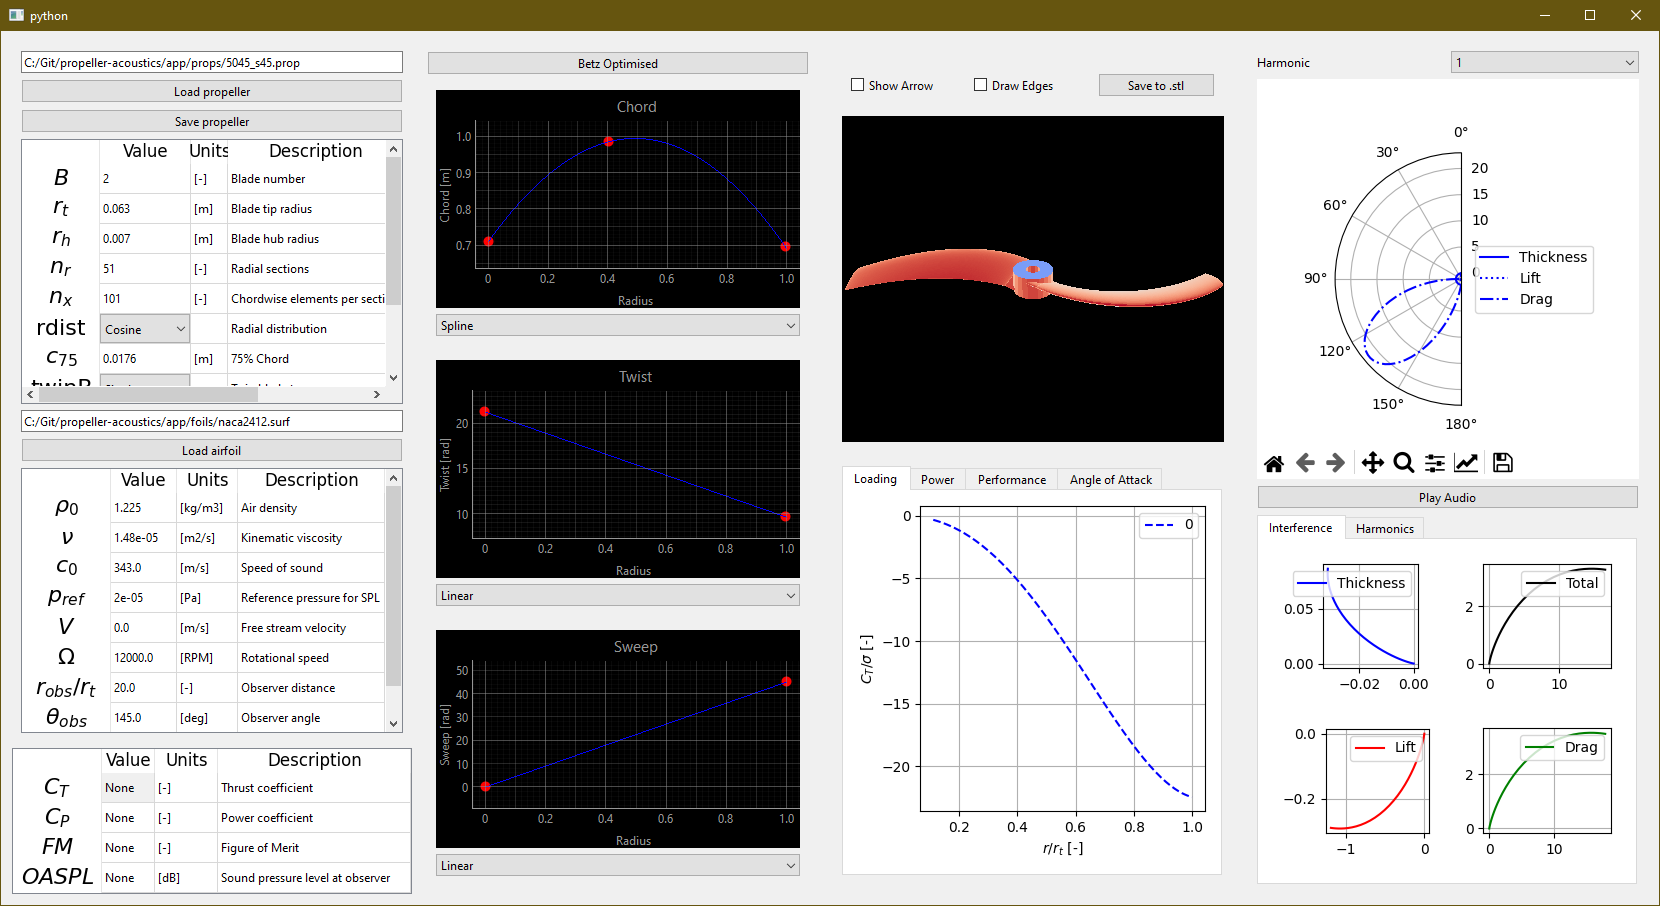
\includegraphics[width=0.8\textwidth]{../figures/design.pdf}
    \caption{Screenshot of the propeller design software.}
    \label{fig:design_software}
\end{figure}

% explain how 3d files are generated
The software generates an STL file of a propeller by merging $B$ single blade meshes with a hub mesh.
The blade mesh is generated by defining a series of airfoil coordinates along the span of the blade, scaled by the local chord.
The airfoils are then rotated around the span axis by the local twist, and then the airfoil plane is rotated around the hub axis by the local sweep.
Triangles are then generated, two for each airfoil point to fill the squares between adjacent airfoil points.
Code by Lily Board \cite{board2025blade} was used to generate the triangles.

The looped propeller designs were generated by continuing from its original tip, along a hermite curve, back to the same axi-symmetric blade with reversed sweep.
A hermite curve is a polynomial curve defined by two points and two tangents.
The points are known from the original and new tip of reversed sweep blade.
The tangents found at both tips from the gradient of sweep angle.
However, when the airfoil is swept around, it must be flipped to ensure the leading edge is always facing the direction of rotation.
This causes the triangle generation to be more complicated at the tip to avoid being twisted.


% available propeller design tool input
% python implementation of the nonlinear solver and acoustic model
% airfoil coefficient interpolation and extrapolation
% explain the propeller mesh generation algorithm and minimum airfoil thickness


\subsection{Propeller Designs}
% explain choice of simple linear swept blade designs

Five commercial off the shelf propeller designs were bought for the project, four Dalprop designs shown in figure \ref{fig:dalprop_series} and one Foxeer looped design shown in figure \ref{fig:loop_series}.
This was to compare the performance of 3D printed propellers to standard propellers used in the industry.
The dalprops from left to right are 5045bnr, 4045, 5045, 6045.
The convention is that the first two digits represent the diameter in inches and the last two digits represent the pitch.
This means that 5045 has a diameter of 5 inches and a pitch of 4.5 inches.
The simple twist distribution is found from local radius $r$ and pitch $p$ of the propeller.
\begin{equation}
    \beta = \alpha + \arctan \left( \frac{p}{2\pi r} \right) \label{eq:twist}
\end{equation}
Where the angle $\alpha$ is an optimum angle of attack for the airfoil.
Ten propellers were manufactured from the models generated by the software.
Clones of the 5045bnr and 5045 were printed, shown in figure \ref{fig:sweep_series}, along with a series of swept propellers.
The sweep distributions were chosen to be linear up to 15, 30, 45 and 60 degrees at the tip.
The 3D printed designs had slightly thicker ClarkY airfoil sections to account for the weaker 3D printed material, and additional torsion from sweep.
The propellers were otherwise identical to the printed 5045 for consistency.
% do i explain that i couldnt get an optimised propeller printed because of bet solver failure?
The propellers were printed on an Objet30 3D printer using a photopolymer resin.
The design software was modified to set a minimum airfoil thickness of $2\times28$ microns,
corresponding to twice the minimum layer height of the printer to ensure a smooth trailing edge.

\begin{figure}[H]
    \centering
    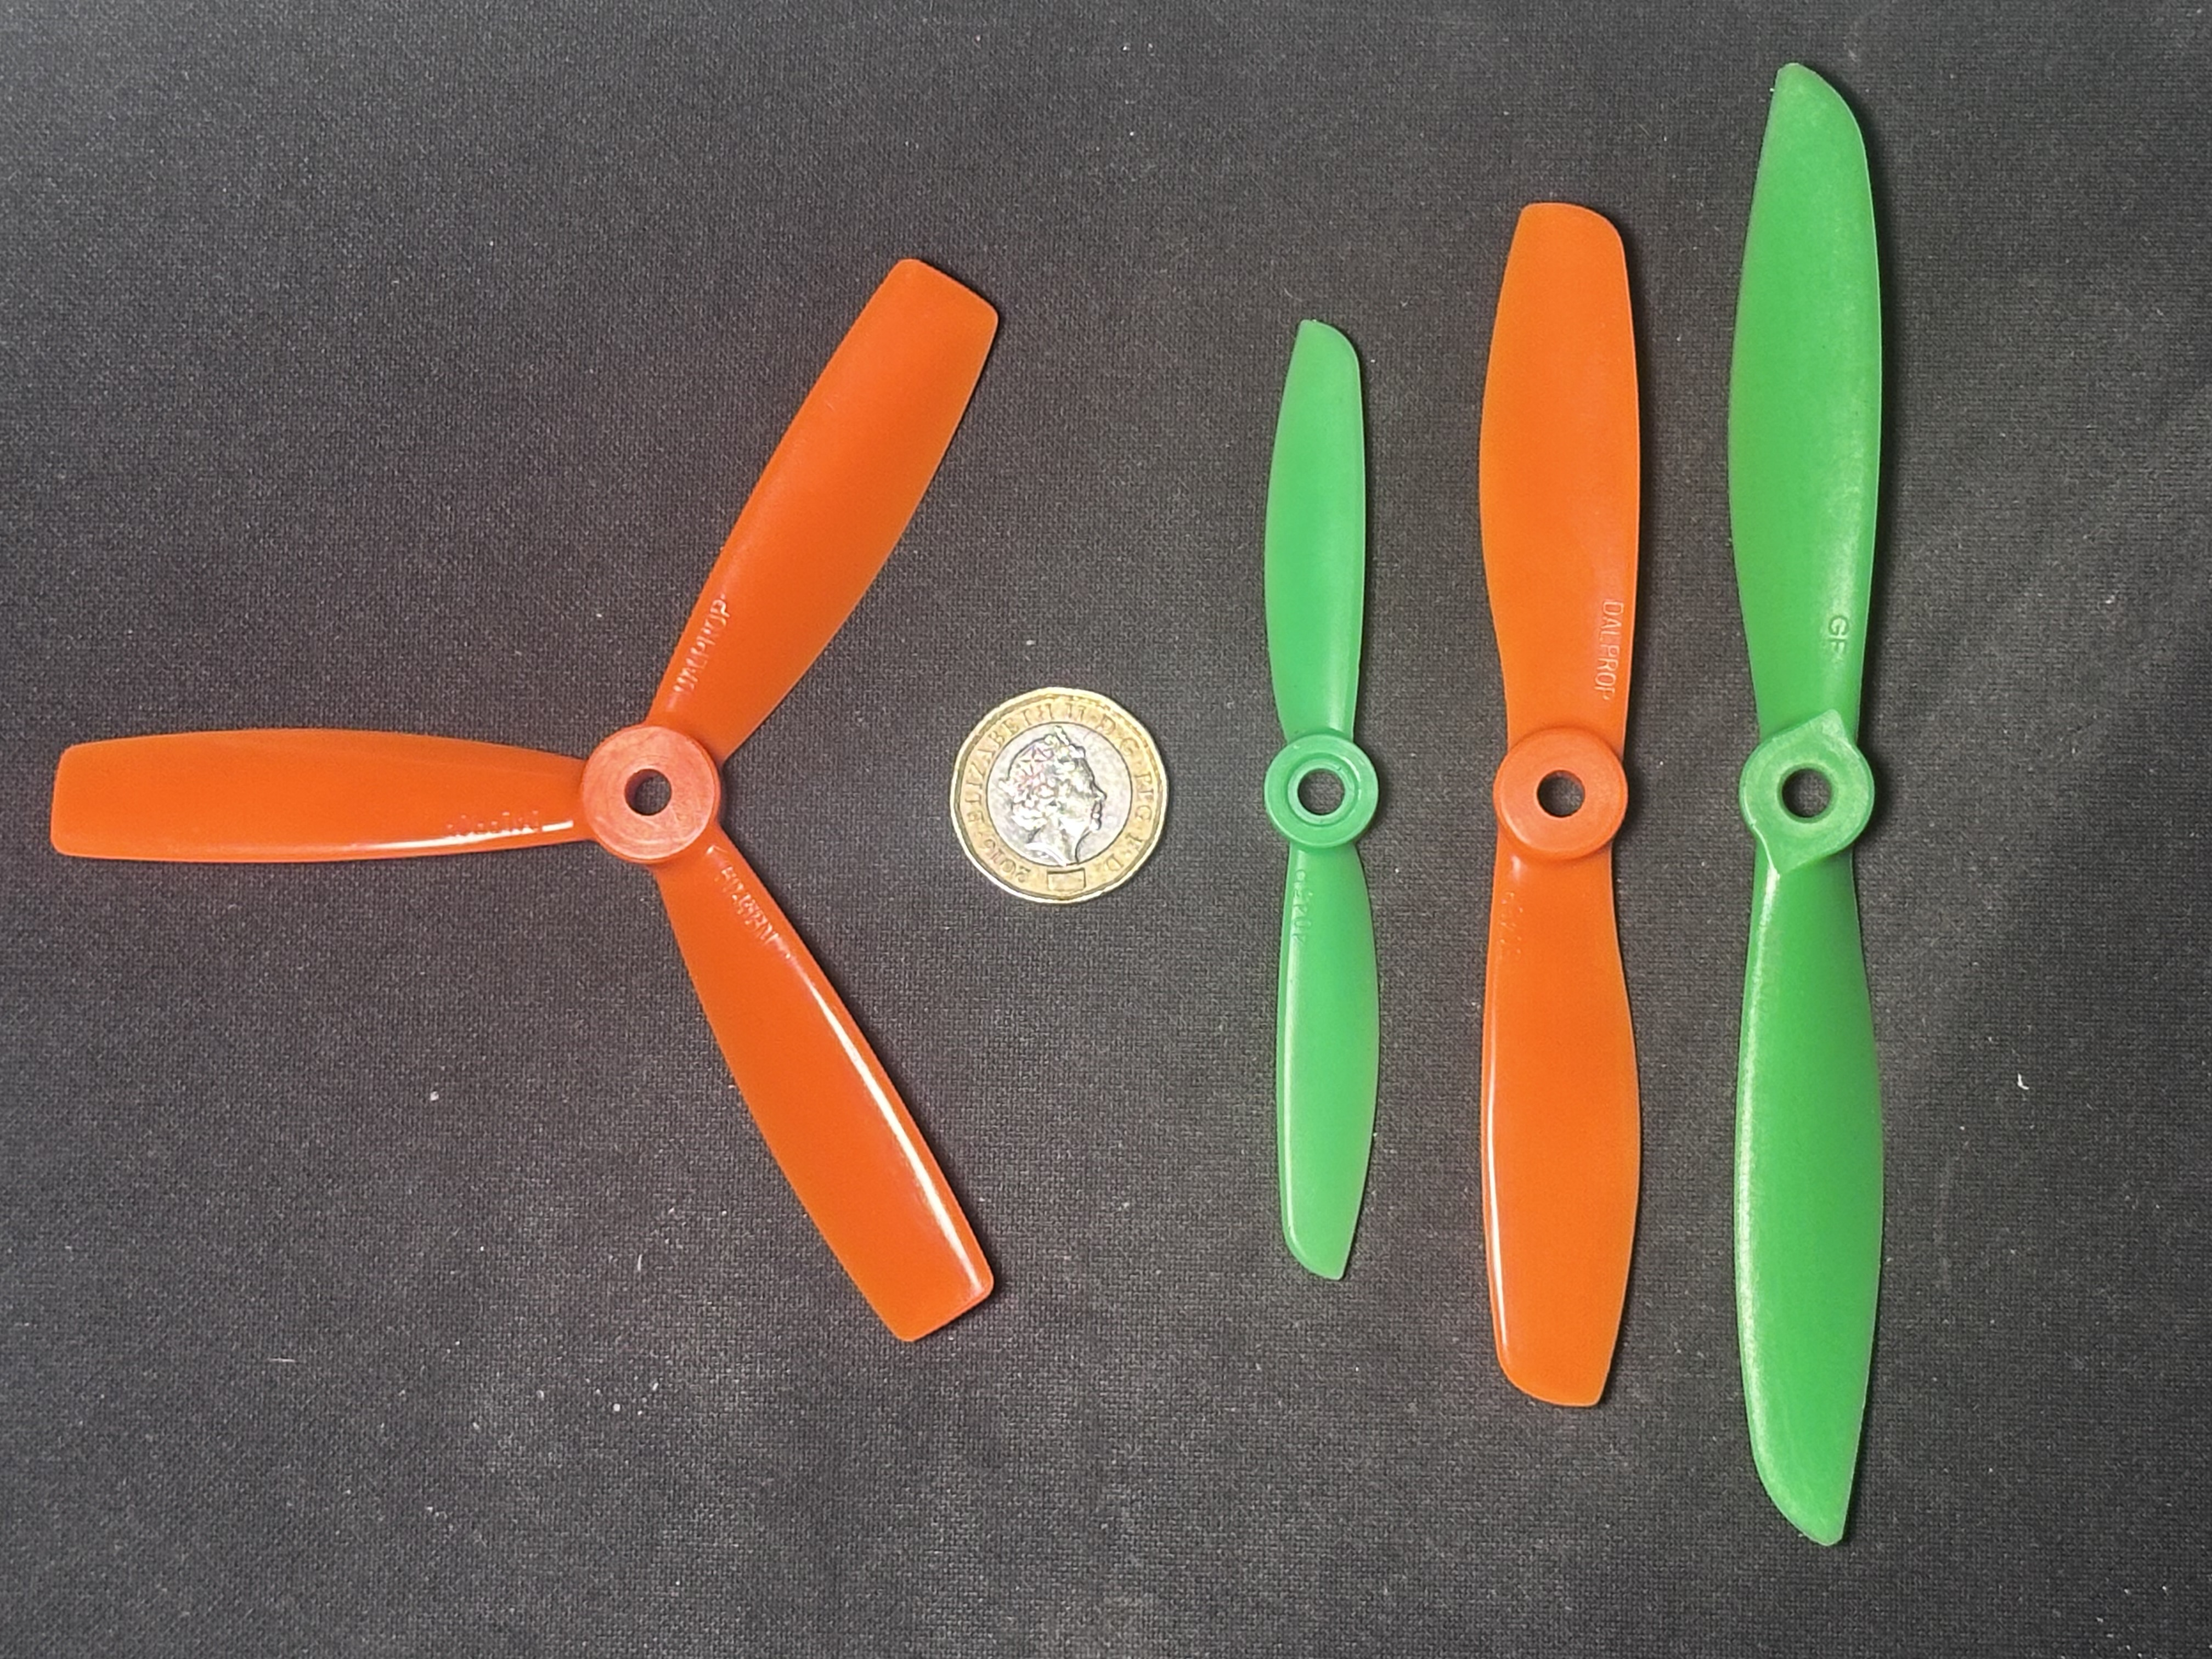
\includegraphics[width=0.8\textwidth]{../figures/dalprop_series.pdf}
    \caption{Commercial dalprop propeller designs. From left to right: 5045bnr, 4045, 5045, 6045.}
    \label{fig:dalprop_series}
\end{figure}

\begin{figure}[H]
    \centering
    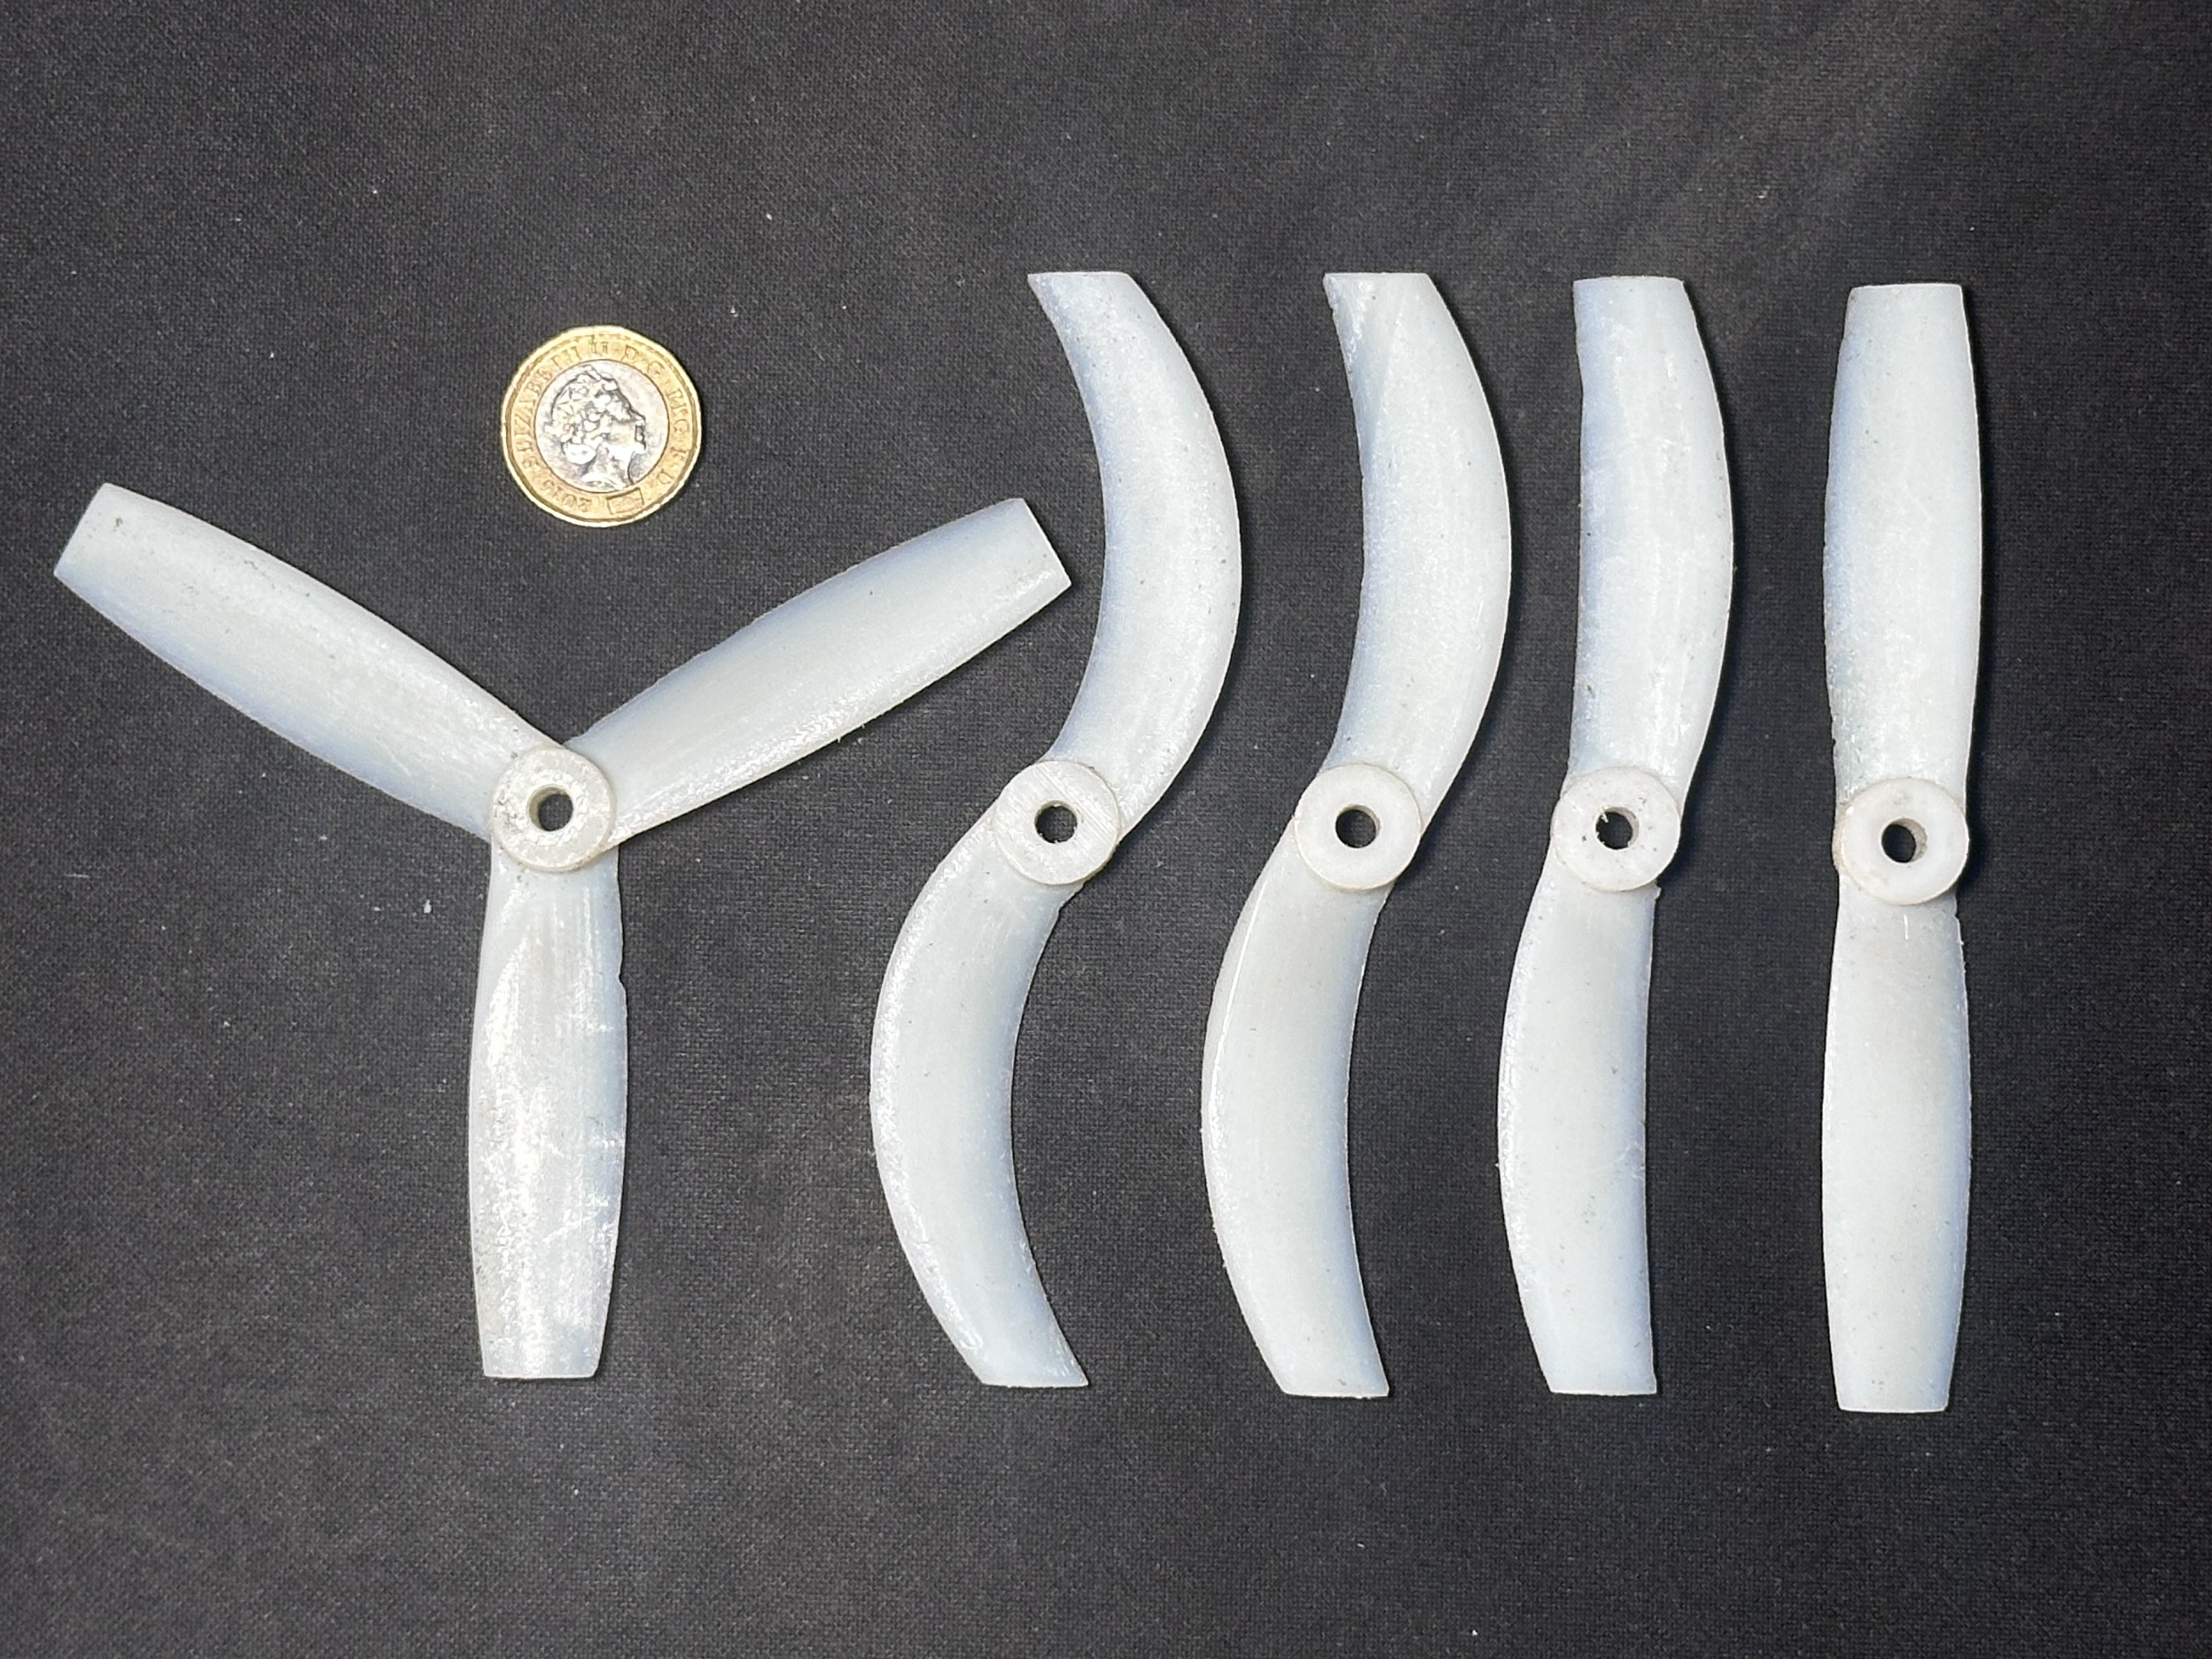
\includegraphics[width=0.8\textwidth]{../figures/sweep_series.pdf}
    \caption{Swept propeller designs used in the project. From left to right: printed5045bnr, 5045\_s45, 5045\_s30, 5045\_s15, printed5045}
    \label{fig:sweep_series}
\end{figure}

\begin{figure}[H]
    \centering
    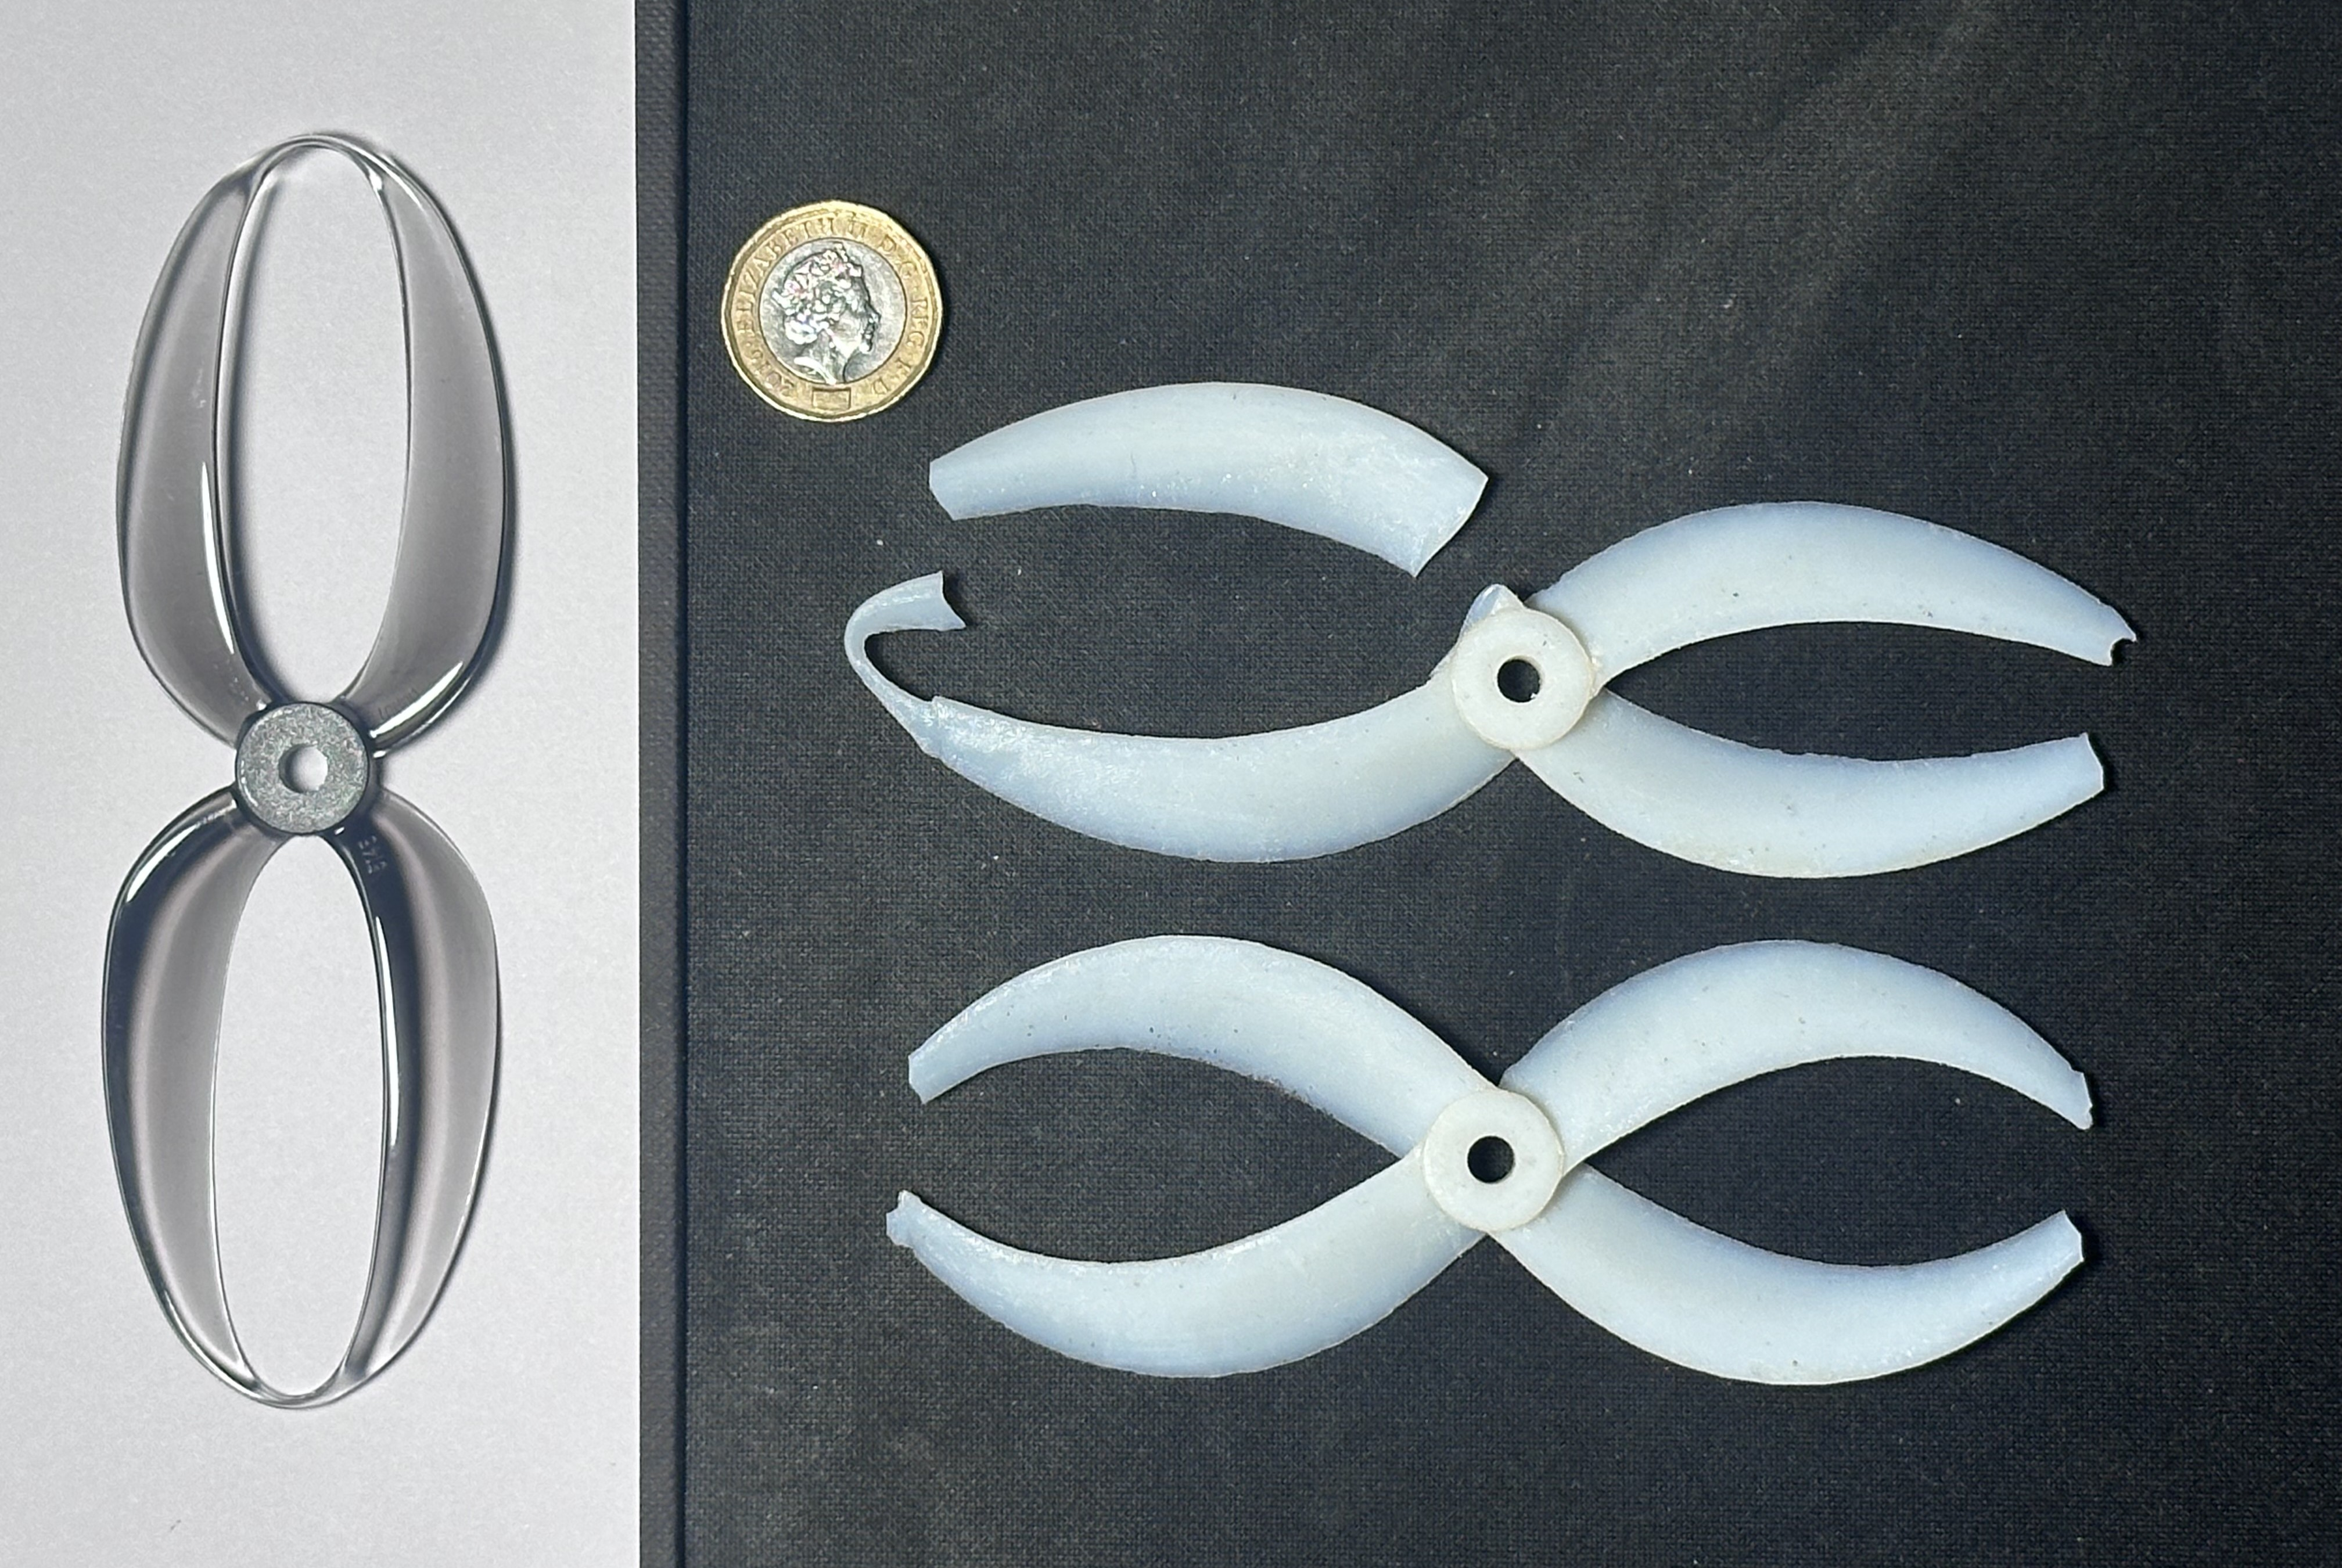
\includegraphics[width=0.8\textwidth]{../figures/loop_series.pdf}
    \caption{Looped propeller designs. Commercial foxeer\_toroidal on the left, printed 50loop\_s40 on top and 50loop\_s50 below.}
    \label{fig:loop_series}
\end{figure}

From the images taken after testing, it can be seen that both looped designs were damaged during testing.
The 50loop\_s40 suffered a break at the hub and tips, whereas the 50loop\_s50 suffered a break at the tip.
A highly swept $60^\circ$ propeller was also designed and printed, but broke at the mid-span during testing.

These breakages highlight the different material strengths, with the tip for the Foxeer propeller being thinner than that which broke on the printed propeller.
After the 50loop\_s40 broke, the 50loop\_s50 was spun up to a reduced speed of 13000 RPM, but broke at its tips after a few test runs.
This indicates, from the cyclic loading of accelerating and decelerating, that the tips met their fatigue limit.

\section{Results and Discussion}

% paragraph for every graph explaining every feature
% explain theoretical results and how they compare to experimental results

% discuss in great detail errors sources and uncertainties
% differences between aero and acoustic setups?
% poor load cell calibration
% microphone interference sources
% microphone position uncertainty (very large)

\subsection{Calibration}

\begin{figure}[H]
    \centering
    \includegraphics[width=0.99\textwidth]{../tikz/loadcell_caltab.pdf}
    \caption{Calibration graphs for the load cells used in the aerodynamic setup.}
    \label{fig:loadcell_caltab}
\end{figure}

Figure \ref{fig:loadcell_caltab} shows the applied forces and measured signals during separate calibration tests.
As expected, the thrust load cell has a strong linear relationship between the applied force and the measured signal.
Similarly, the applied torque is strongly linear with the measured signal in the range of calibration.
The applied torque influences the reading on the thrust sensor, which shows a weakly linear relationship.
This is likely due to not applying the torque in the plane load cell, due to tolerances and table flatness.
The key result is that the variation in thrust signal is 2 orders of magnitude smaller than the applied thrust signal.
%The variation of the torque signal due to applied thrust is shown to lie entirely within the error bars and is attributed to noise.
The variation of the torque signal due to applied thrust is shown to be small, such that the sensor noise error bars are visible.
However, there is still variation outside of these error bars, indicating out of plane forces and nonlinearities.
% This must be due to part of the thrust force being carried through the torque load cell rather than the ceramic bearing.
% This is friction and bearing tolerances, but this was not observed.

The torque due to the propeller is calculated from subtracting the no load torque from the measured propeller.
However, the no load torque at all speeds were measured to be negligible on the calibration curves.
This is likely due to smaller forces required to overcome friction of motor bearings compared to ceramic platform bearings.

The motors phase currents are measured by the controller and are used to calculate a torque producing current, $I$.
A torque constant $k_Q$, covered in more detail in the appendix \ref{sec:appendix_motor_calibration}, can then be used to calculate torque.

\begin{equation}
    Q = k_Q (I_\text{load}  - I_\text{noload}) \label{eq:torque_from_current}
\end{equation}

The equation is expected to be accurate for small motor currents and temperatures where load and noload losses are similar.
The presence of a control system, increasing the current to maintain speed when there are increased losses, further complicates the relationship.

\begin{figure}[H]
    \centering
    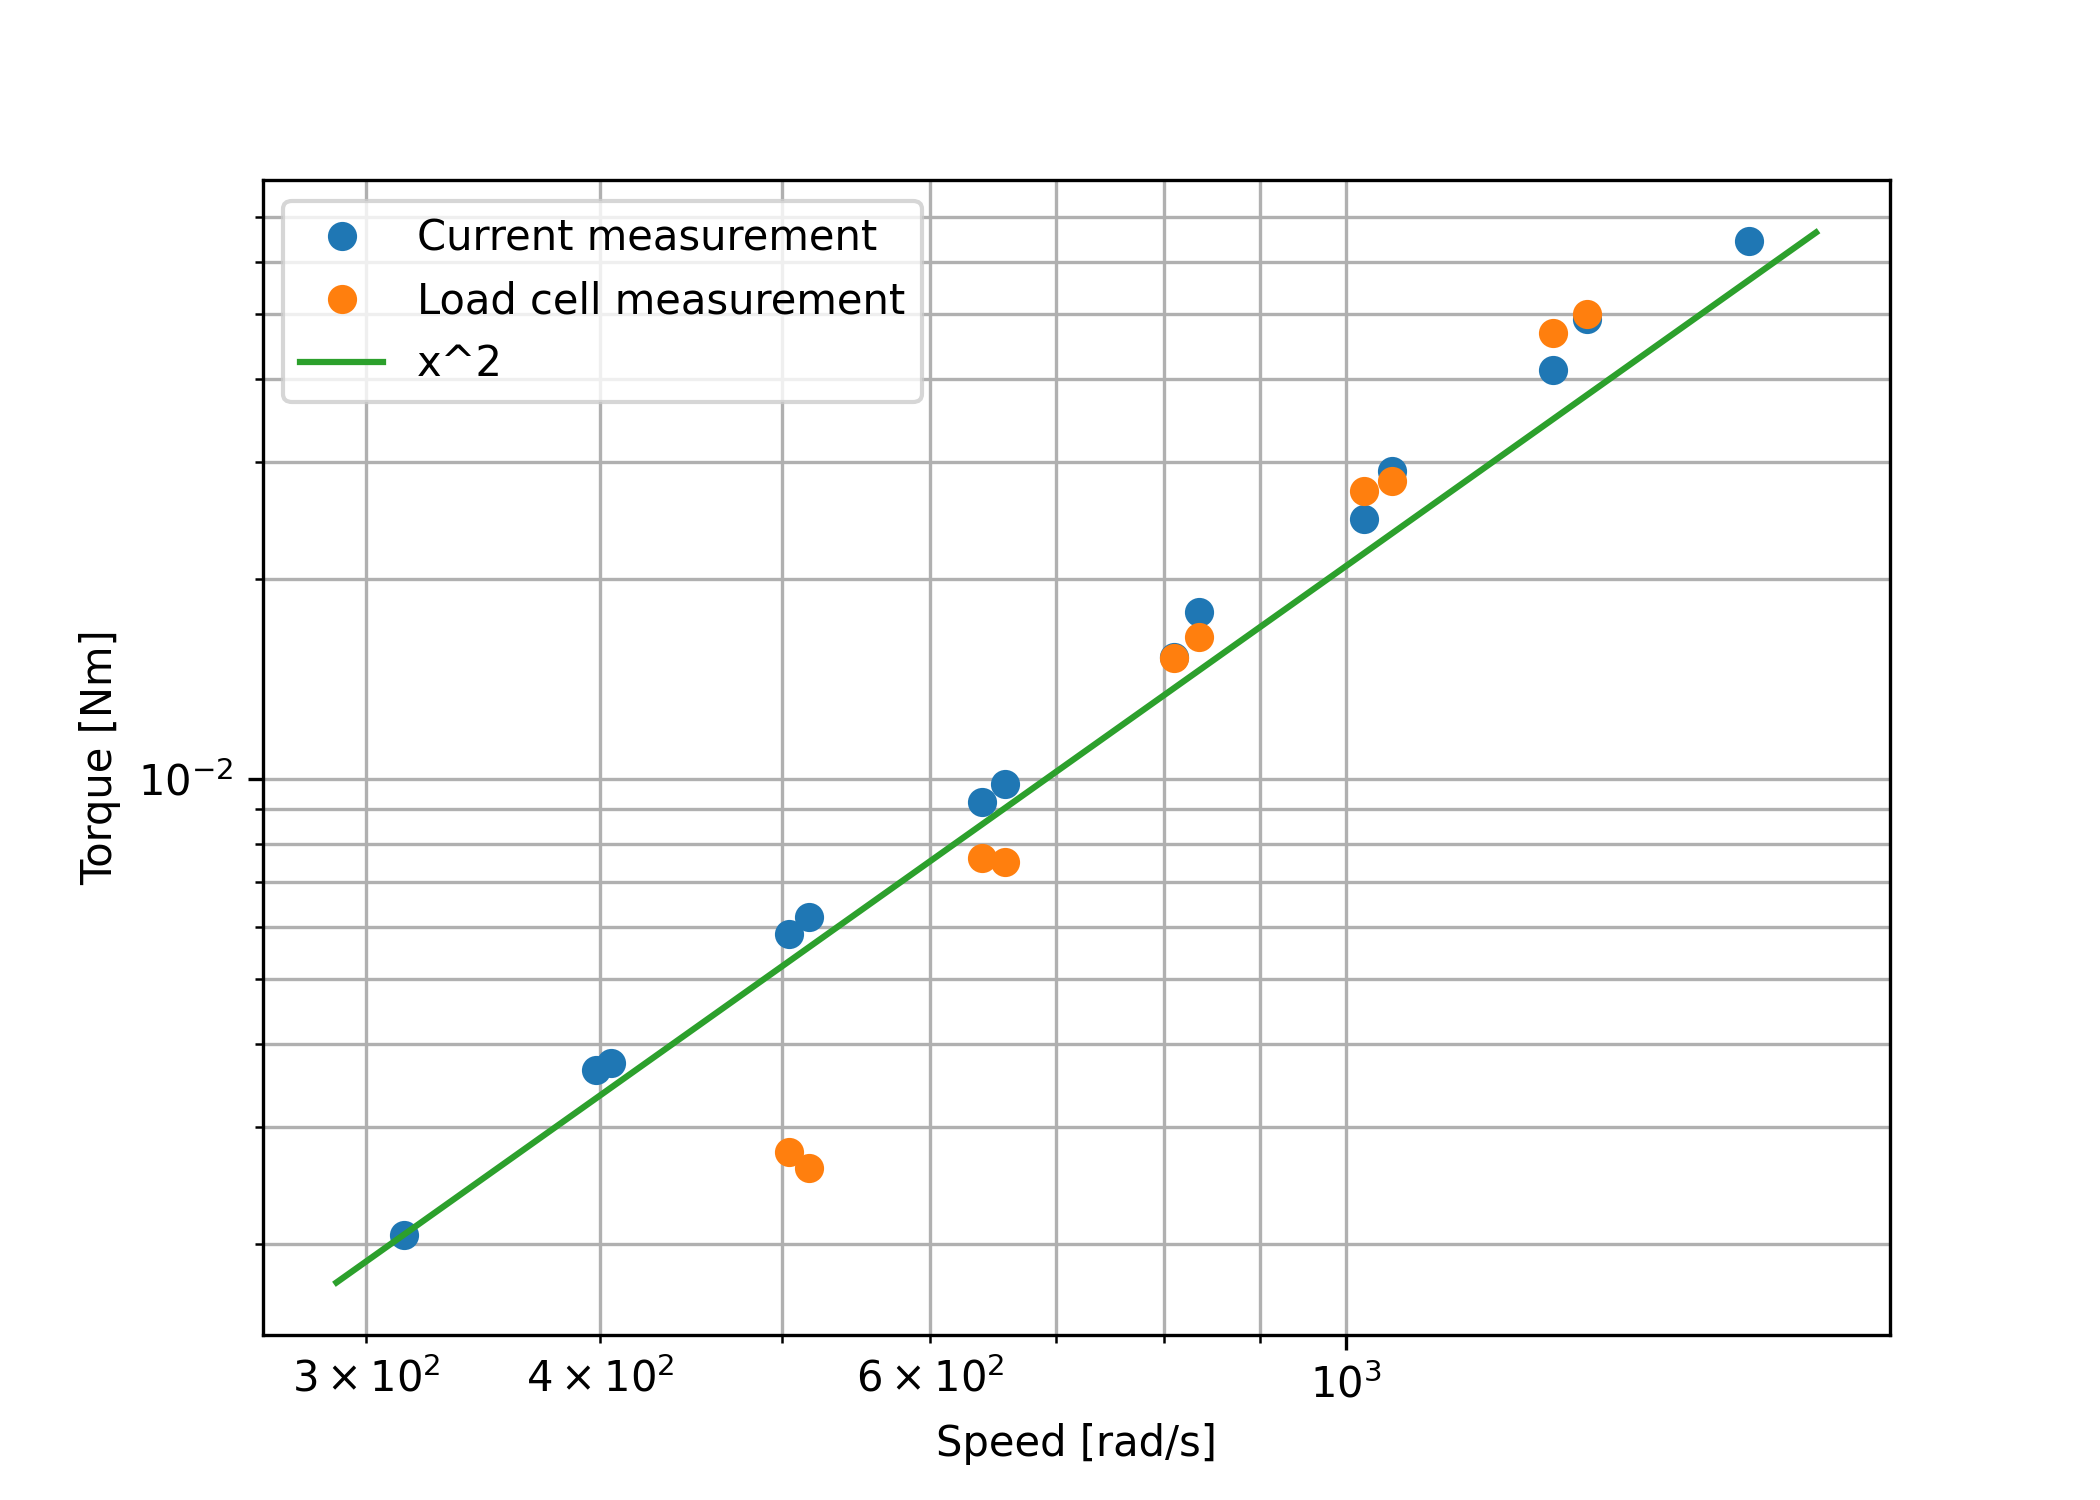
\includegraphics[width=0.8\textwidth]{../figures/controller_vs_loadcell_torque.pdf}
    \caption{Torque measured by calibrated load cell compared to torque calculated from measured motor current for the dalprop 5045bnr propeller.}
    \label{fig:controller_vs_loadcell_torque}
\end{figure}

Figure \ref{fig:controller_vs_loadcell_torque} shows the torque power law with speed.
Two points at each speed are shown which represents the measurements both on the way up and down the speed pyramid.
The load cell measurements are below the expected square power law for small values, likely due to similar friction in the bearings.
For high values of torque, the measurements agree with the power law.
The current calculated torque shows a strong agreement with the power law over the full range of speeds.
These values also agree within 7\% of the calibrated load cell values
This could be used at low torque values which were unable to be read by the load cell.


\begin{figure}[H]
    \centering
    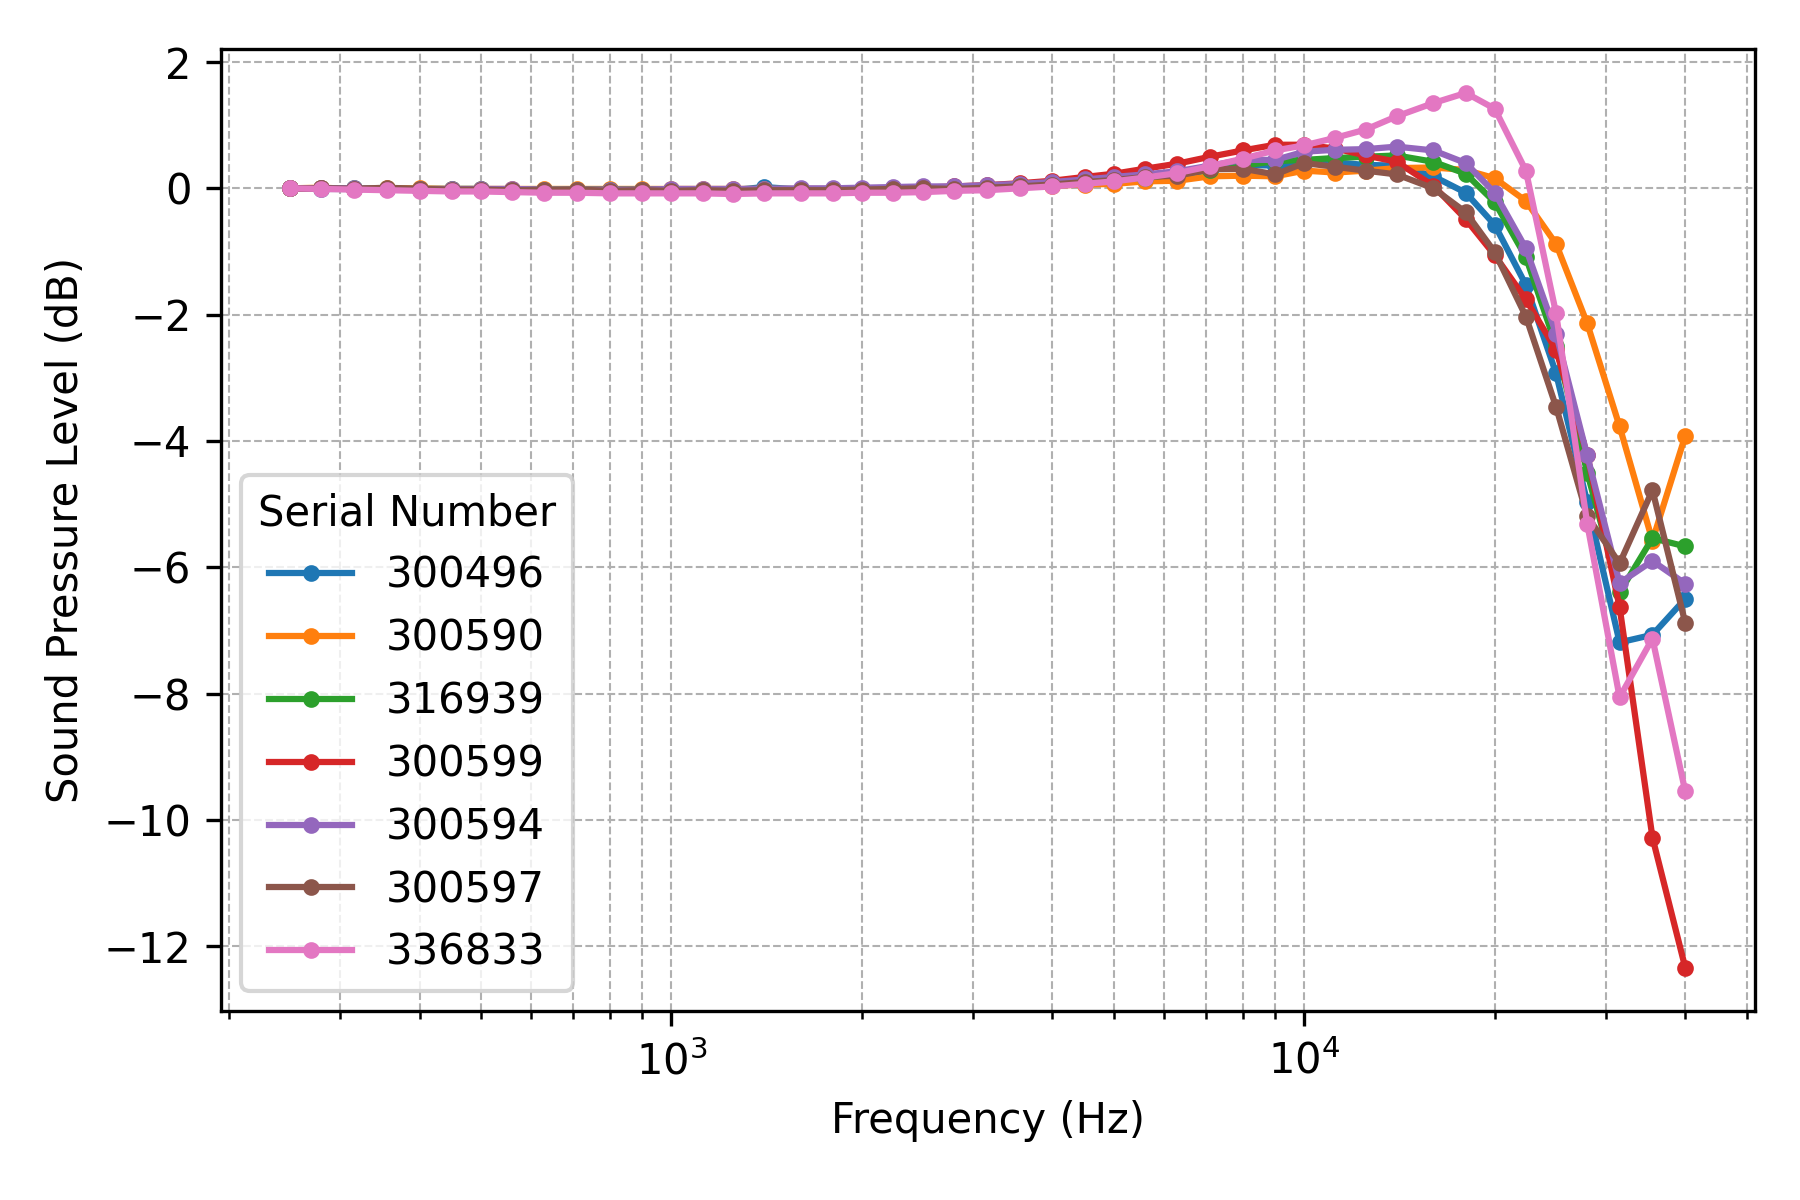
\includegraphics[width=0.8\textwidth]{../figures/microphone_calibration.pdf}
    \caption{Calibration graphs of the microphone used in the acoustic setup.}
    \label{fig:microphone_calibration}
\end{figure}

Figure \ref{fig:microphone_calibration} shows the calibration for the GRAS 46BL microphones used in the acoustic setup.
Low frequencies are shown to have little correction, while frequencies above the human range of hearing require correction.
GRAS guarantees the calibrated response to be within 2 dB up to 20 kHz.

\subsection{Aerodynamic performance}

\begin{figure}[H]
    \centering
    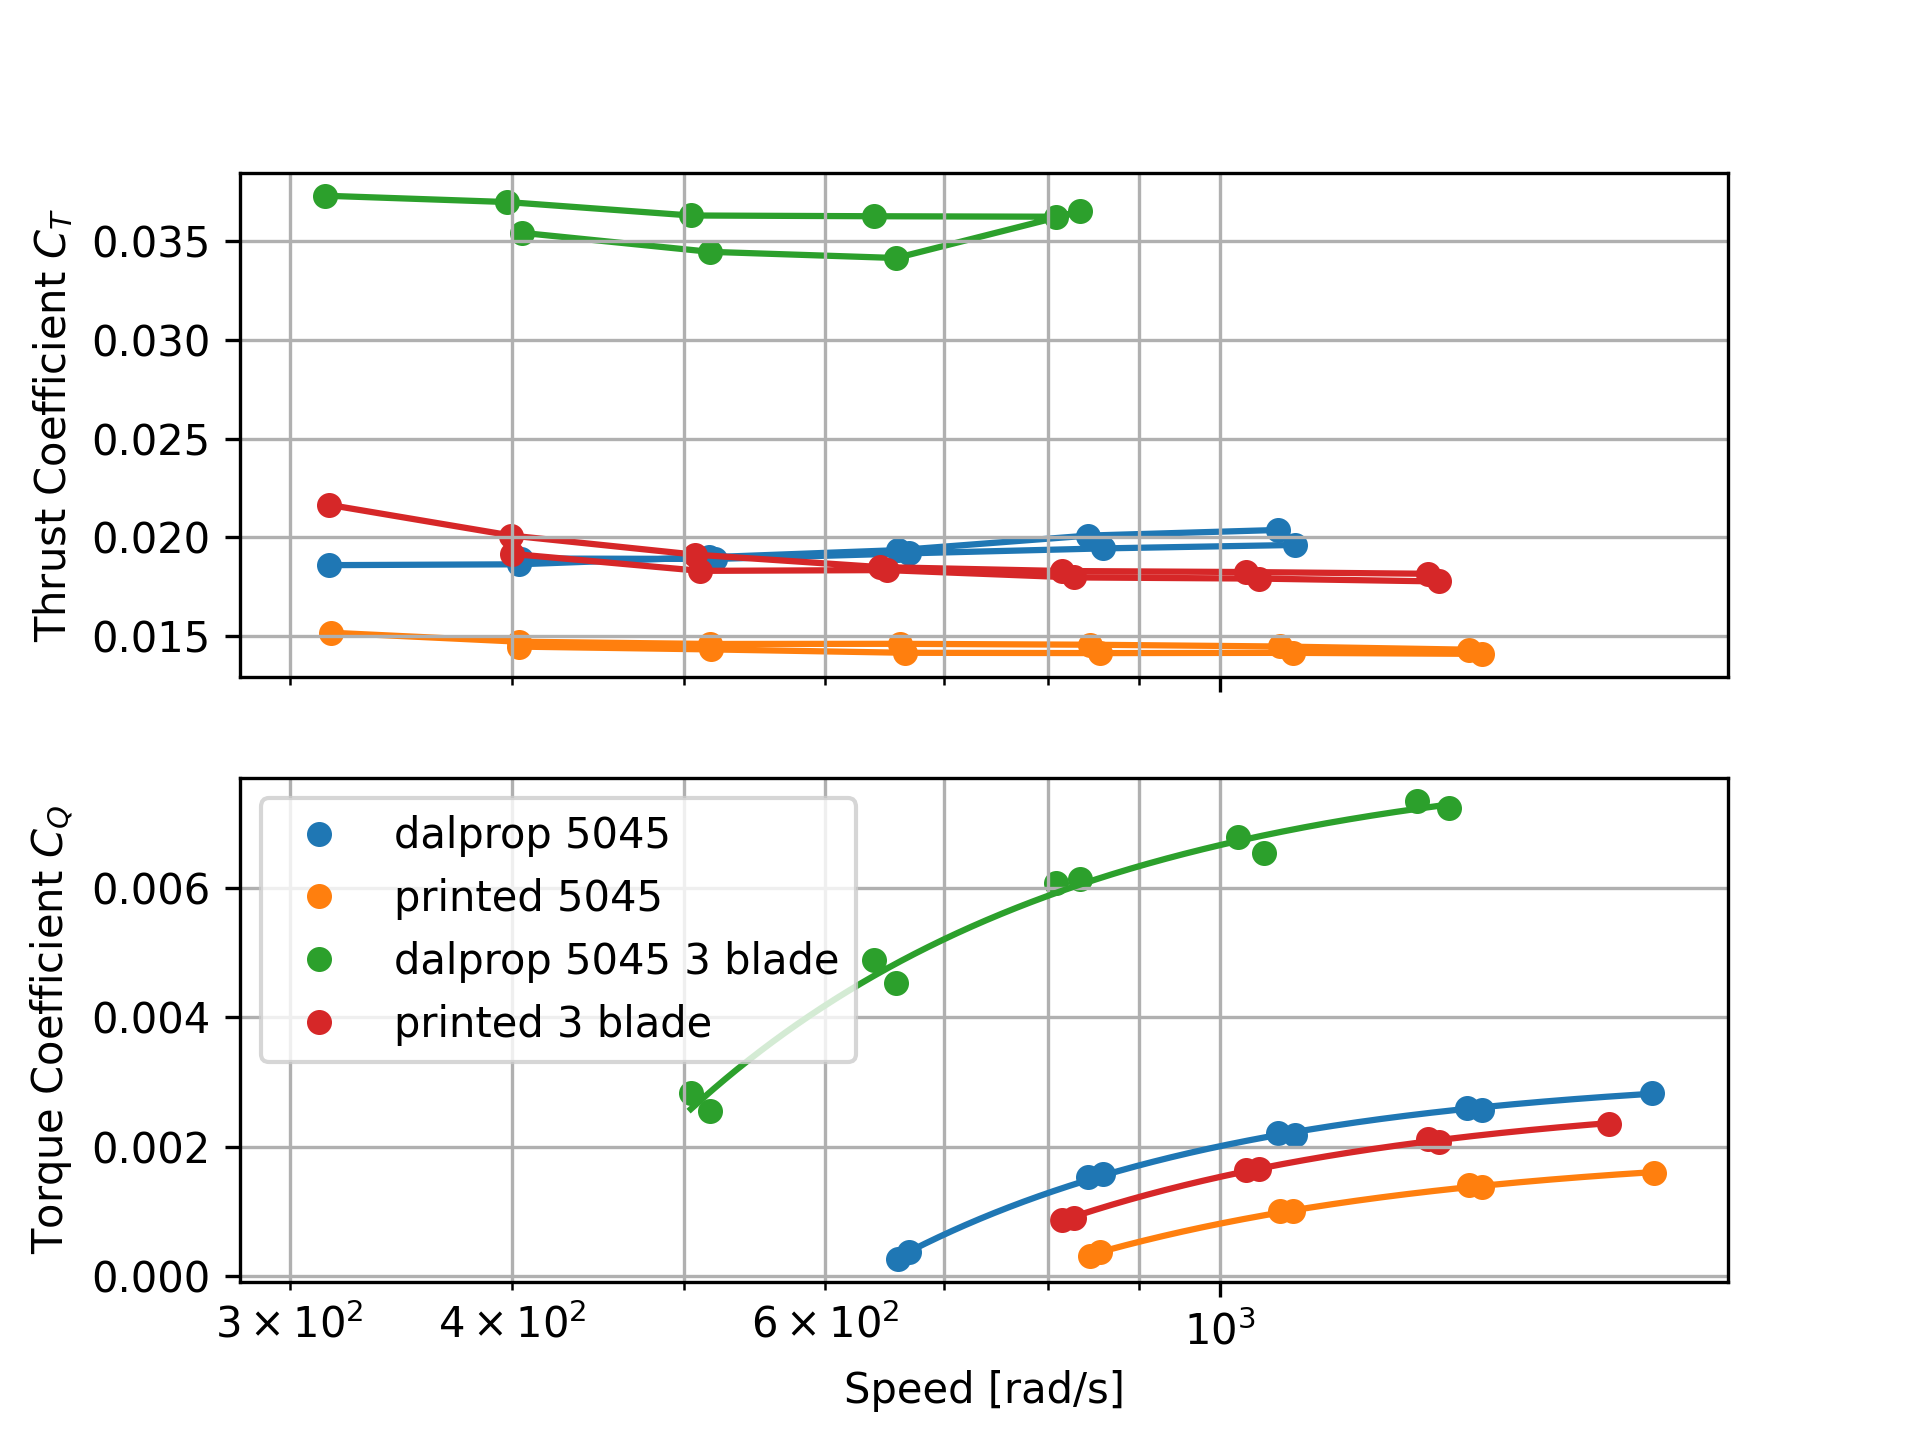
\includegraphics[width=0.8\textwidth]{../figures/printed_aero_coeffs.pdf}
    \caption{Thrust and torque coefficients for the printed propellers}
    \label{fig:printed_aero_coeffs}
\end{figure}

Figure \ref{fig:printed_aero_coeffs} shows the aerodynamic coefficients against speed for both the commercial propellers, and similar printed propellers.
It can be seen the thrust coefficients remain relatively constant over the range of speeds.
However, the torque coefficients show to increase with speed.
At higher values of torque, the speed dependence decreases shown by the flattening of the curve.
This agrees with previously discussed small bearing friction needed to be overcome by the torque platform.
This acts as a systematic error in the torque measurements, and so becomes less significant at higher measurements.
The small high speed bearings within the motor would likely have some speed dependence but this was ignored.
An asymptote curve was fitted to the measured coefficients to extrapolate when the error becomes negligible.
This was done for all tested propellers, with coefficients and figure of merits shown in figures \ref{fig:prop_aero_coeffs} and \ref{fig:prop_fms}.
This was not possible however, for the 4045, which only produced two data points within the range of speeds available to the experimental setup.


\begin{figure}[H]
    \centering
    \includegraphics[width=0.8\textwidth]{../figures/CT_CQ_bar.pdf}
    \caption{Thrust and torque coefficients for propellers}
    \label{fig:prop_aero_coeffs}
\end{figure}

Figure \ref{fig:prop_aero_coeffs} shows the thrust and torque coefficients for all propellers tested.
Error bars shown are propagated only from the standard deviation of speed and force measurements.
Uncertainty from the calibration is not included, but is expected to be small for thrust.
Torque has a larger component because of the small distance of 3 cm.
The error due to fitting the asymptote on torque is also not included but is expected to be large.

The thrust coefficient for dalprop5045bnr is 86\% higher than the similar dalprop5045.
Intuitively, a 50\% in coefficients would be expected from the additional blade.
This could be explained by reduced tip losses from the additional blade \cite{prandtl_loss}.
Comparing 3D printed versions of the dalprop designs show a reduction of 25\% and 48\% in thrust coefficient for 2 and 3 bladed models respectively.


\begin{figure}[H]
    \centering
    \includegraphics[width=0.8\textwidth]{../figures/FM_bar.pdf}
    \caption{Figure of merit of propellers}
    \label{fig:prop_fms}
\end{figure}

Figure \ref{fig:prop_fms} shows the figure of merit for all propellers tested.
The error bars are propagated from the errors in thrust and torque coefficient shown in figure \ref{fig:prop_aero_coeffs}.

The 5045\_s45 propeller is shown to have the highest figure of merit at 0.83.
The value is significantly higher than the similar geometry 5045\_s30, which shows a reduction from the 5045\_s15.
This reduction is thought to be due to reduced lift and drag coefficients acting at higher sweep angles.
The high FM of 5045\_s45 is then thought to be an error in the measurement of the torque for this propeller.
This can easily originate from the curve fitting of the asymptote to the torque coefficients.

The reference values for the thrust and torque coefficients were chosen to be the average coefficients accross all propellers tested.
This gives $K_T = 0.01535$ and $K_Q = 0.002812$ for a reference figure of merit of $FM_\text{ref} = 0.4781$.

\subsection{Acoustic performance}

\begin{figure}[H]
    \centering
    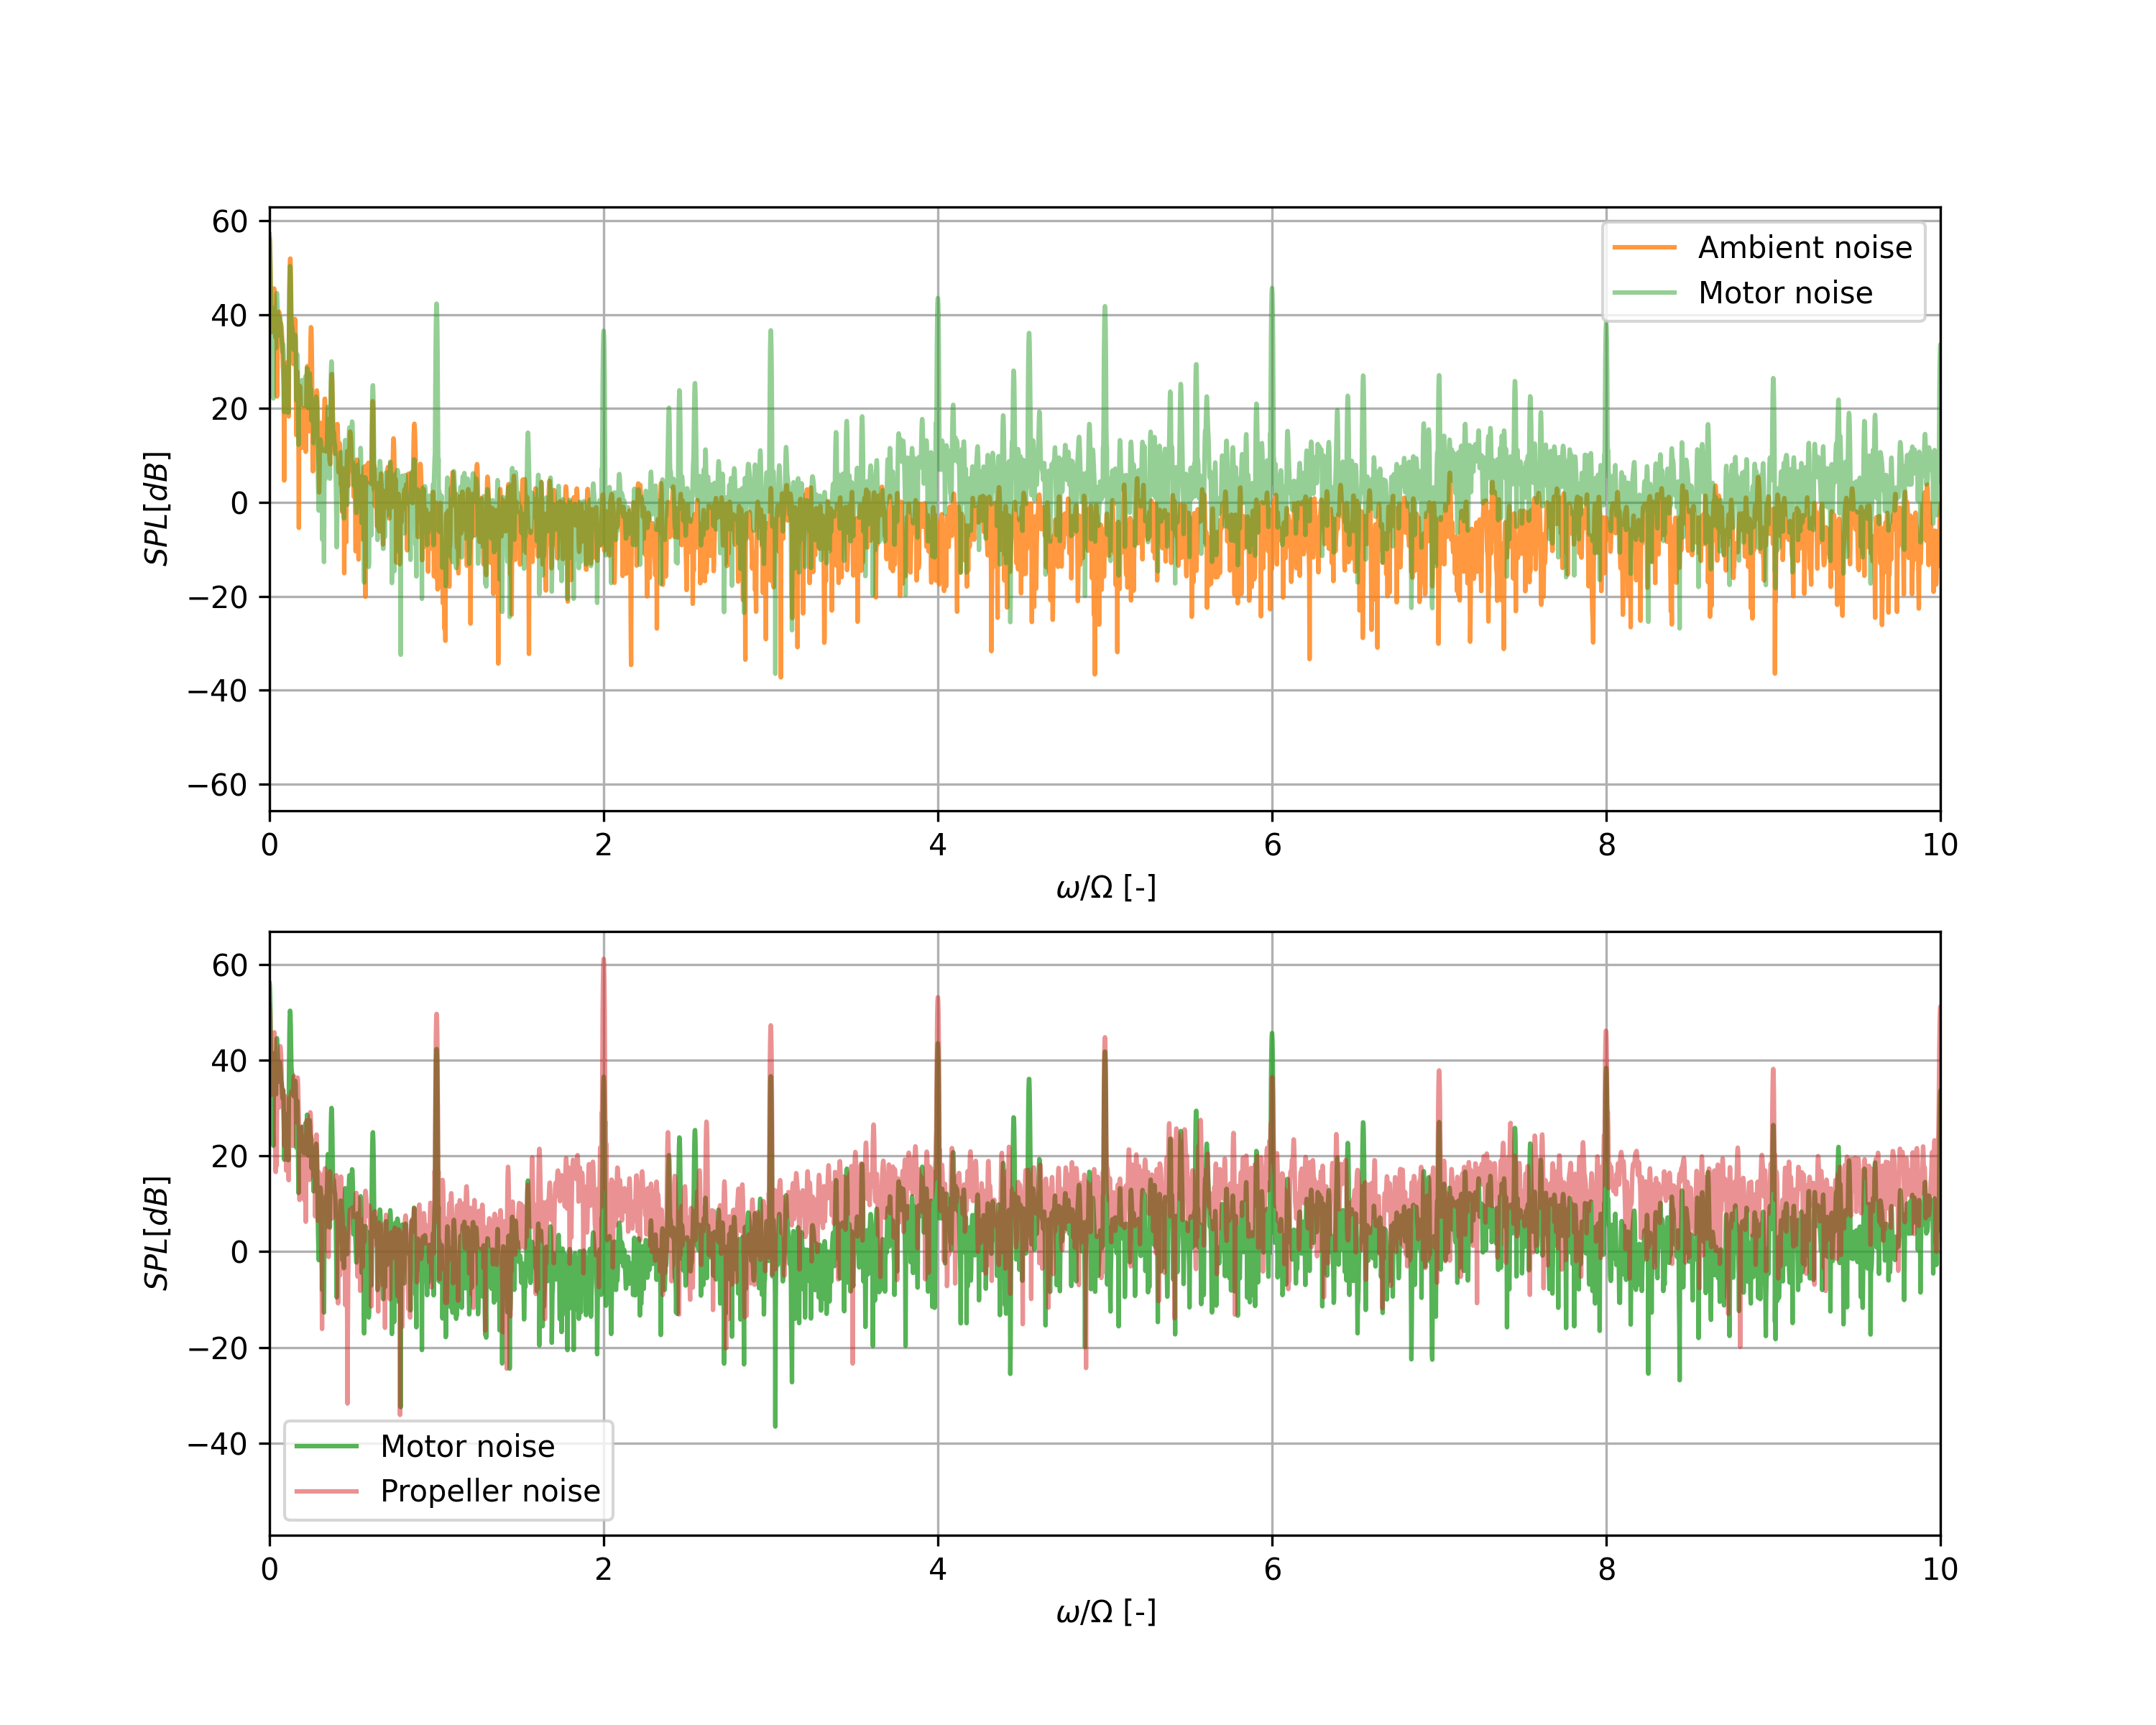
\includegraphics[width=0.8\textwidth]{../figures/spectrum_plot.pdf}
    \caption{Spectrum of the dalprop 5045 propeller at 12000 RPM.}
    \label{fig:propeller_spectrum}
\end{figure}

Figure \ref{fig:propeller_spectrum} shows a typical SPL spectrum with its frequency normalised by the rotation speed.
Peaks can be seen at integers of the blade speed frequency, with significant peaks at multiples of the blade number 2.
Motor noise typically has a significant tone at a multiple of its pole pair count, which is 7 for the motor used \cite{motor_vibration}.
However, no signficant peak is observed, suggesting that the FOC algorithm used to drive the motor has reduced the noise \cite{en13102534}.
The propeller noise has a broadband ~10dB above that of the motor, with some harmonics being 20dB above the motor noise.
The 6th speed, or 3rd harmonic of blade passage frequency shows a reduced sound pressure level compared to the motor noise.
This demonstrates destructive interference between the motor noise and the propeller noise at this frequency.

\begin{figure}[H]
    \centering
    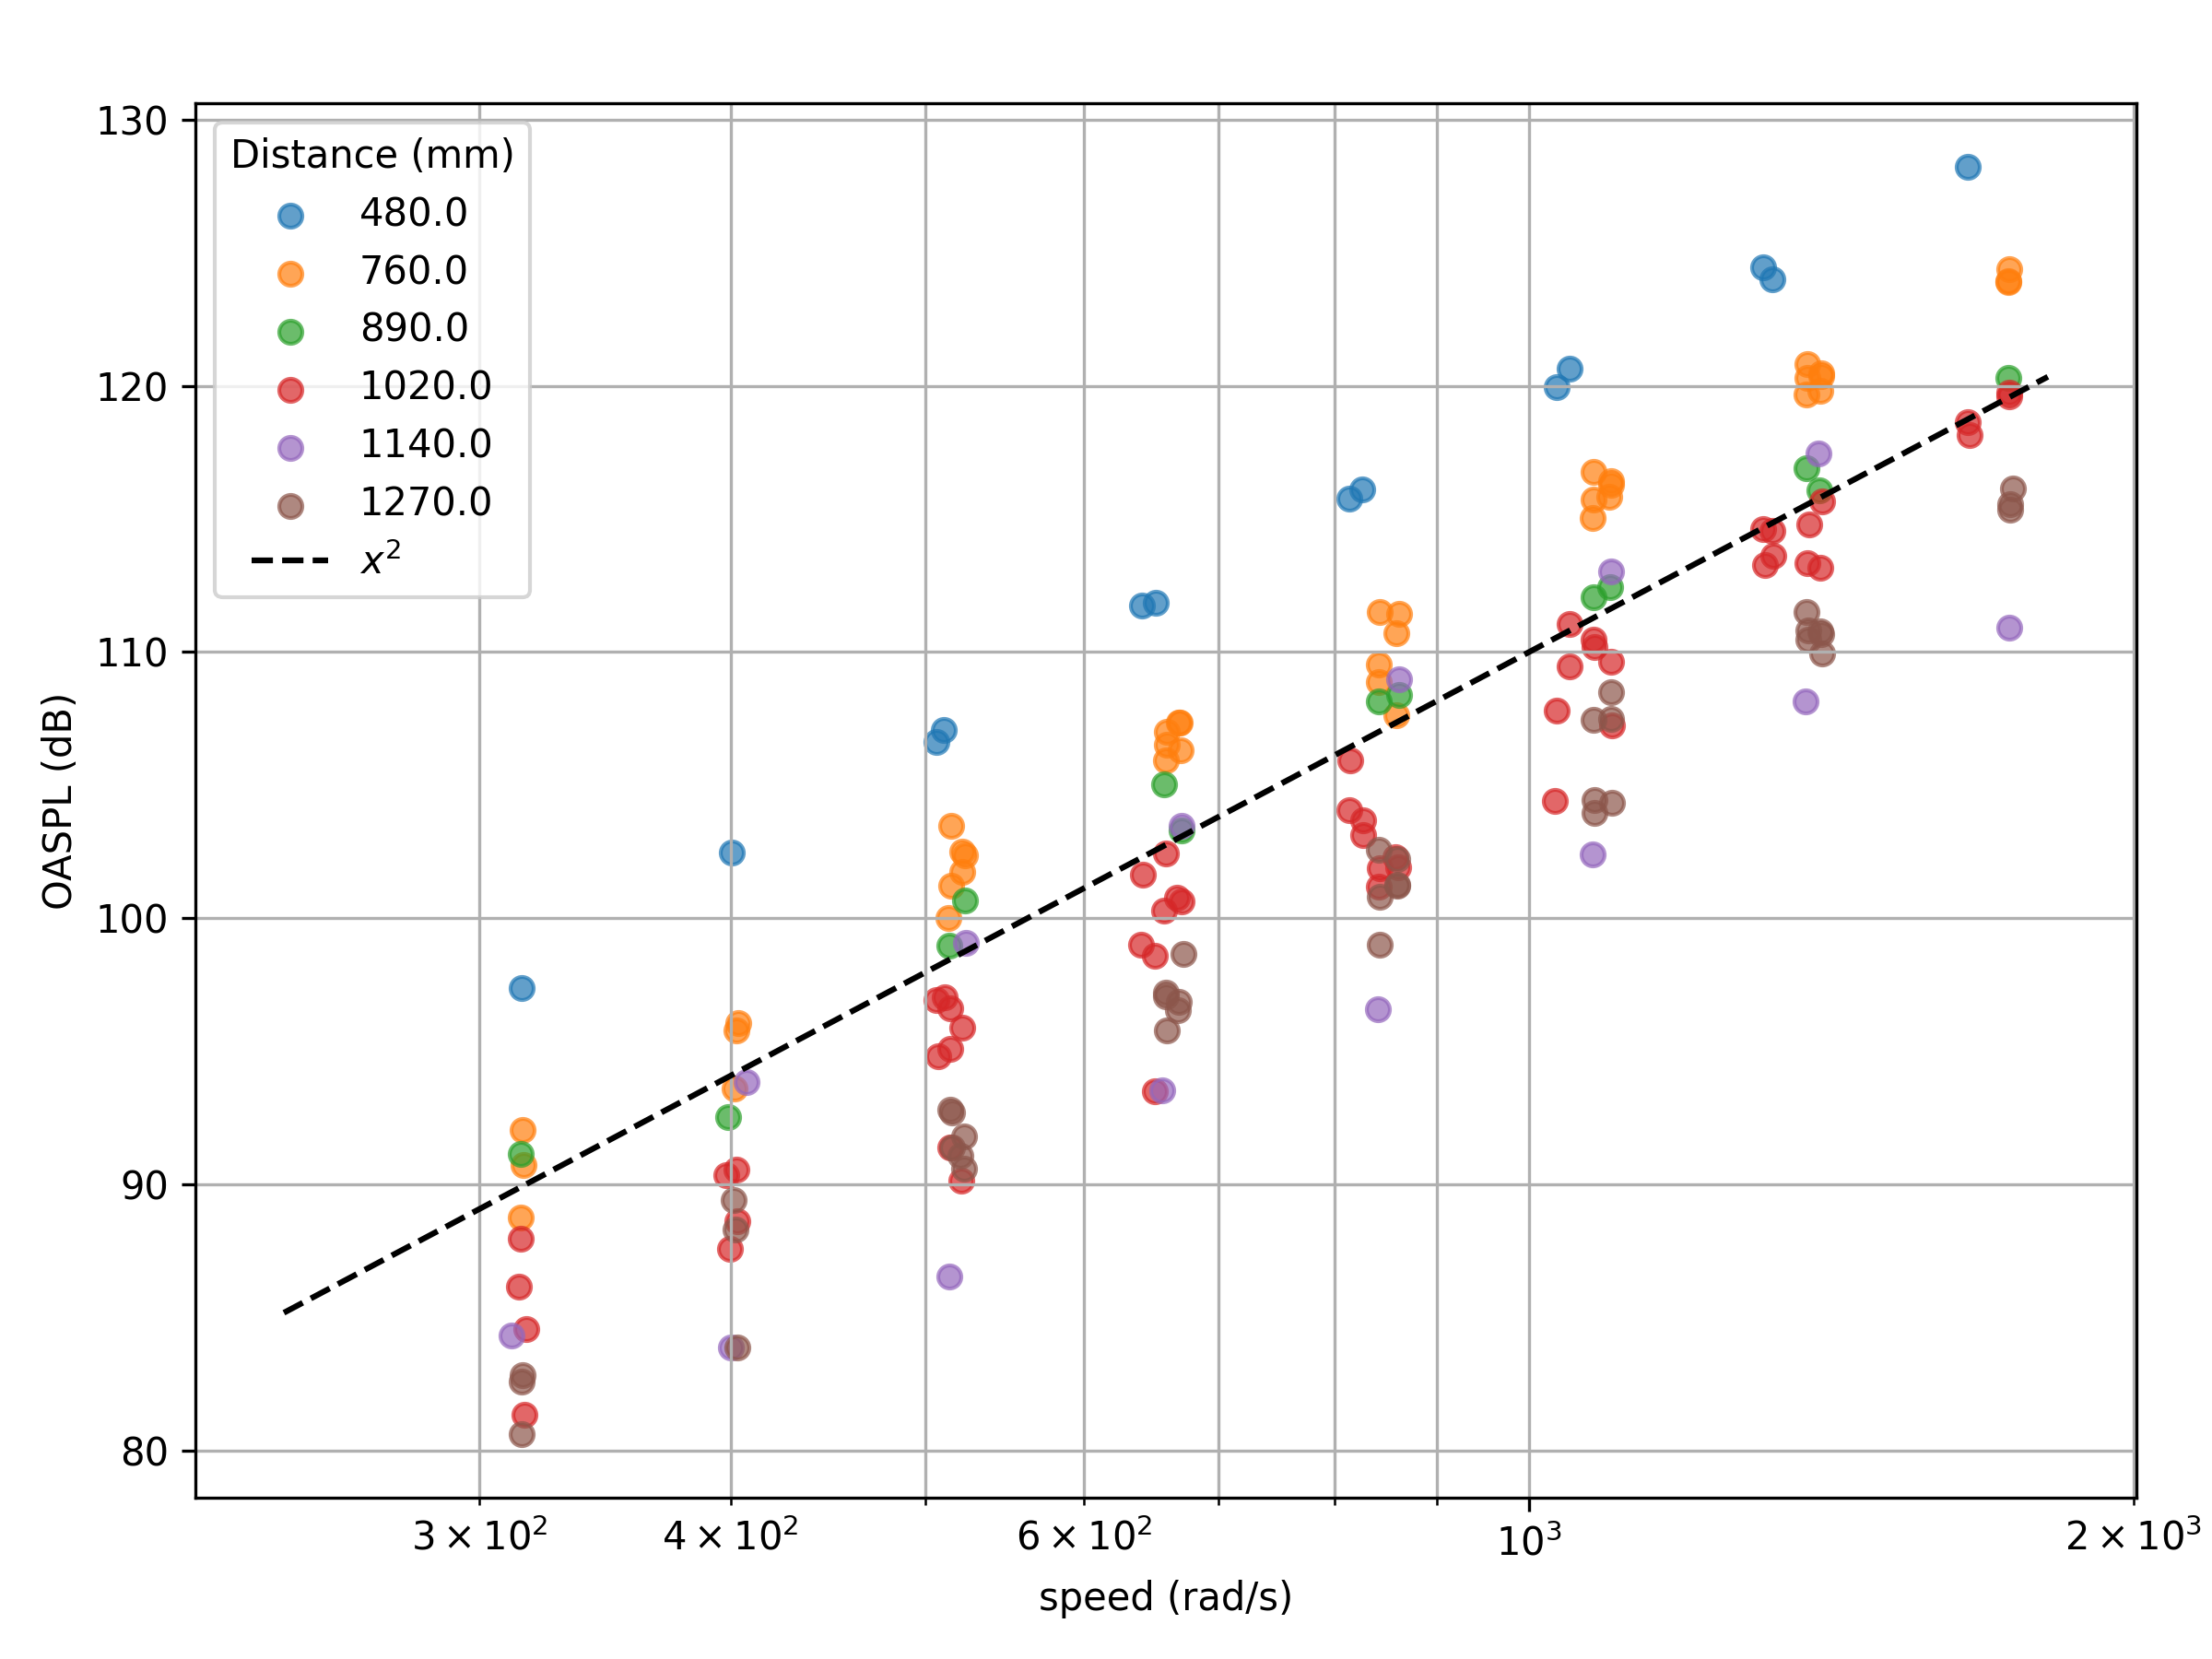
\includegraphics[width=0.8\textwidth]{../figures/spl_speed_variation.pdf}
    \caption{OASPL of the dalprop 5045 propeller }
    \label{fig:spl_speed_variation}
\end{figure}

Figure \ref{fig:spl_speed_variation} shows OASPL against speed at $\theta = 180^\circ$ for the dalprop 5045 propeller.
An obvious square power law can be seen from the data, with OASPL also increasing with decreasing distance.
The distance 18.1 blade radii shows audio data that was indexed ahead of the motor data, which was meant to be corrected for,
However, in this case it was 2 indexes ahead and so went unnoticed.

\begin{figure}[H]
    \centering
    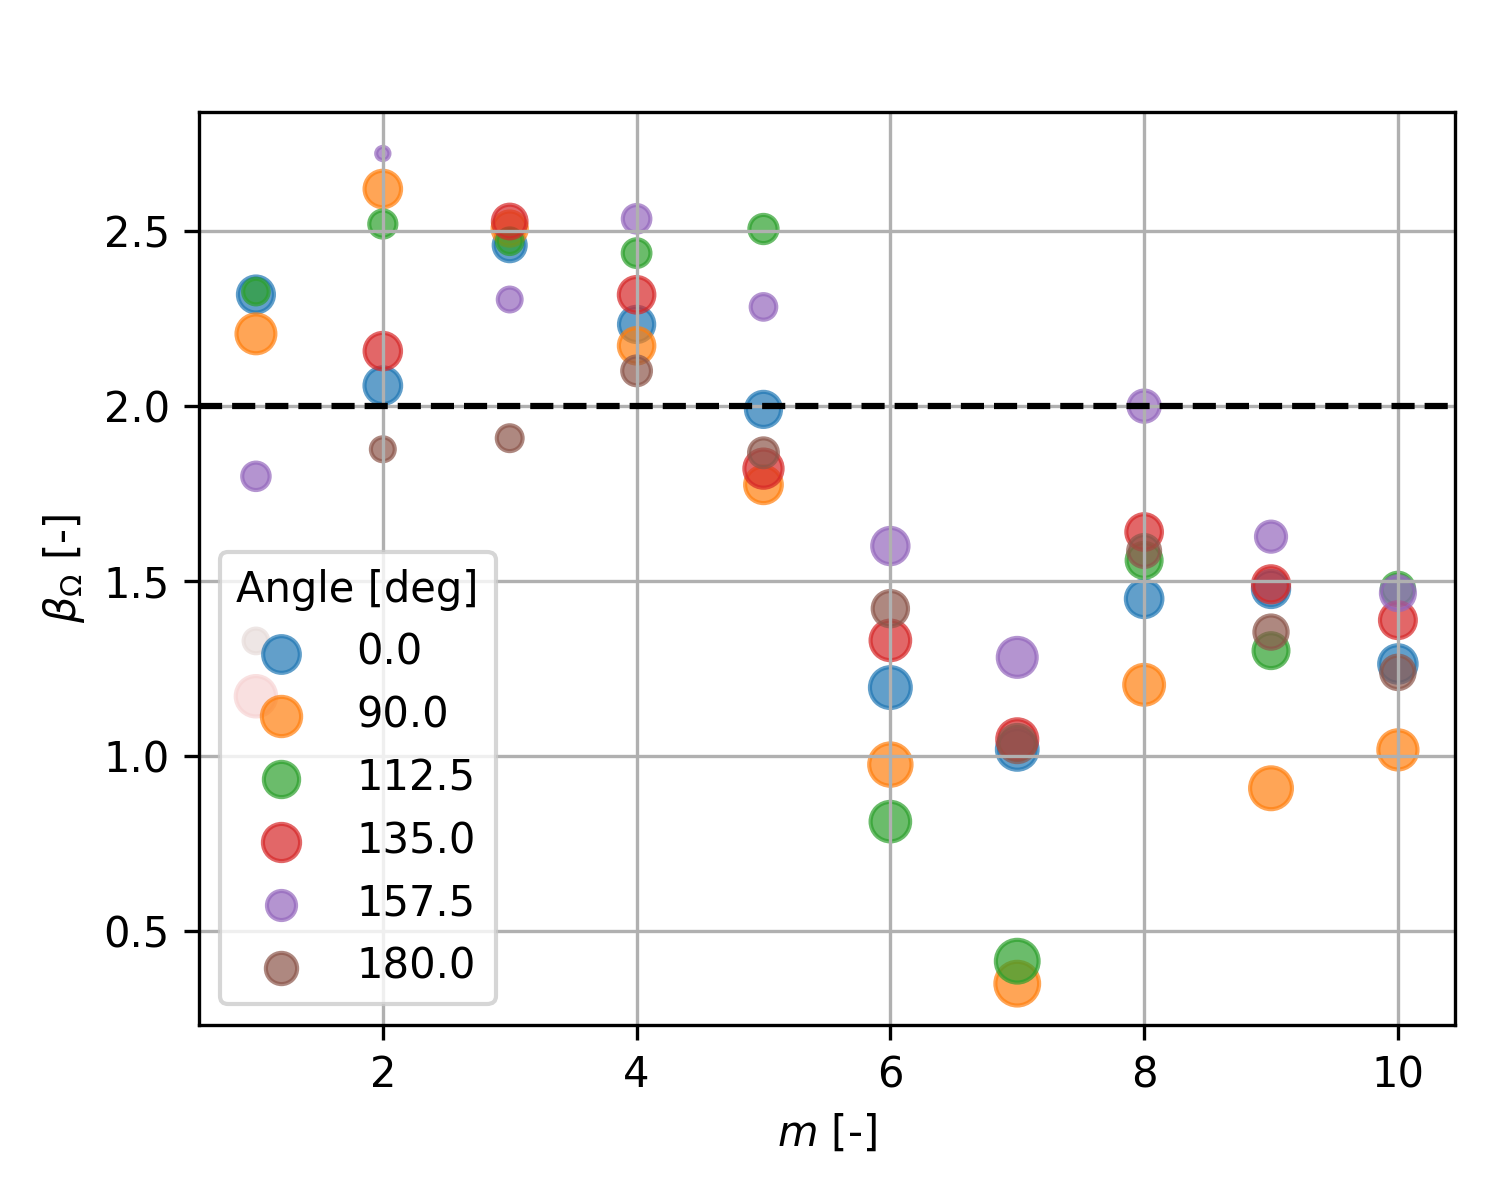
\includegraphics[width=0.8\textwidth]{../figures/speed_coefficient_for_angles_harmonics.pdf}
    \caption{Speed coefficient}
    \label{fig:speed_coefficient_for_angles_harmonics}
        
    \caption{Power law coefficients for various observer angles and harmonics for the dalprop 5045 propeller.}
\end{figure}

Figures \ref{fig:speed_coefficient_for_angles_harmonics} and \ref{fig:distance_coefficient_for_angles_harmonics} 
show the respective fitted power law coefficients for speed and distance for the dalprop 5045 propeller.
They are plotted against the harmonic number, with colour representing the angle of the observer.
The size of the marker represents the relative standard deviation of the residual.

At low harmonics, the speed coefficient is close to the expected value of 2 for many angles.
The angle of 157.5 degrees shows a small deviation in residuals, indicating a relatively strong fit, and the highest 
dependence on speed.
This must be due to increased constructive interference occuring at higher speeds
At higher harmonics the coefficient decreases below 2 for all angles indicating destructive interference.
Another observation is that at higher harmonics, there is typically higher variation in the residuals, indicating a worse fit.
This worse fit could be due to speed or distance dependence.

\begin{figure}[H]
    \centering
    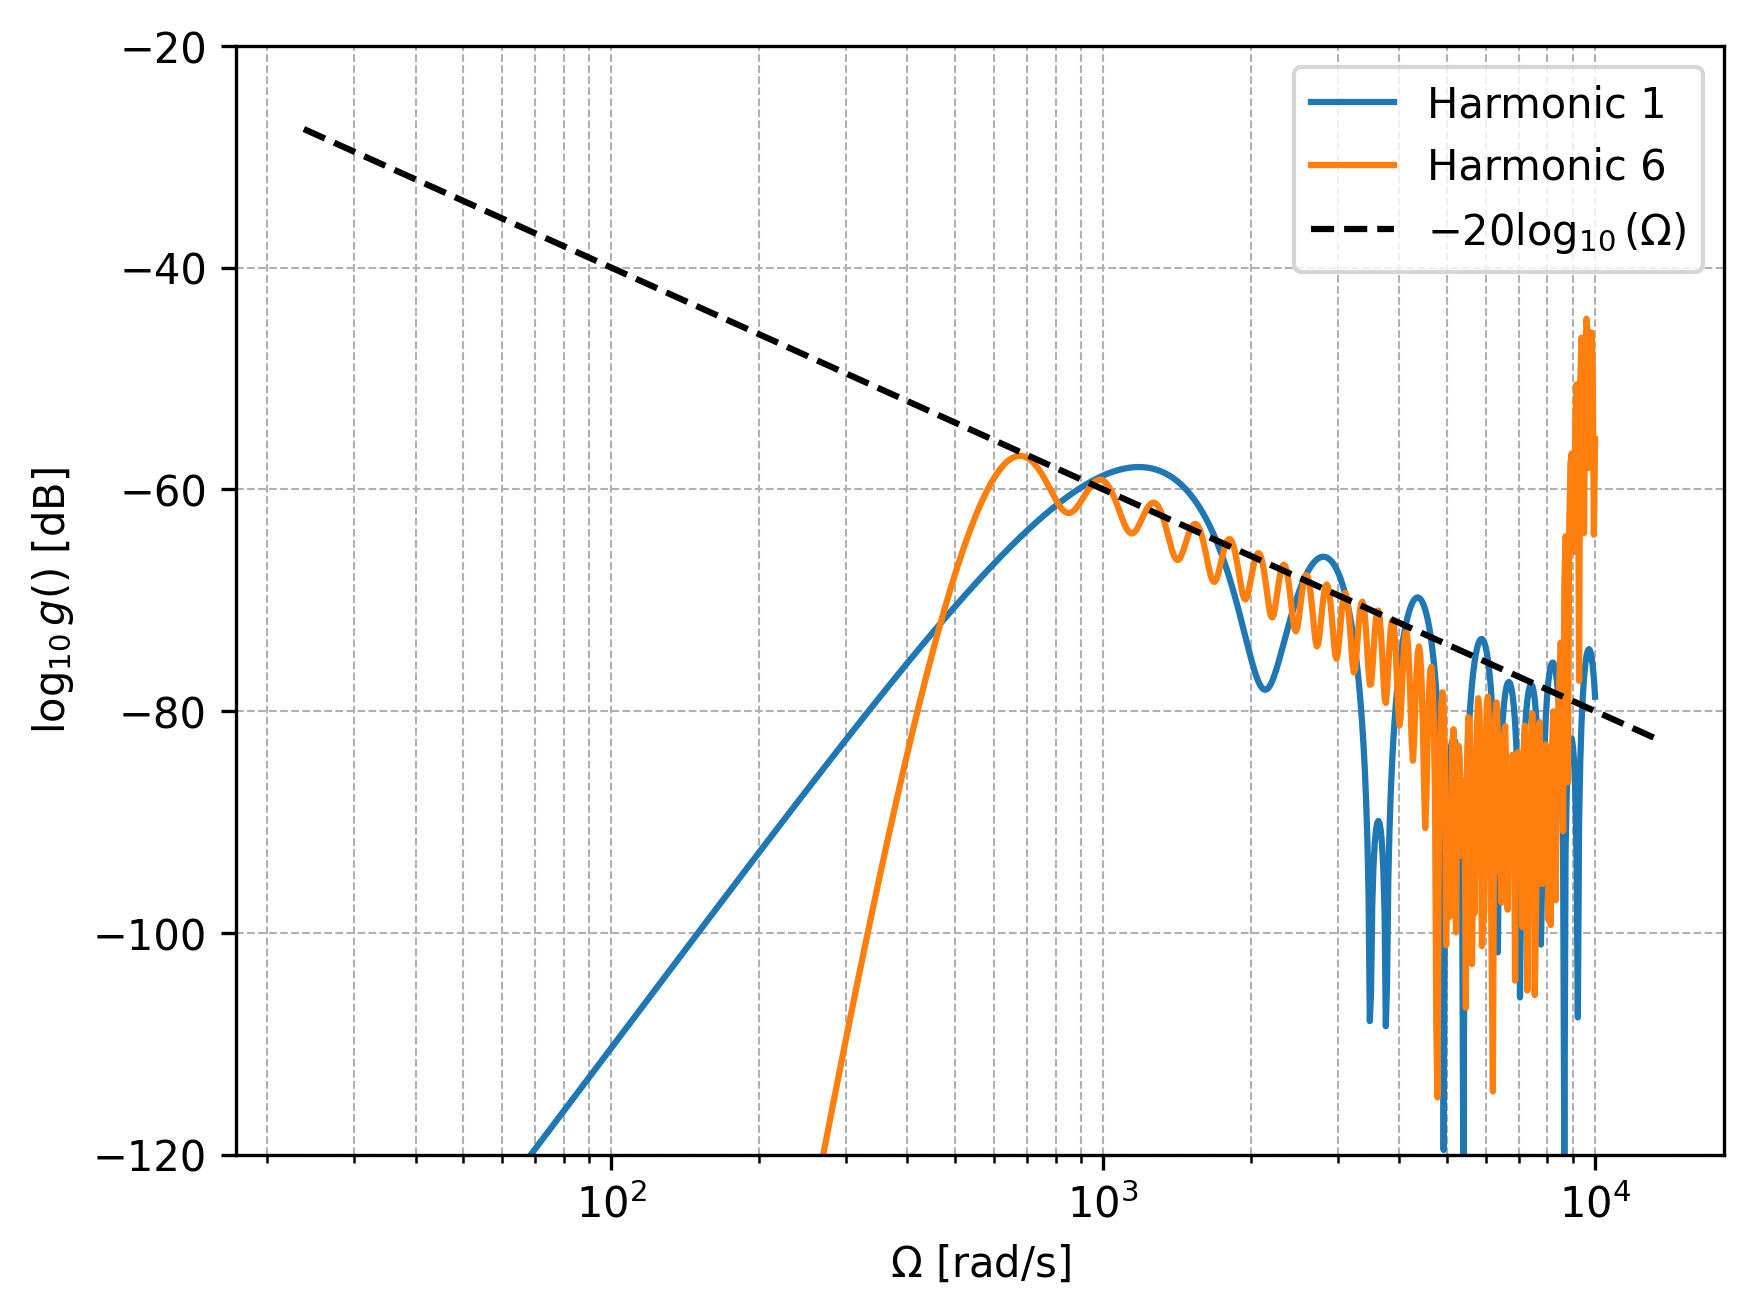
\includegraphics[width=0.8\textwidth]{../figures/hanson_speed_dependence.pdf}
    \caption{Interference factor $g$ derived from Hanson's theory against speed for harmonics 1 and 6}
    \label{fig:hanson_speed_dependence}
\end{figure}

Figure \ref{fig:hanson_speed_dependence} shows the function $g$ derived from Hansons theory gainst speed for an observer at $\theta = 135^\circ$.
The speed dependence shows an initially strong positive dependence on speed, before decreasing to an inverse dependence.
The speed at which the transition occurs reduces with increasing harmonic number.
This is thought to explain the overshoot in speed coefficient at low harmonics shown in figure \ref{fig:speed_coefficient_for_angles_harmonics}.
This also explains the subsequent decrease at higher harmonics as the fit is dominated by the negative speed dependence.
The high frequency part of the graph is due to a lack of spanwise resolution in the integration.
The dependence of the interference factor on speed reduces the suitability of the comparative metric.

\begin{figure}[H]
    \centering
    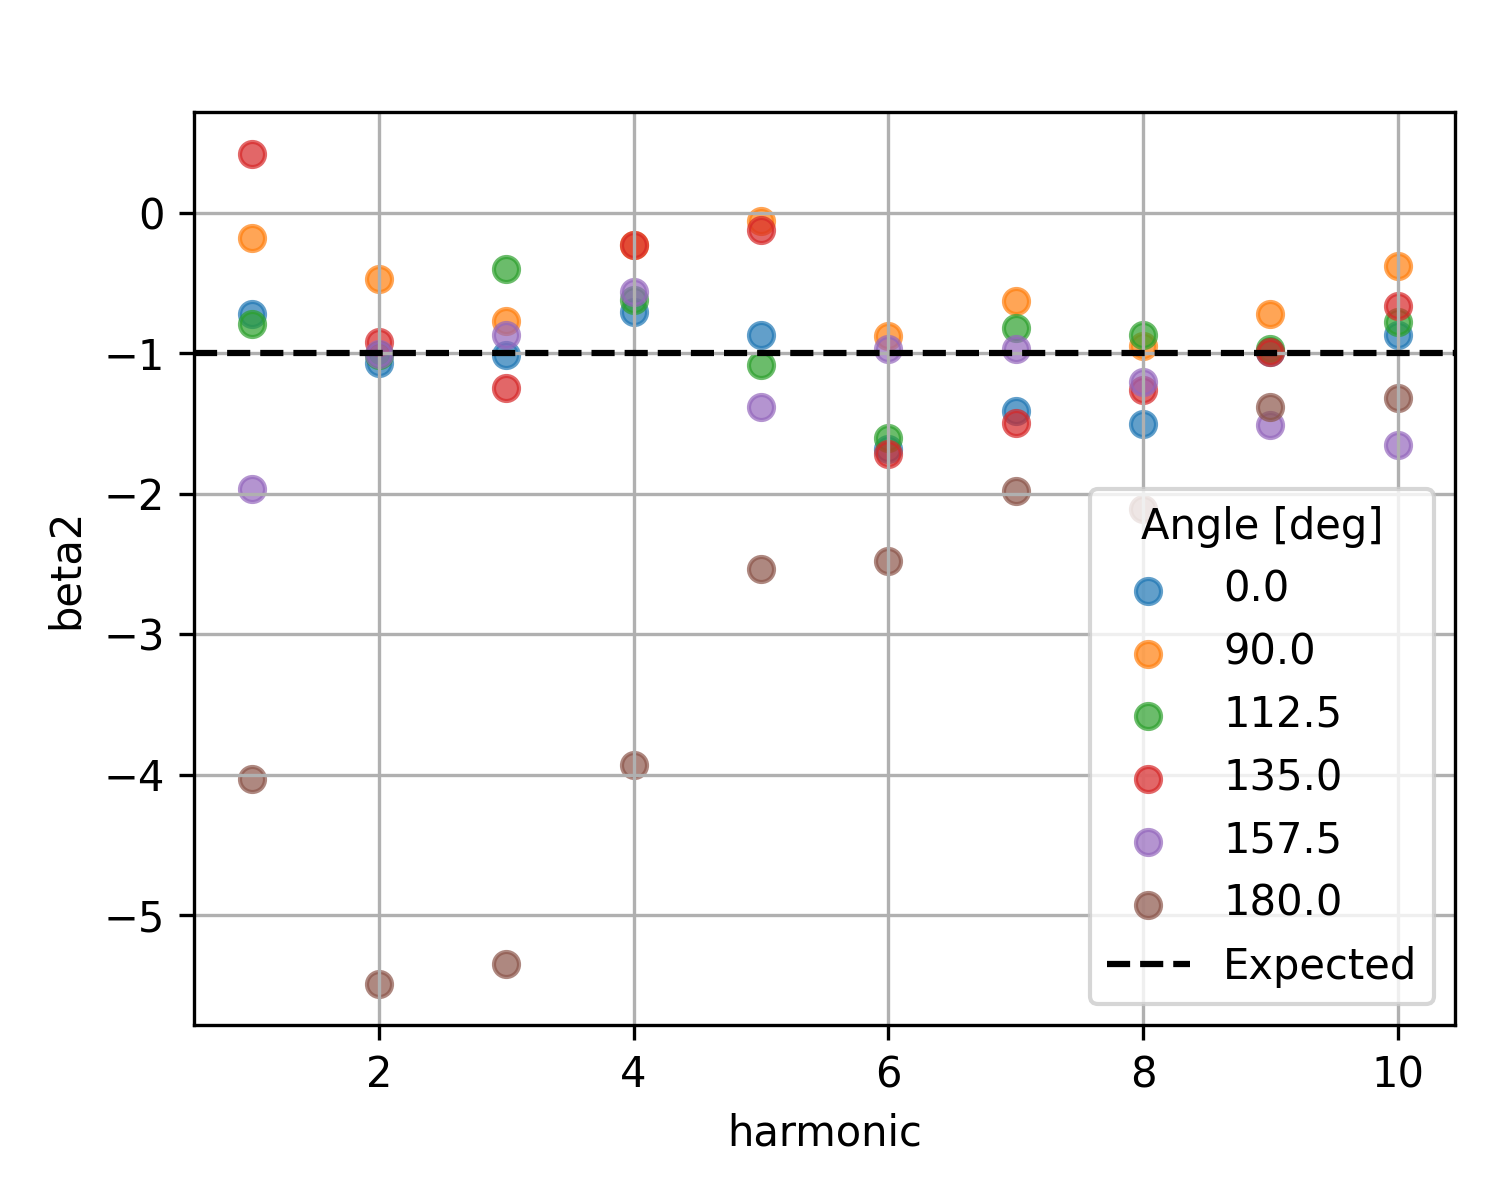
\includegraphics[width=0.8\textwidth]{../figures/distance_coefficient_for_angles_harmonics.pdf}
    \caption{Distance coefficient}
    \label{fig:distance_coefficient_for_angles_harmonics}
\end{figure}

The distance coefficients in figure \ref{fig:distance_coefficient_for_angles_harmonics} are shown to be negative for nearly all angles and harmonics but varies significantly.
This is partly due to the narrow range and number of observer distances tested.

At $\theta=180^\circ$, the microphone is in the propeller wake where the sound is dominated by turbulent velocity, known to be an 8th power law \cite{lighthill_1952}.
The strongly negative distance coefficient shown in figure \ref{fig:distance_coefficient_for_angles_harmonics} is due to both this and the turbulent wake velocity distance dependence.


% size of harmonics becoming insignificant?


\begin{figure}[H]
    \centering
    \begin{subfigure}[t]{0.49\textwidth}
        \centering
        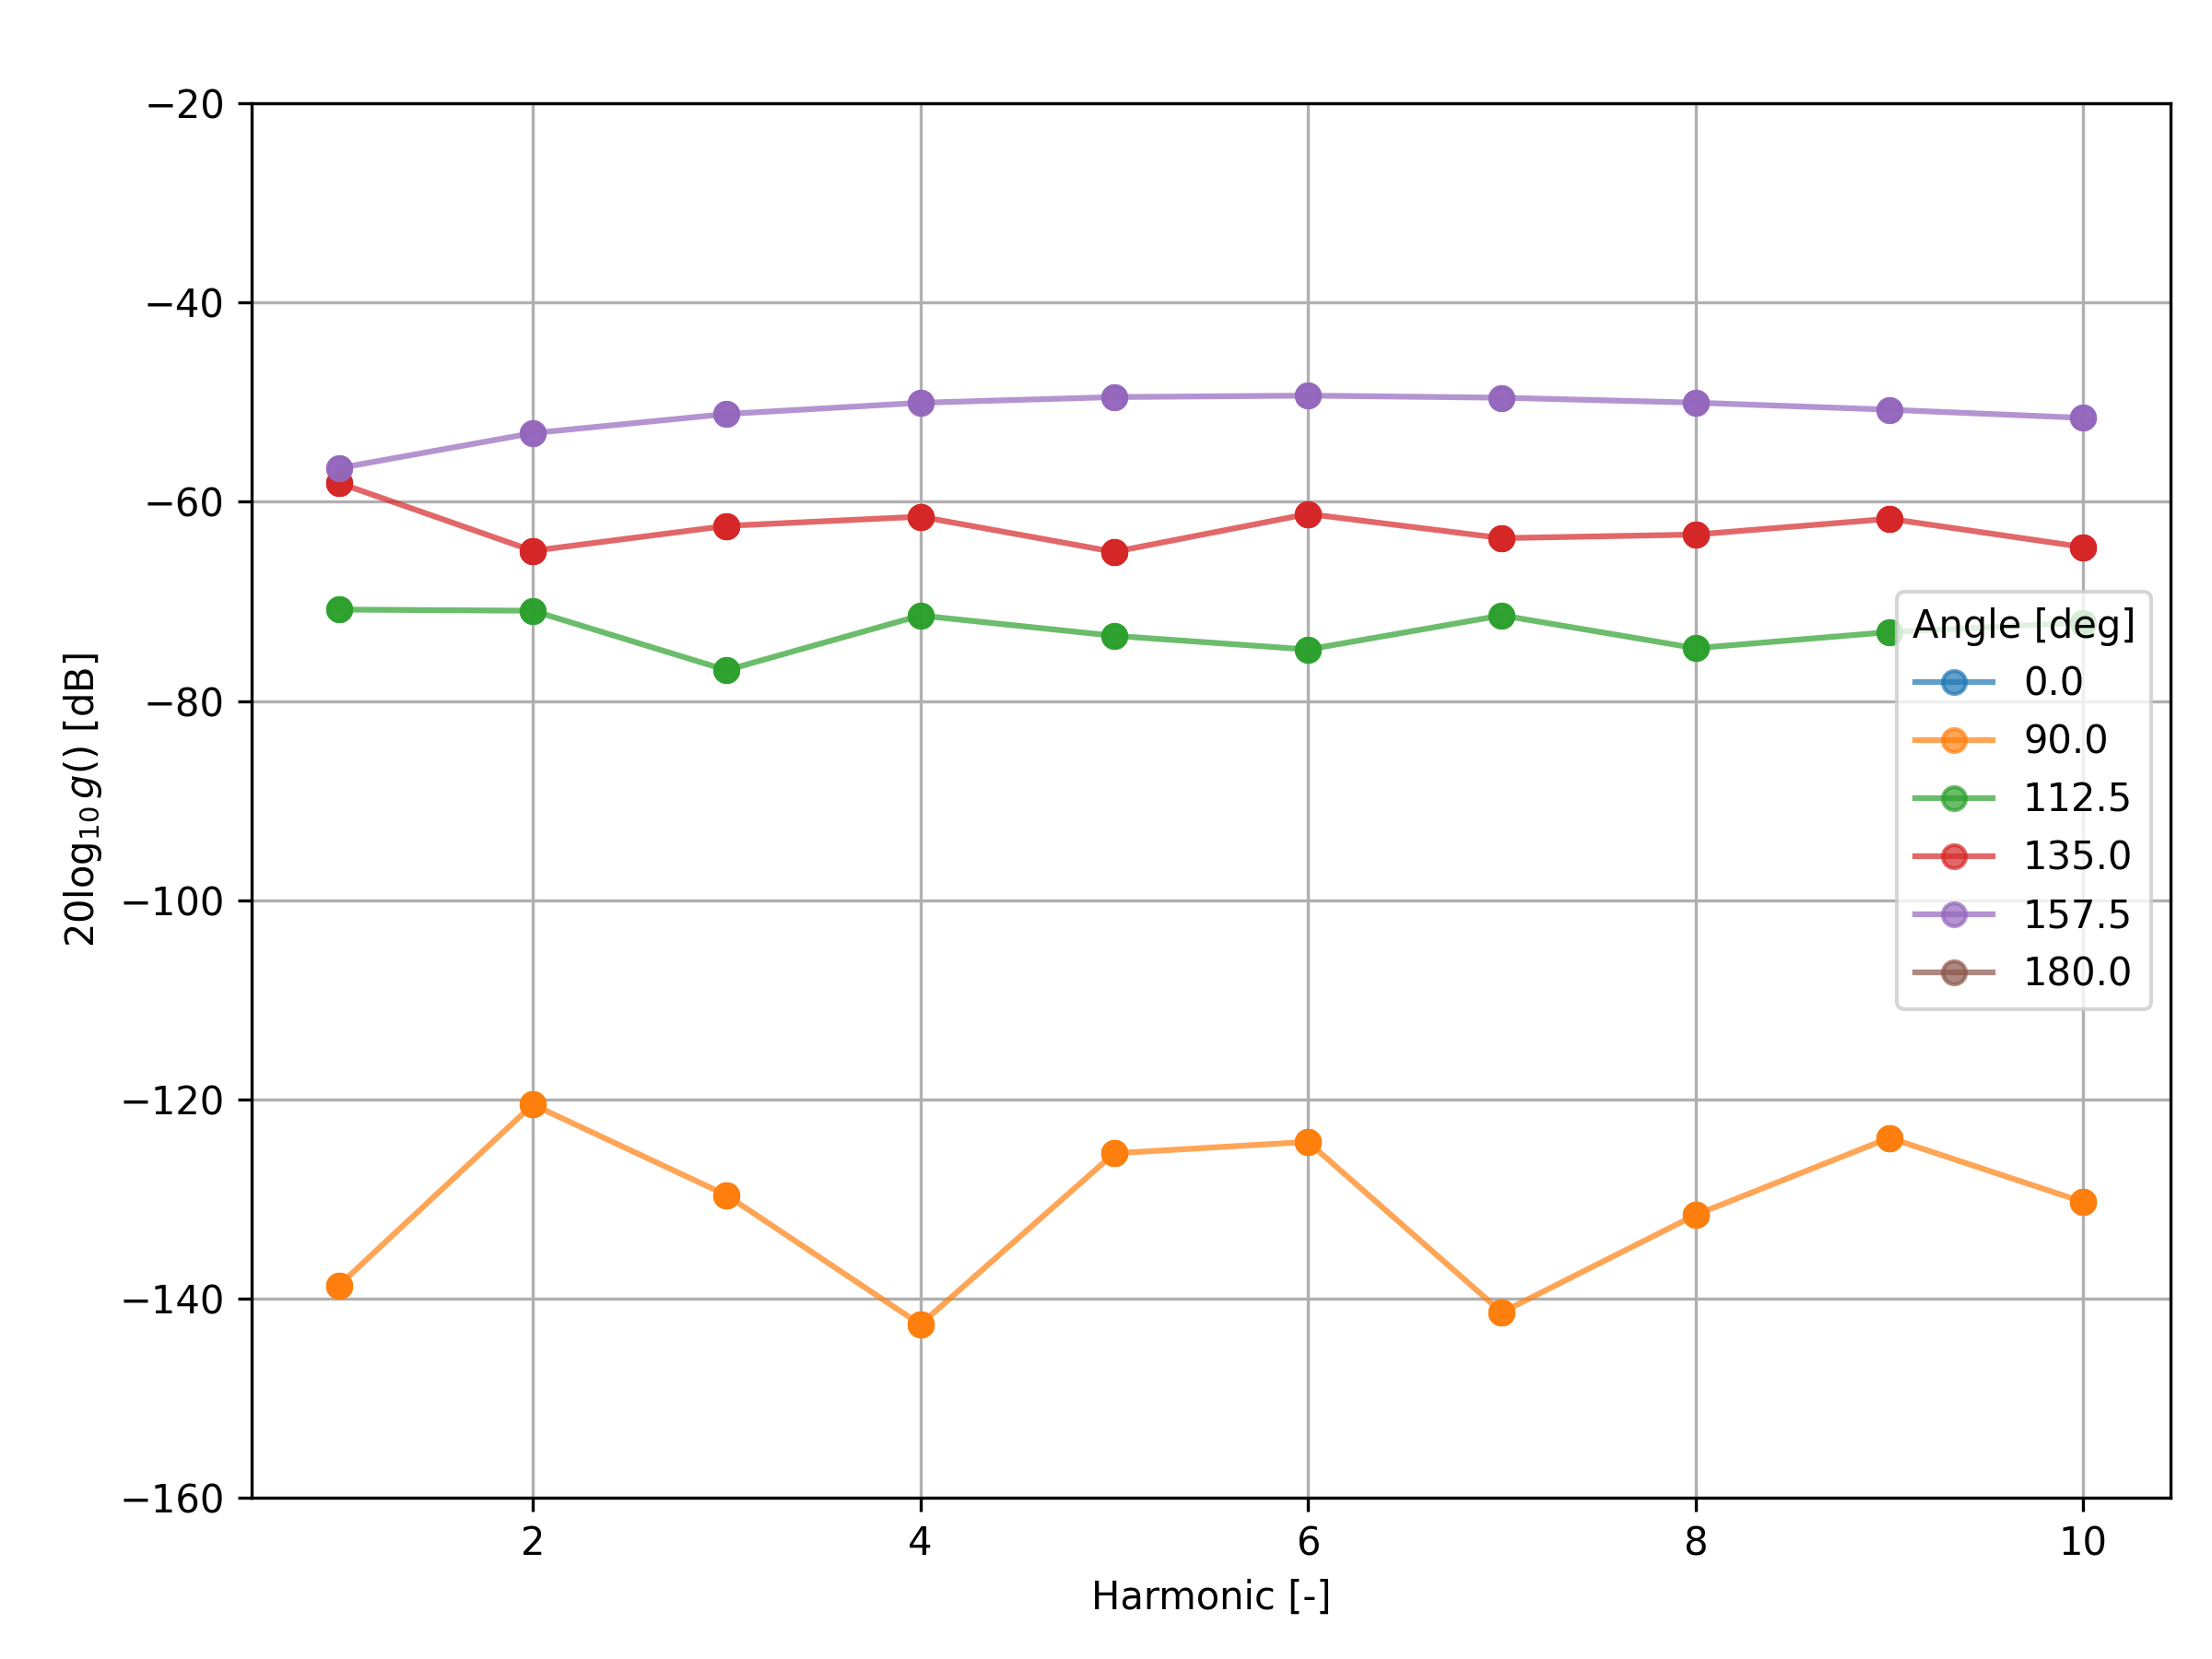
\includegraphics[width=\textwidth]{../figures/harmonic_hanson_angle_for_dalprop5045.pdf}
        \caption{Theoretical}
        \label{fig:harmonic_hanson_angle_for_dalprop5045}
    \end{subfigure}
    \begin{subfigure}[t]{0.49\textwidth}
        \centering
        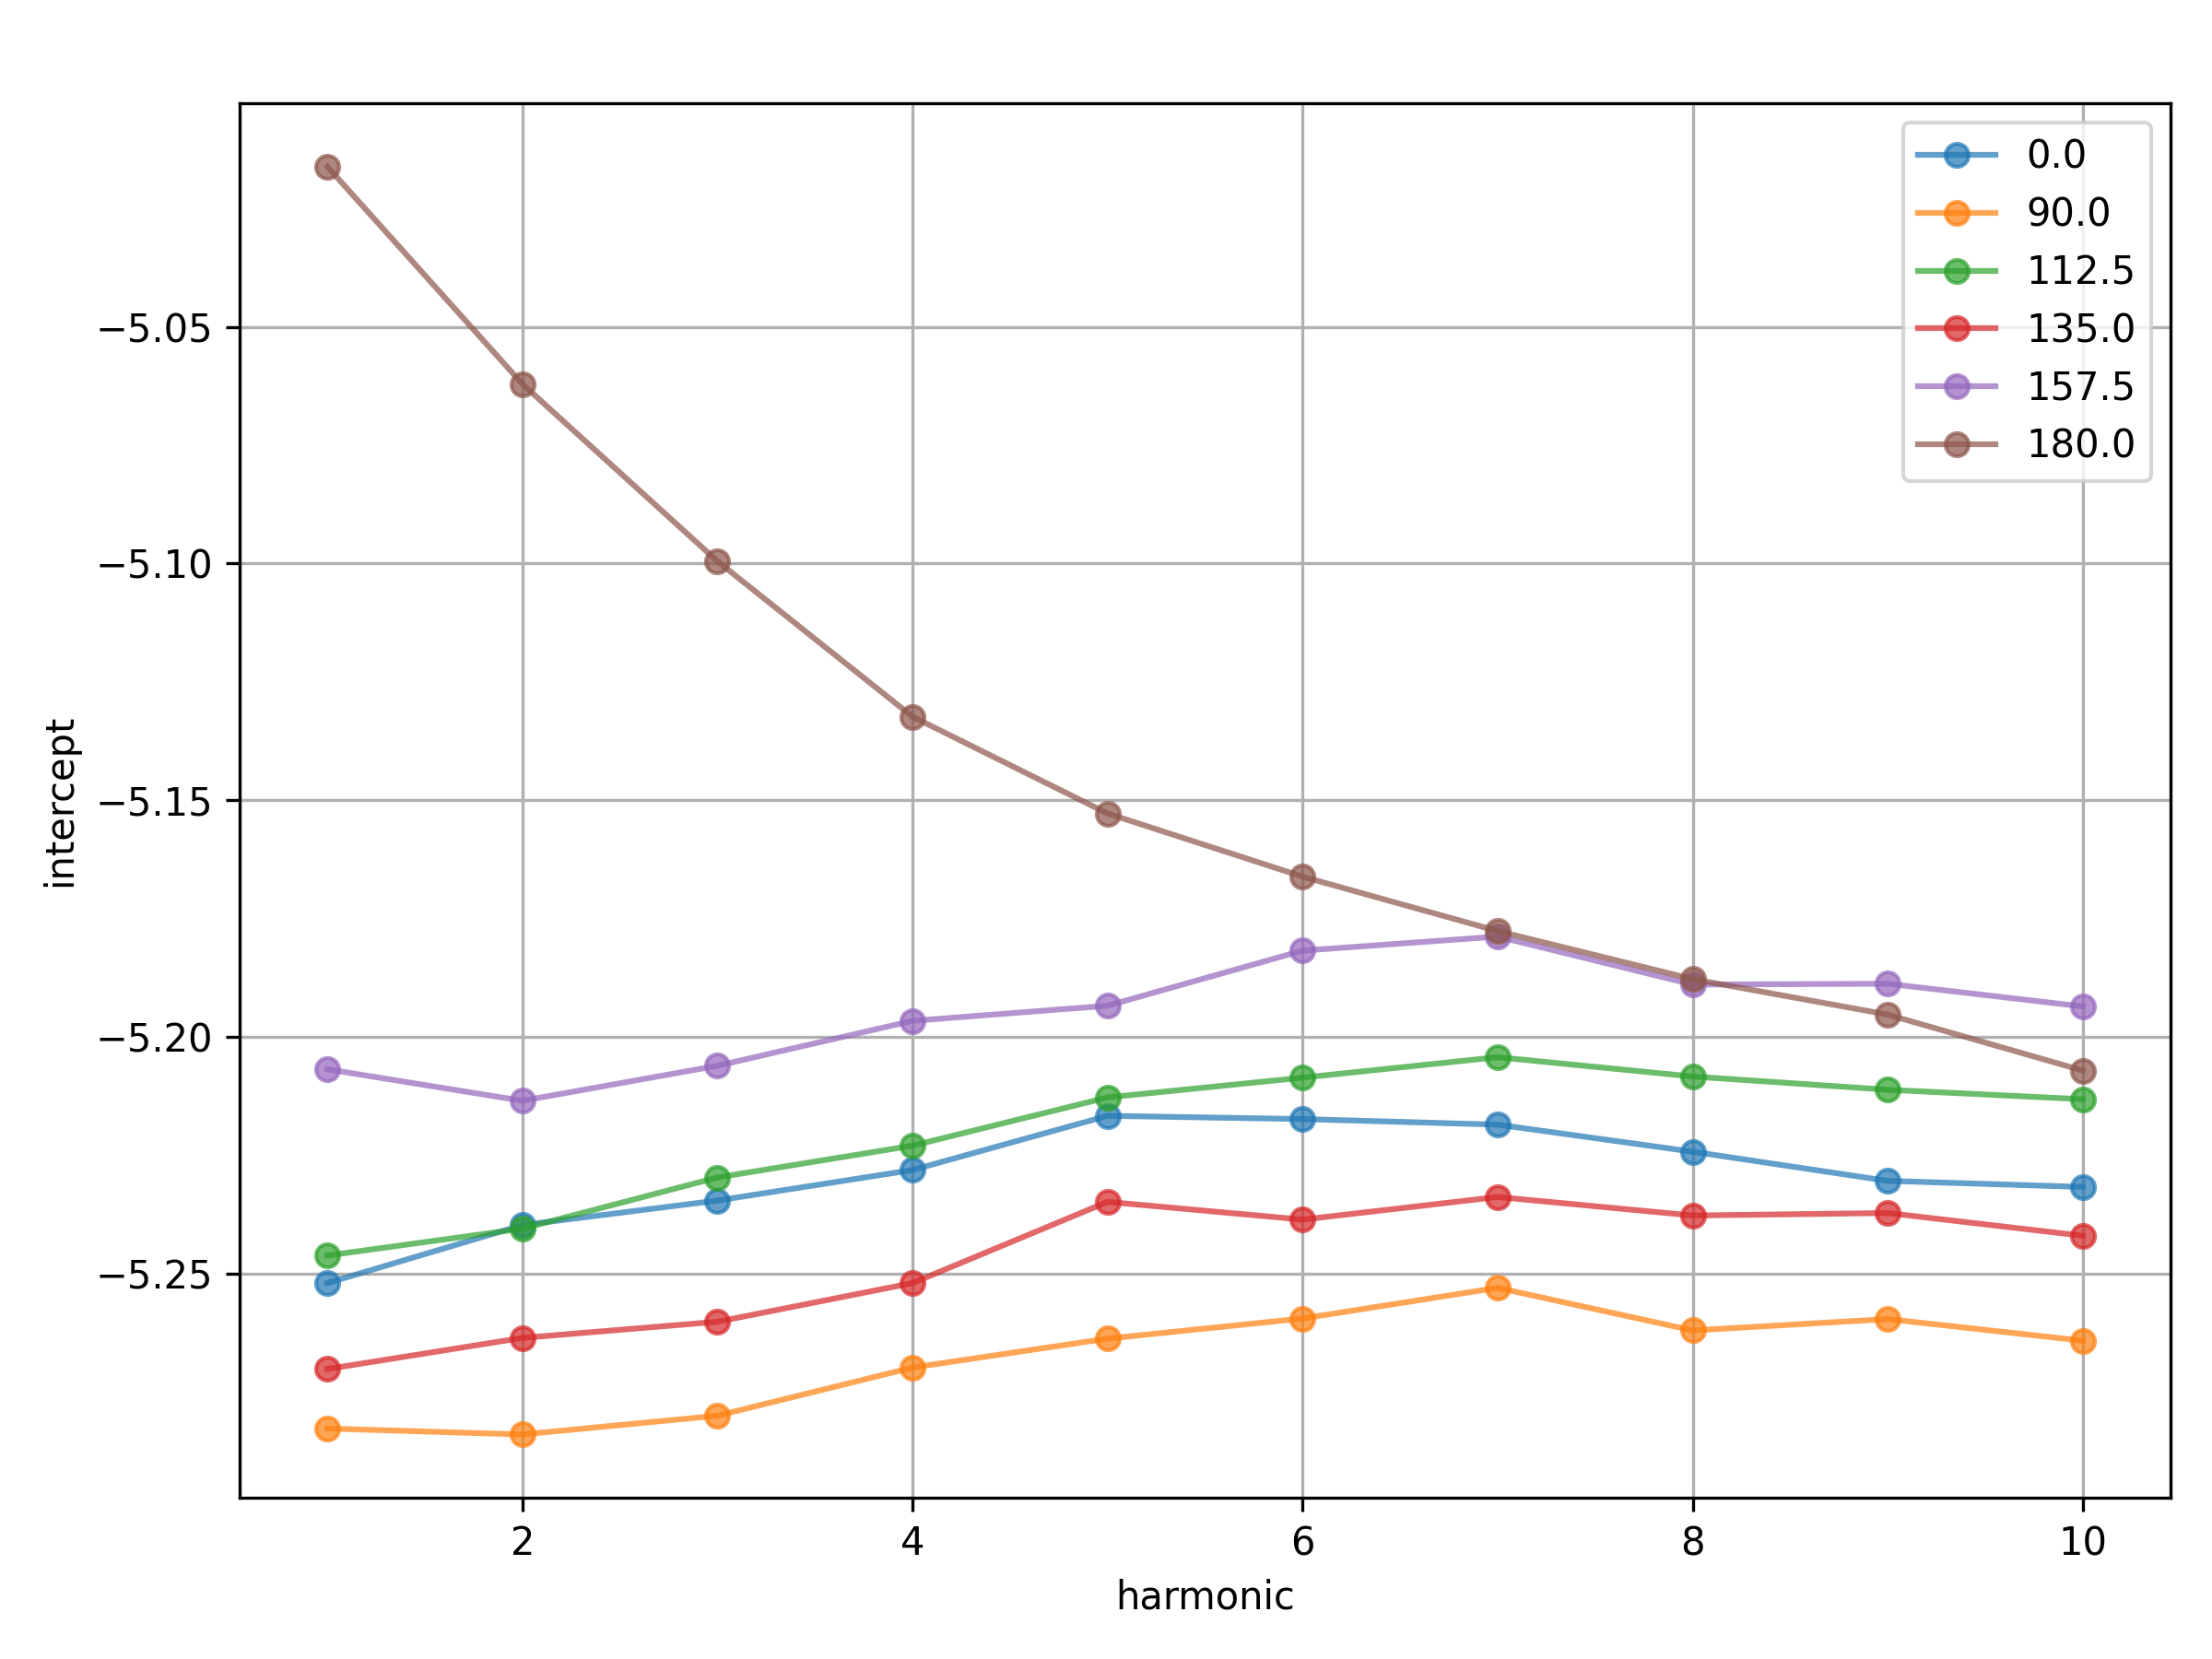
\includegraphics[width=\textwidth]{../figures/harmonic_sound_angle_for_dalprop5045.pdf}
        \caption{Experimental}
        \label{fig:harmonic_sound_angle_for_dalprop5045}
    \end{subfigure}
    \caption{Theoretical and experimental harmonic interference for the dalprop5045 at different observer angles.}
\end{figure}

Figures \ref{fig:harmonic_hanson_angle_for_dalprop5045} and \ref{fig:harmonic_sound_angle_for_dalprop5045} show the theoretical and experimental harmonic interference for the dalprop 5045 propeller at different observer angles.
Theory predicts the harmonic noise at $\theta=180^\circ$ and $0^\circ$ to be negligible, which is why these are not seen in figure \ref{fig:harmonic_hanson_angle_for_dalprop5045}.
The experimental results show a strong presence of noise at $180^\circ$, which could be due to turbulence from the propeller not accounted for in the theory.
However, as discussed previously, the noise on this microphone is thought to be dominated by the turbulent wake itself.
The noise at $0^\circ$ is also seen in the experimental results to be significant in magnitude, differing from theory, which is not understood.
The theoretical results and experimental results agree that noise at all harmonics and the angle $157.5^\circ$ are the highest, ignoring the $180^\circ$ and $0^\circ$ angles.
It also agrees that the noise at $90^\circ$ is the lowest.
Theory finds the noise at $135^\circ$ to be higher than that at $112.5^\circ$ but the experimental results show the opposite.
Another observation is that the experimental results show a decreasing trend in noise with increasing harmonic number.
The reason for this is also not understood, as it cant be due to broadband. It could however be due to interference from another noise source.

\begin{figure}[H]
    \centering
    \begin{subfigure}[t]{0.49\textwidth}
        \centering
        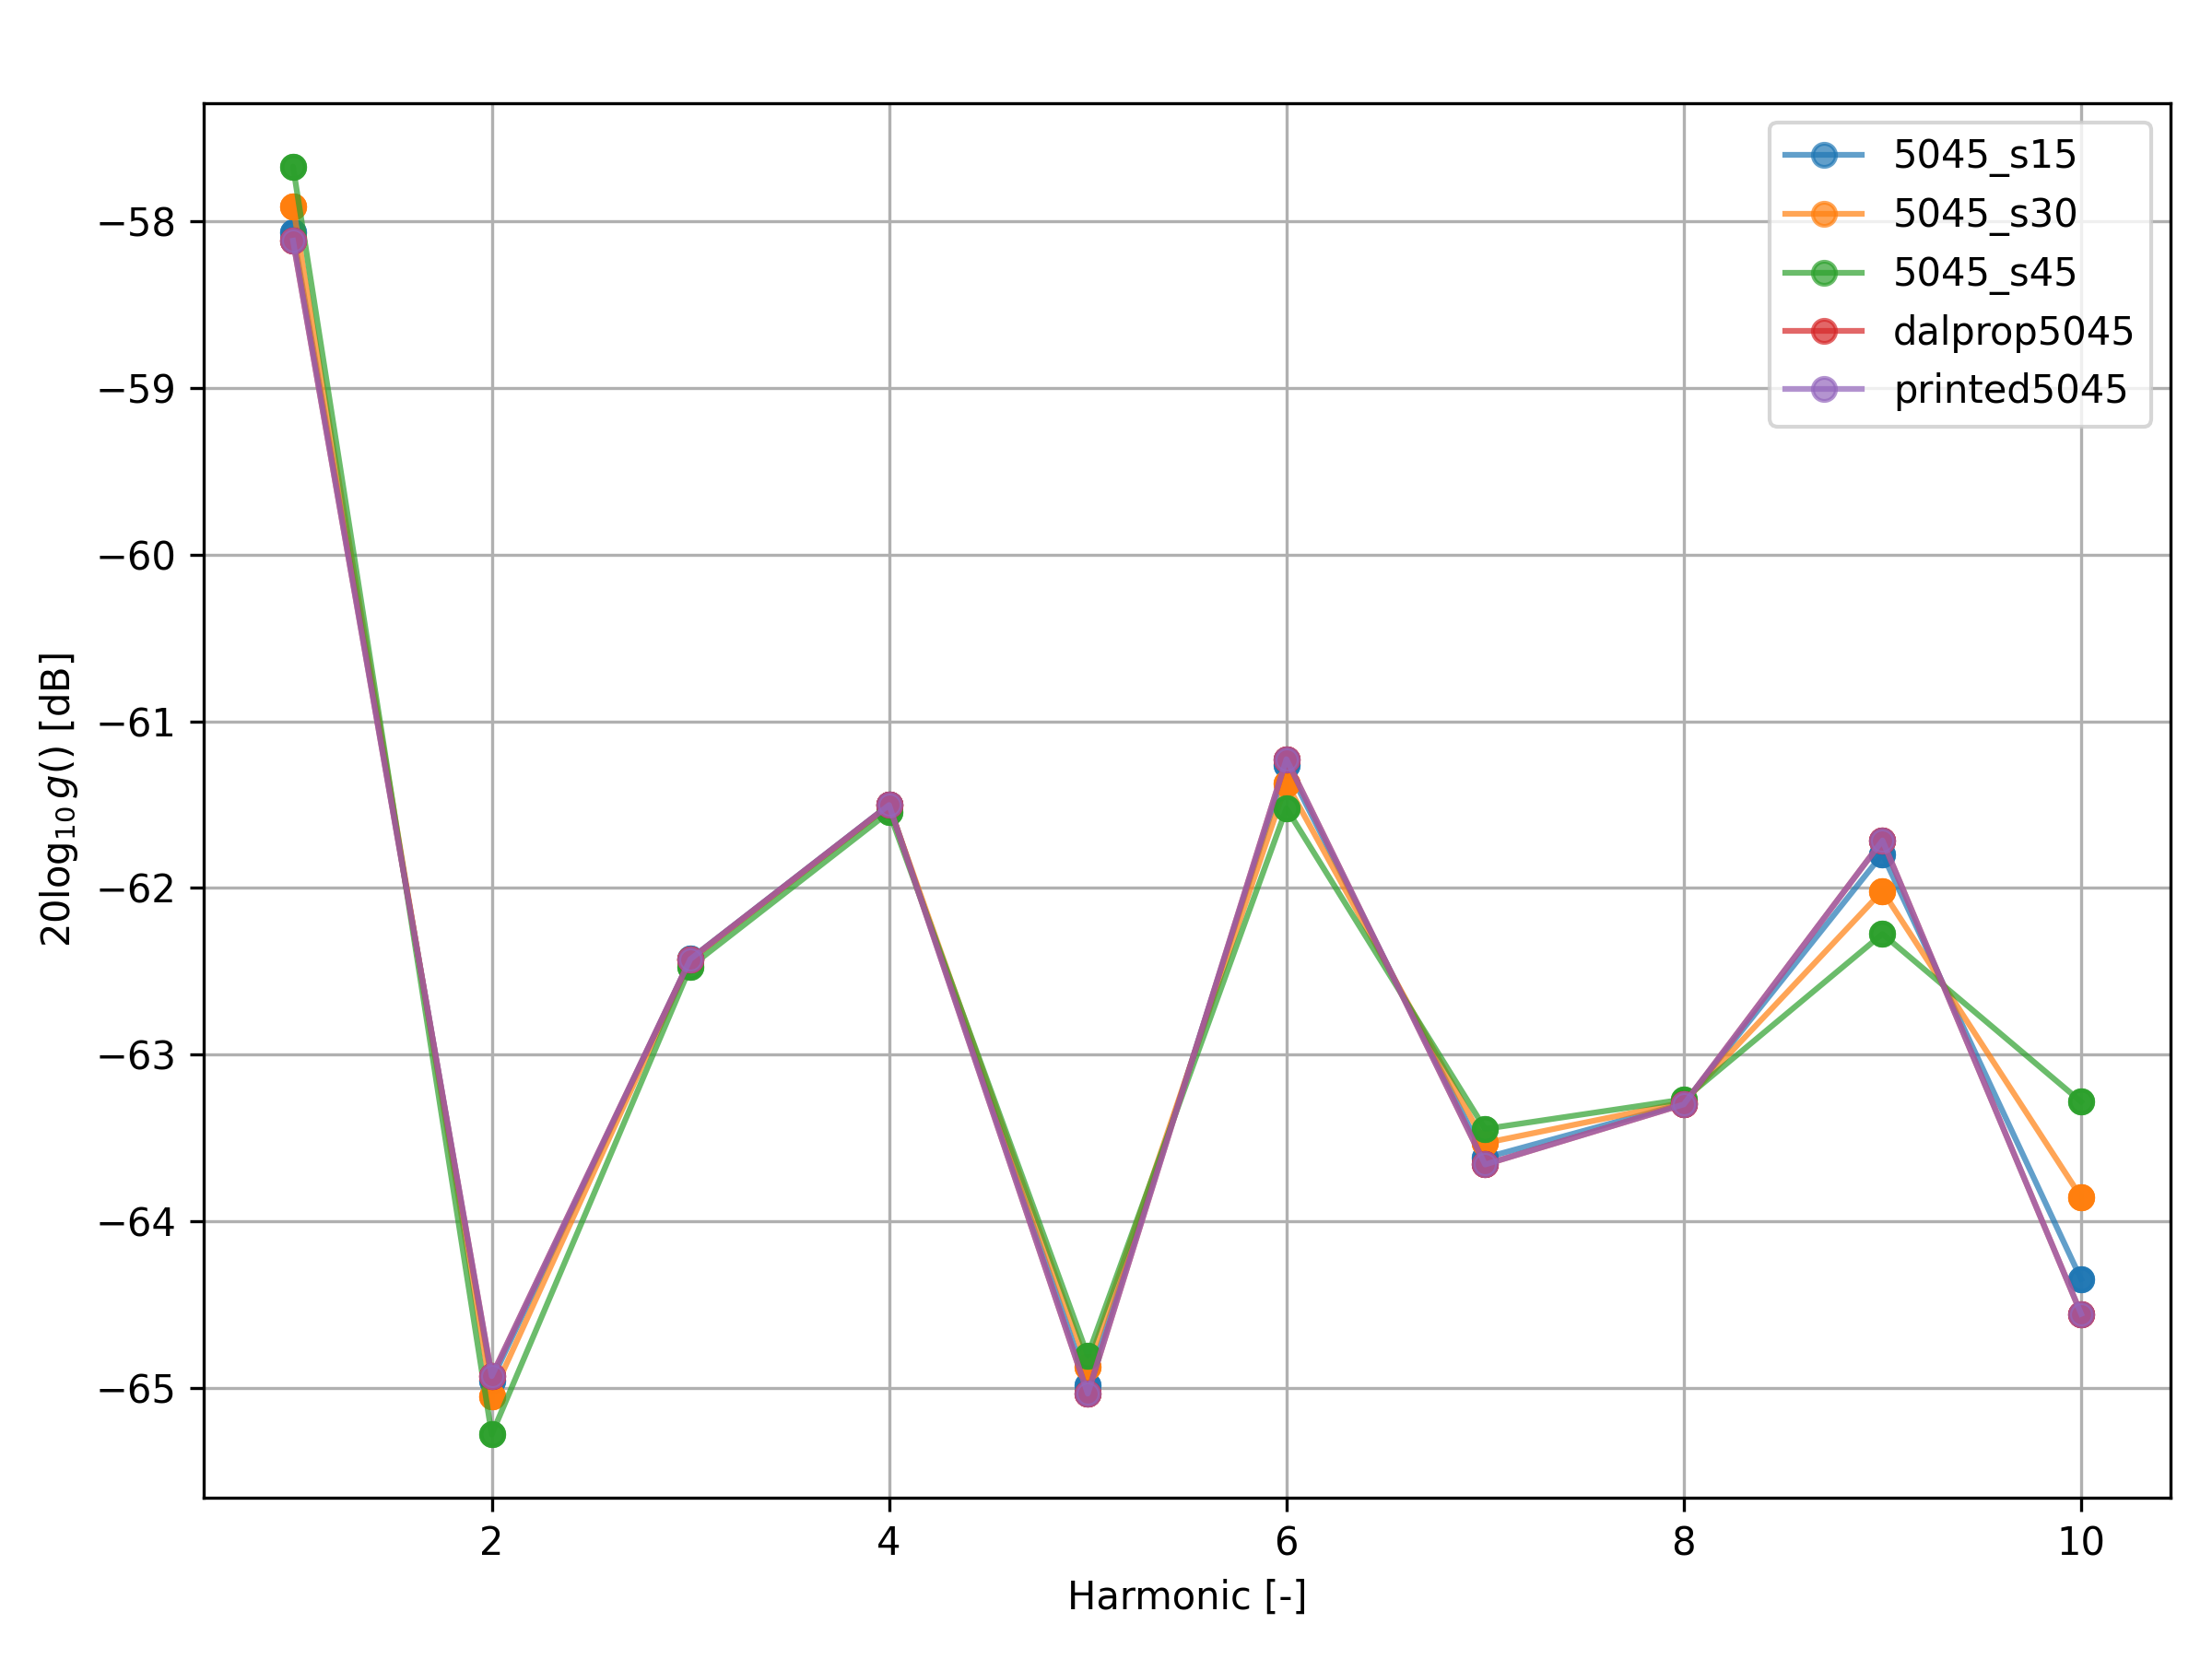
\includegraphics[width=\textwidth]{../figures/harmonic_hanson_sweep_for_135deg.pdf}
        \caption{Theoretical}
        \label{fig:harmonic_hanson_sweep_for_135deg}
    \end{subfigure}
    \begin{subfigure}[t]{0.49\textwidth}
        \centering
        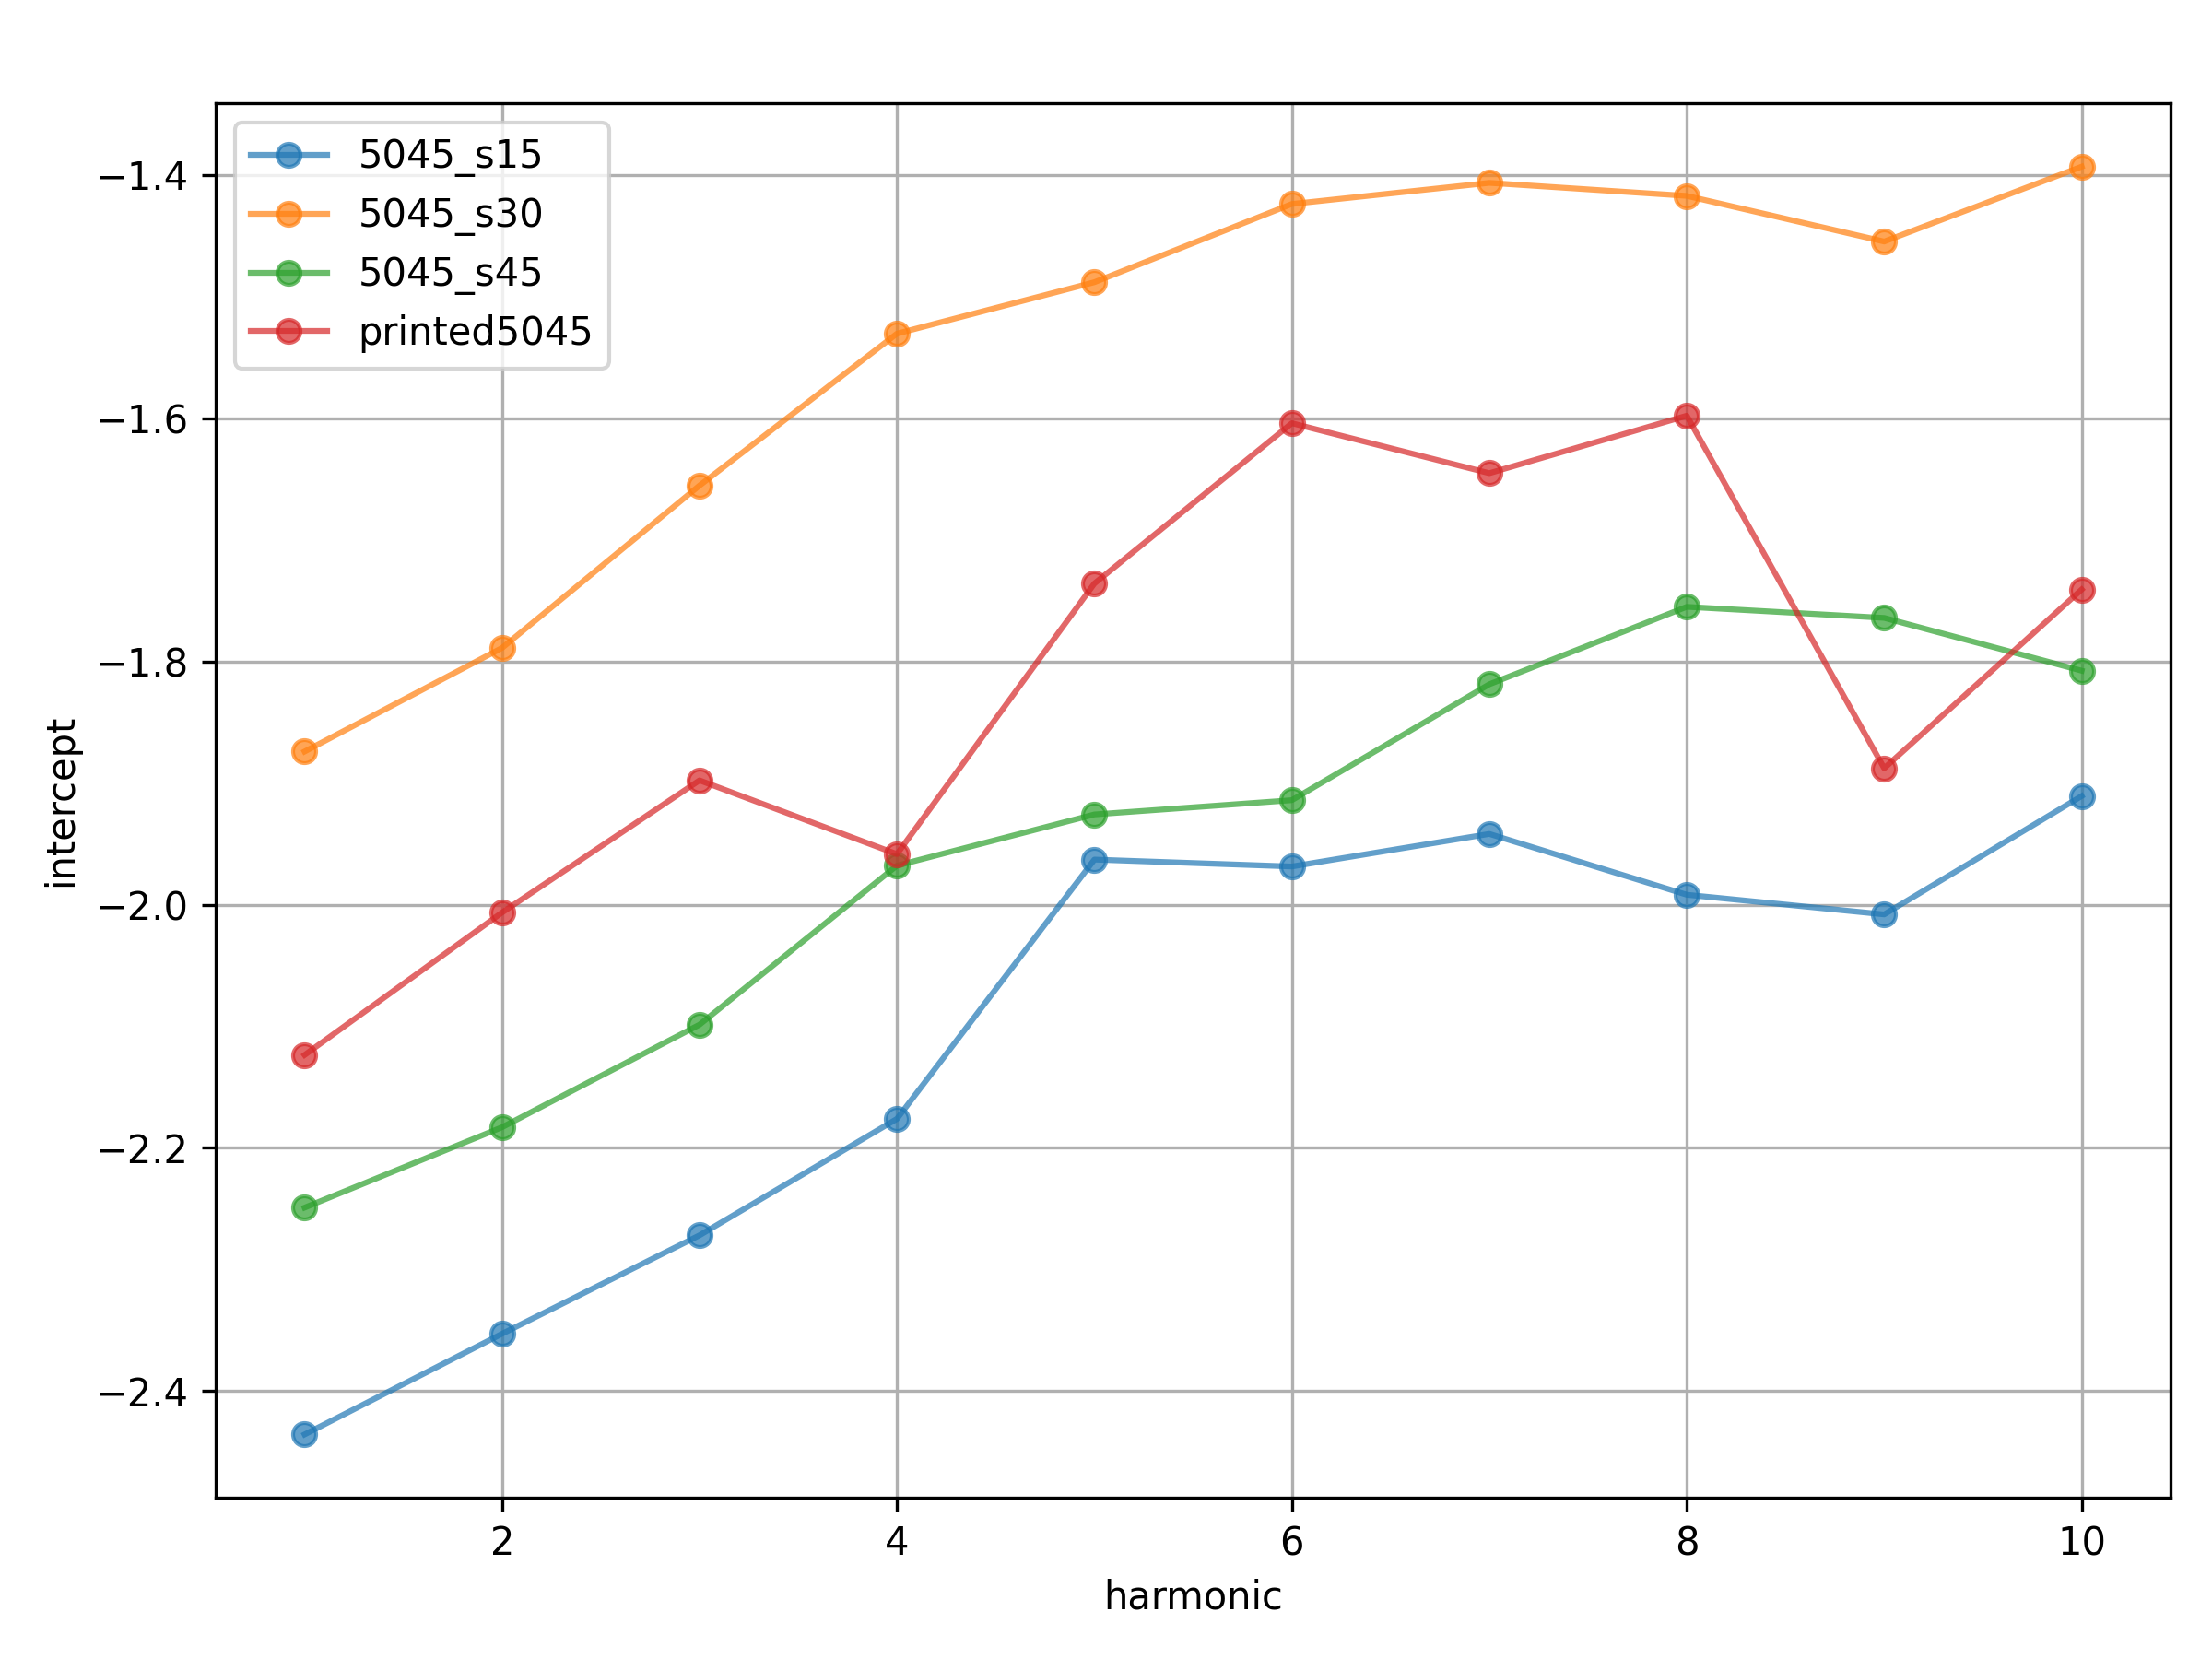
\includegraphics[width=\textwidth]{../figures/harmonic_sound_sweep_for_135deg.pdf}
        \caption{Experimental}
        \label{fig:harmonic_sound_sweep_for_135deg}
    \end{subfigure}
    \caption{Theoretical and experimental harmonic interference for differently swept propellers at $\theta = 135^\circ$.}
\end{figure}

Figures \ref{fig:harmonic_hanson_sweep_for_135deg} and \ref{fig:harmonic_sound_sweep_for_135deg} show the theoretical and experimental harmonic interference for the differently swept propellers at $\theta = 135^\circ$.
The theory shows very little difference in the harmonic interference factor $g$ for the small range of sweep angles tested.
It can also be seen that while some harmonics reduce in magnitude, other harmonics increase.
Experimental results show a significant difference in interference factor between the propellers over the range of harmonics considered.


\begin{figure}[H]
    \centering
    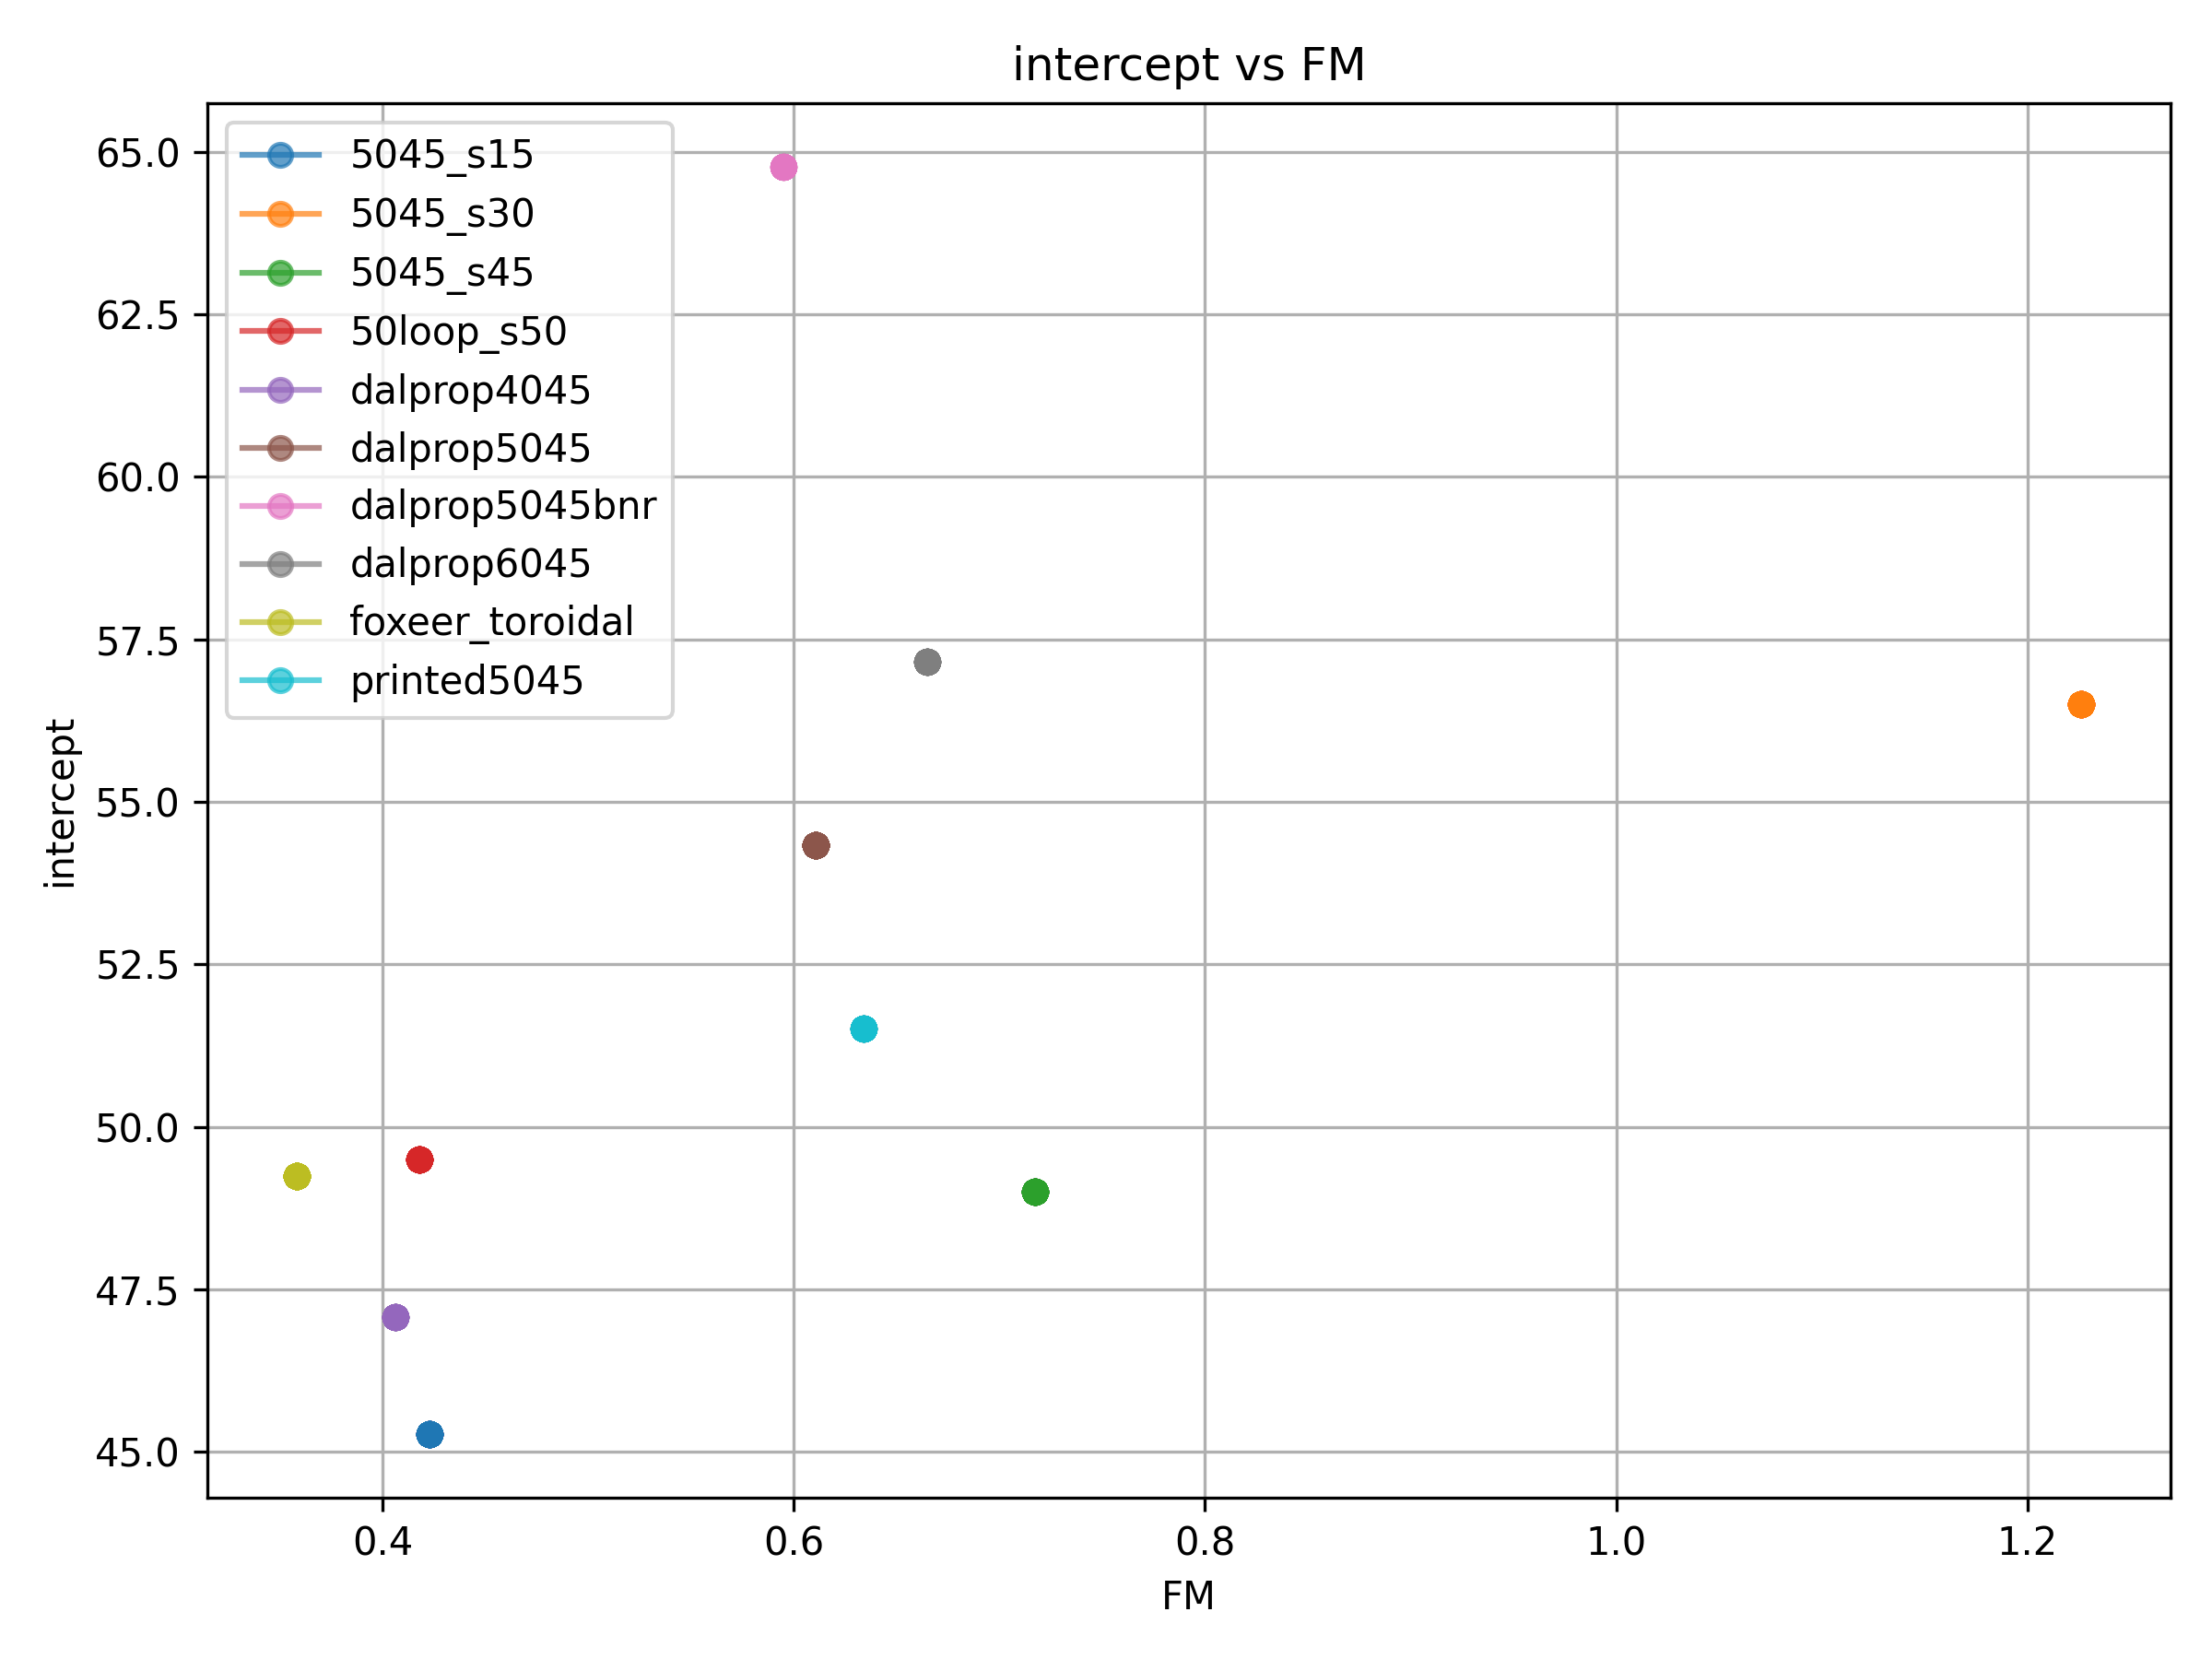
\includegraphics[width=0.8\textwidth]{../figures/prop_sound_FOM.pdf}
    \caption{First harmonic sound at $\theta = 135^\circ$ against figure of merit for all propeller designs.}
    \label{fig:prop_sound_FOM}
\end{figure}

Figure \ref{fig:prop_sound_FOM} shows the OASPL against the figure of merit for all propeller designs.

\begin{figure}[H]
    \centering
    \includegraphics[width=0.8\textwidth]{../figures/OASPLref_bar.pdf}
    \caption{}
    \label{fig:OASPLref_bar}
\end{figure}

Figure \ref{fig:OASPLref_bar} shows the OASPL for the various propellers at reference coefficients defined earlier.
High figure of merits increase the sound pressure level to the reference point, where low figure of merits reduce the sound pressure level.
This is unexpected
TODO

% load cell calibration graphs

% aerodynamic coefficient graphs

% figure of merit graphs

% microphone calibration graphs?

% spectrum of 2 and 3 blades
% identify bpf harmonics, 50hz electrical noise, motor ppf, broadband turbulence

% speed varying graphs
% distance varying graphs

% coefficient graphs?
% f graph


\section{Conclusion}

% a lot of testing was done
% software tools and experimental apparatus were developed
% results show ... ?
% agreement between theory and experiment

This report has presented key acoustic and aerodynamic performance metrics for propellers.
The definition of effective radius and speed allow for comparison of different propeller noise at reference thrust and torque coefficients.
Theory is discussed involving an interference factor which is shown to have more complex dependence than intuitively expected.
Experimental setups are carefully designed to investigate the relationships and apply comparative measures.

Which propeller was the best?

Tradeoff between noise and efficiency?

% Careful consideration of experimental was considered and 

\subsection{Improvements}

% better experimental setup
% sample longer audio recording and use welches method
% better motor vibration isolation (belt driven)
% the dynamic balancing of rotating bodies to reduce motor vibration
% massively better load cells and faster sampling rates

\begin{itemize}
    \item Sample longer audio recordings and use Welch's method to improve frequency resolution.
    \item Better isolate motor vibration, driving the propeller with a belt drive.
    \item Dynamically balance rotating bodies to reduce motor vibration.
    \item A factory calibrated 6 axis load cell such as ATI Mini43 would provide both improved accuracy and precision in the thrust and torque measurements.
        An improved data acquisition system would also allow for faster sampling rates to investigate motor cogging.
\end{itemize}

% better theoretical models
%% accounting for swirl and tip losses in current solver
%% interpolating airfoil data with reynolds number in current solver
%% panel method, wake vortex model
%% inclusion of volume displacement noise

\subsection{Future Work}
Alongside the improvements mentioned in the previous section, there are a number of avenues for future work.
The dependence of interference factor with propeller radius was not investigated and may show significant differences,
reducing the suitability of the performance metric.
% what questions were left unanswered
The comparative measure discussed can be implemented in an objective function 

% design work
% optimisation work of designs using an objective function
% integration of psychoacoustic models

\section{Appendix}

\subsection{Comparison of swirl and tiploss for BEM}

\begin{figure}[H]
    \centering
    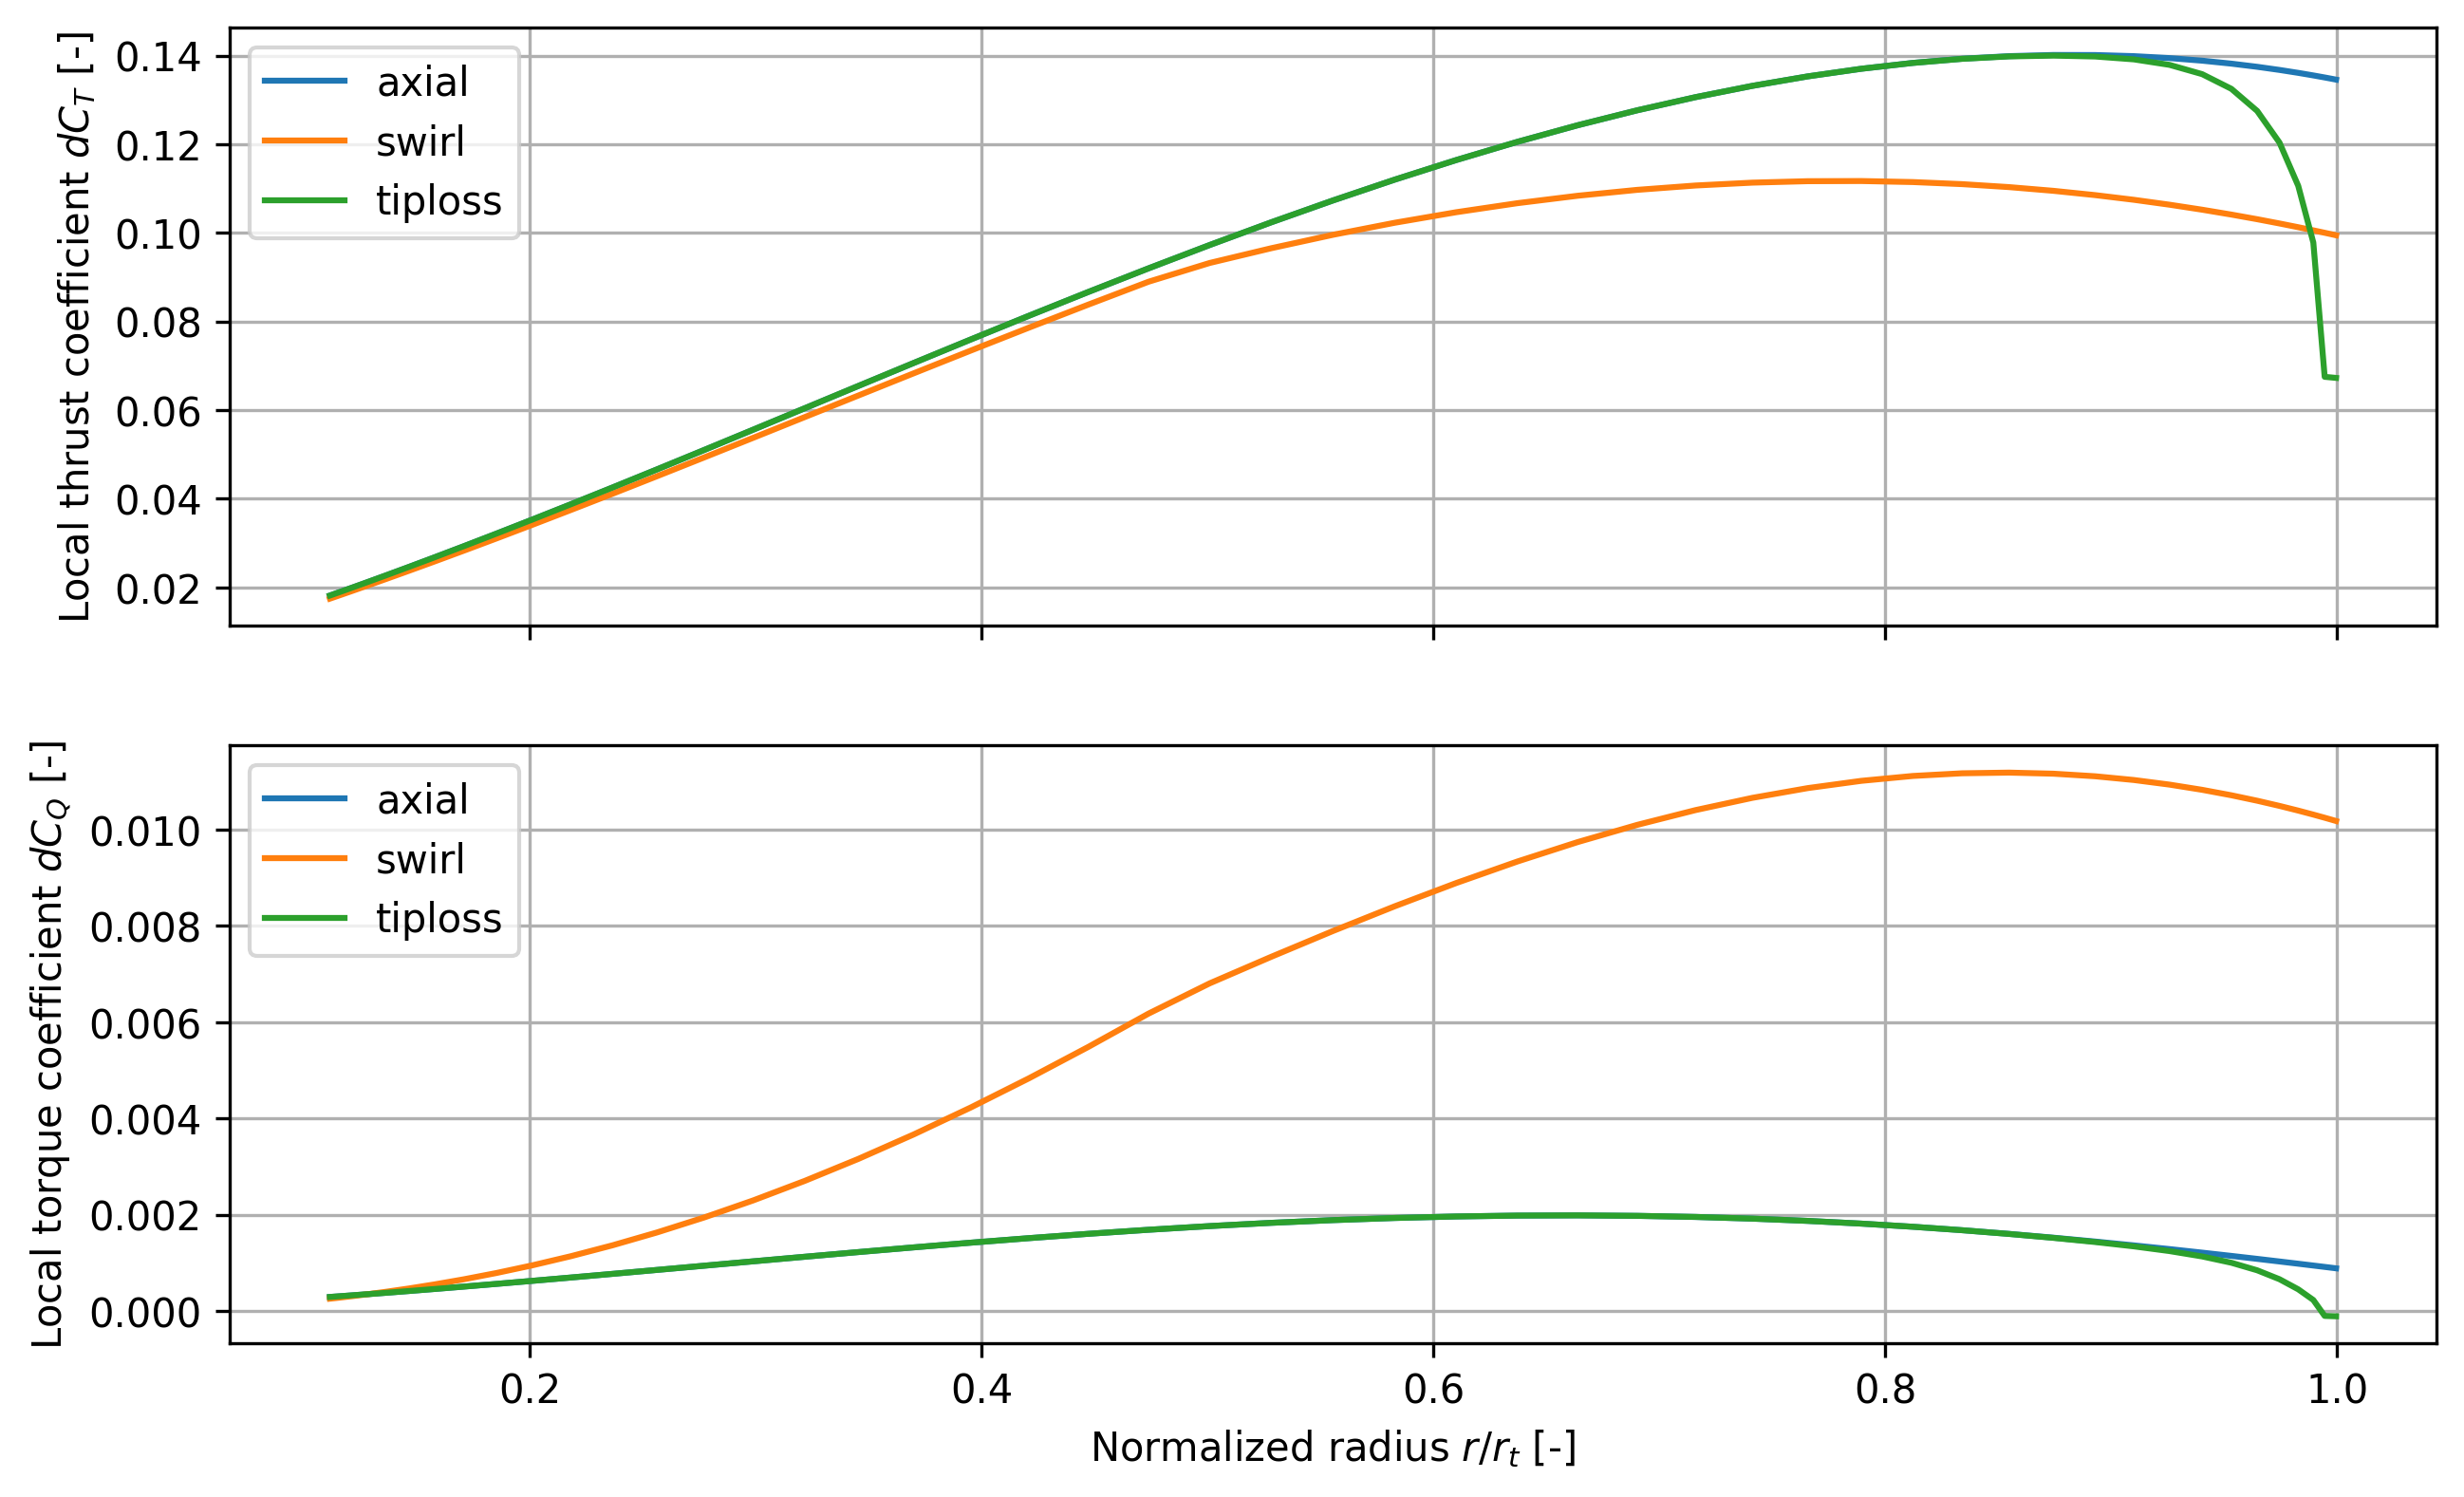
\includegraphics[width=0.8\textwidth]{../figures/bem_comparison.pdf}
    \caption{Comparison of the BEM solver with and without swirl and tip losses.}
    \label{fig:bem_comparison}
\end{figure}

\subsection{Calculation of stand resonant frequency \label{sec:appendix_stand_frequency}}

For rubber feet with a Young's modulus of $E = 10^6$, the total area of the feet is $A = 8 * \pi D^2/4$ where $D$ was measured to be 30mm.
The length of the feet $L=30mm$ and the mass of the stand was measured to be $m=5.7kg$.
The stiffness is calculated as $k = EA/L = 1.13 \times 10^6 N/m$.
The natural frequency is then $f = \frac{1}{2\pi} \sqrt{\frac{k}{m}} = 70.9 Hz$.


\subsection{Calculation of motor torque constant \label{sec:appendix_motor_calibration}}

The motor voltage constant, $k_V$, is provided by the manufacturer as 1700 KV, or 1700 revolutions per minute per unit line voltage.
The torque constant, $k_Q$, can be calculated from this using the following relationship.

\begin{equation}
    k_Q = \frac{3}{2} \frac{1}{\sqrt{3}} \frac{60}{2\pi} \frac{1}{k_V}
\end{equation}

The factors $2\pi/60$ and $1/\sqrt{3}$ simply converts this constant to radians per second per unit phase voltage.
The final $3/2$ factor arises from the conversion of 3 phase power to mechanical torque of per phase quantities.

\newpage

\subsection{Risk assessment retrospective}

The original hazard assessment included the following:
\begin{itemize}
    \item Self built low voltage, high current power source.
    \item High speed rotating propellers.
\end{itemize}
As the project progressed however, the following hazards were identified:
\begin{itemize}
    \item LiPo battery fire hazard.
    \item Mechanical failure of high speed rotating propellers.
\end{itemize}

\newpage
\printbibliography

\end{document}
